\documentclass[pdf]{beamer}\usepackage[]{graphicx}\usepackage[]{color}
%% maxwidth is the original width if it is less than linewidth
%% otherwise use linewidth (to make sure the graphics do not exceed the margin)
\makeatletter
\def\maxwidth{ %
  \ifdim\Gin@nat@width>\linewidth
    \linewidth
  \else
    \Gin@nat@width
  \fi
}
\makeatother

\definecolor{fgcolor}{rgb}{0.345, 0.345, 0.345}
\newcommand{\hlnum}[1]{\textcolor[rgb]{0.686,0.059,0.569}{#1}}%
\newcommand{\hlstr}[1]{\textcolor[rgb]{0.192,0.494,0.8}{#1}}%
\newcommand{\hlcom}[1]{\textcolor[rgb]{0.678,0.584,0.686}{\textit{#1}}}%
\newcommand{\hlopt}[1]{\textcolor[rgb]{0,0,0}{#1}}%
\newcommand{\hlstd}[1]{\textcolor[rgb]{0.345,0.345,0.345}{#1}}%
\newcommand{\hlkwa}[1]{\textcolor[rgb]{0.161,0.373,0.58}{\textbf{#1}}}%
\newcommand{\hlkwb}[1]{\textcolor[rgb]{0.69,0.353,0.396}{#1}}%
\newcommand{\hlkwc}[1]{\textcolor[rgb]{0.333,0.667,0.333}{#1}}%
\newcommand{\hlkwd}[1]{\textcolor[rgb]{0.737,0.353,0.396}{\textbf{#1}}}%
\let\hlipl\hlkwb

\usepackage{framed}
\makeatletter
\newenvironment{kframe}{%
 \def\at@end@of@kframe{}%
 \ifinner\ifhmode%
  \def\at@end@of@kframe{\end{minipage}}%
  \begin{minipage}{\columnwidth}%
 \fi\fi%
 \def\FrameCommand##1{\hskip\@totalleftmargin \hskip-\fboxsep
 \colorbox{shadecolor}{##1}\hskip-\fboxsep
     % There is no \\@totalrightmargin, so:
     \hskip-\linewidth \hskip-\@totalleftmargin \hskip\columnwidth}%
 \MakeFramed {\advance\hsize-\width
   \@totalleftmargin\z@ \linewidth\hsize
   \@setminipage}}%
 {\par\unskip\endMakeFramed%
 \at@end@of@kframe}
\makeatother

\definecolor{shadecolor}{rgb}{.97, .97, .97}
\definecolor{messagecolor}{rgb}{0, 0, 0}
\definecolor{warningcolor}{rgb}{1, 0, 1}
\definecolor{errorcolor}{rgb}{1, 0, 0}
\newenvironment{knitrout}{}{} % an empty environment to be redefined in TeX

\usepackage{alltt}
\mode<presentation>
\usetheme[compress]{Singapore} %Berkeley, Palo Alto, Singapore, Warsaw
%\usetheme[compress]{Berlin} 
%\usetheme[compress]{Madrid} 
%\usecolortheme{seagull}  %Beaver, dolphin, dove, lily, orchid, seagull, seahorse

%\usefonttheme{serif}
% font themes: default, professionalfonts, serif, structurebold, structureitalicserif, structuresmallcapsserif

\usepackage{graphicx}
\usepackage{pgf}
\usepackage{array}
\usepackage{tabularx}
\usepackage{booktabs}          %% Used in risk tables
\usepackage{multirow}          %% Used in decision tables
\usepackage{multicol}          %% Used in the toc
\usepackage[T1]{fontenc}  %to use < or > in tables

%\graphicspath{C:/Users/Chantel.Wetzel/Documents/GitHub/POP_2017}
\newcolumntype{Y}{>{\centering\arraybackslash}X}
\newcommand{\specialcell}[2][c]{\begin{tabular}[#1]{@{}c@{}}#2\end{tabular}}
\newcommand{\subscr}[1]{$_{\text{#1}}$}
\newcommand{\Fforty}{F_{\text{SPR}=40\%}}       % Needs to be done as $\Fforty$
\newcommand{\Bforty}{B_{\text{SPR}=40\%}}

\setbeamersize{text margin left=0.1in}
\setbeamersize{text margin right=0.1in}

\definecolor{pageCol}{rgb}{0.5,0.5,1.0}

\usepackage{tikz}

\usebackgroundtemplate{
  \tikz[overlay,remember picture] 
  \node[opacity=0.3, at=(current page.south east),anchor=south east,inner sep=0pt] {
    
\includegraphics[height=0.5in]{noaalogo.jpg}};
}

\setbeamertemplate{footline}
{
  \begin{beamercolorbox}[wd=.05\paperwidth,ht=0ex,dp=0ex,left]{framenumber in head/foot}%
    \insertframenumber/\inserttotalframenumber
    
  \end{beamercolorbox}%
}
\setbeamercolor{footline}{fg=pageCol}

\newcounter{saveenumi}

%<<load_everything, echo = FALSE, message=FALSE, results='hide', warning=FALSE>>=
%     source("C:/Users/Chantel.Wetzel/Documents/GitHub/POP_2017/Presentation/0_Run_Model_Presentation.R")
%      #create.plots = TRUE
%      #Run.Model.Present(create.plots)
%     source("C:/Users/Chantel.Wetzel/Documents/GitHub/POP_2017/Presentation/tables/catch.R")
%@

%<<load_mod1, echo = FALSE, message=FALSE, results='hide', warning=FALSE>>=
%  load("C:/Users/Chantel.Wetzel/Documents/GitHub/POP_2017/Presentation/SS_output.RData")
%@

\newcommand{\mytableofcontents}{
  \begin{frame}[t]
  \frametitle{Outline}
  %\begin{multicols}{2}
  \tableofcontents[
    currentsection, sectionstyle=show/show, subsectionstyle=show/show/hide,
  ]
  %\end{multicols}
  \end{frame}
}
\AtBeginSection[]{\mytableofcontents}

%------------------------------------------------------------------------------------
% Title Page
%------------------------------------------------------------------------------------
\title{Pacific ocean perch 2017 Assessment}
\subtitle{Biology and Data}
\author{Chantel Wetzel$^{1}$\\
        Lee Cronin-Fine$^{2}$}
\institute[NWFSC]{
Northwest Fisheries Science Center$^1$ \\
University of Washington$^2$ \\
\medskip
}
\date{{\footnotesize STAR Panel \\ June 26-30, 2017}}
\IfFileExists{upquote.sty}{\usepackage{upquote}}{}
\begin{document}

\begin{frame}
  \titlepage
\end{frame}


%------------------------------------------------------------------------------------
\section{Model Summary}
%------------------------------------------------------------------------------------
\subsection{Landings}
\begin{frame}{Landings}
  \begin{center}
    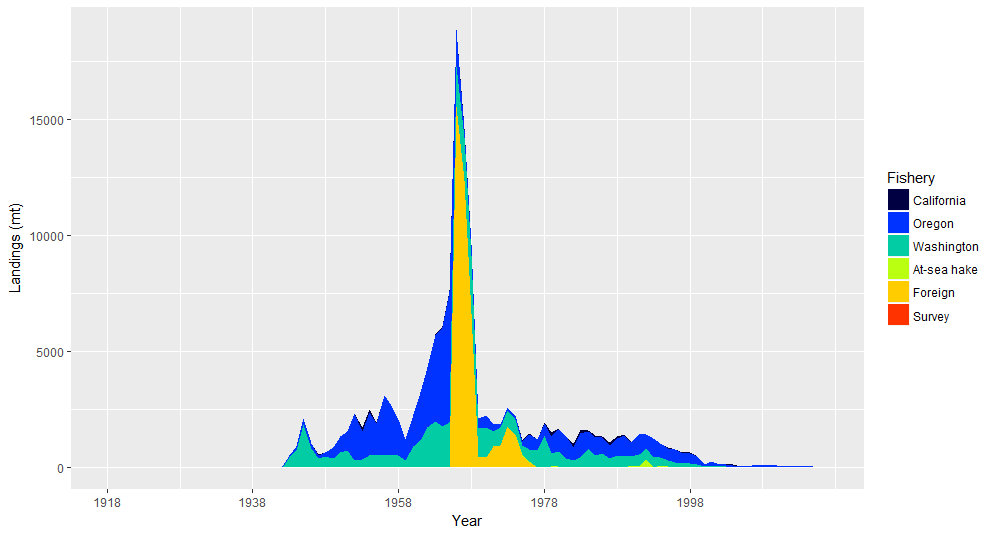
\includegraphics[scale = 0.40]{figures/catches.png}
  \end{center}
\end{frame}

\begin{frame}{Landings without the Foreign Catches}
  \begin{center}
    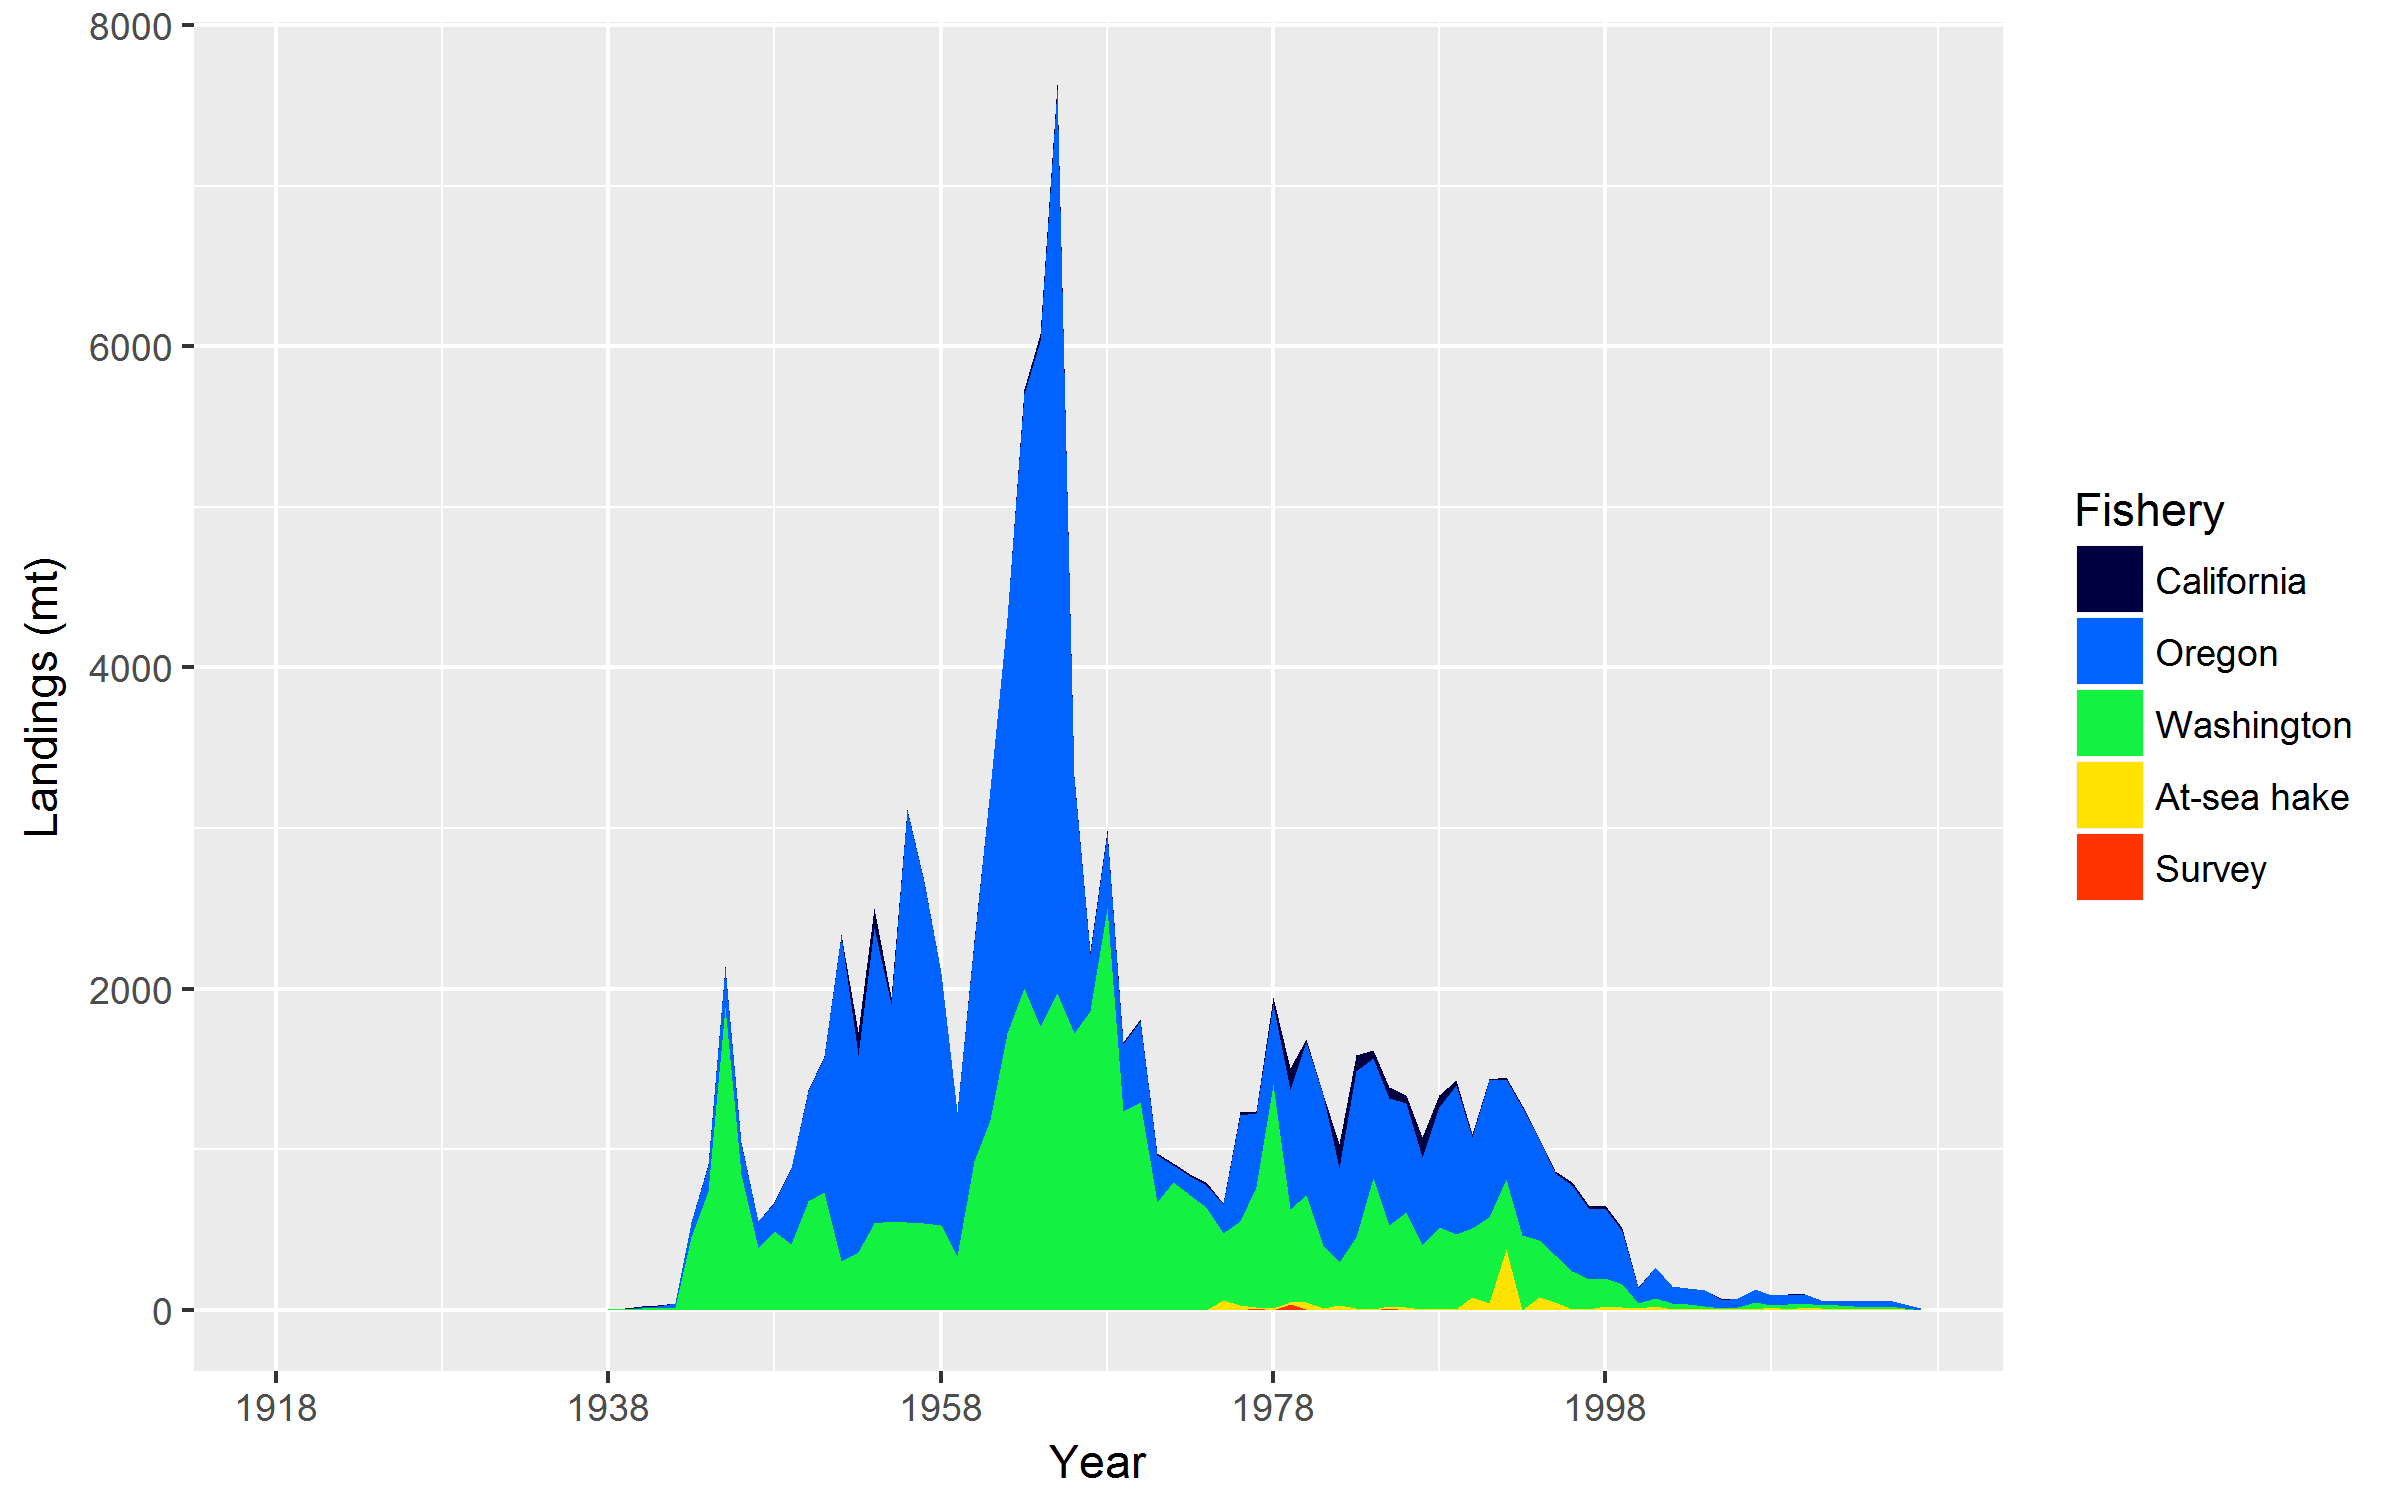
\includegraphics[scale = 0.40]{figures/POP_Landings_wo_Foreign.png}
  \end{center}
\end{frame}

\begin{frame}{Landings over the Last 10-years}
  \begin{table}[ht]
  \centering
  \begin{tabular}{p{0.4in}p{0.4in}p{0.4in}p{0.4in}p{0.4in}p{0.4in}p{0.6in}}
  Year & CA & OR & WA & At-sea hake & Survey & Total Landings \\ 
  \hline
  2007 & 0.15 & 83.65 & 45.12 & 4.05 & 0.58 & 133.55 \\ 
  2008 & 0.39 & 58.64 & 16.61 & 15.93 & 0.80 & 92.36 \\ 
  2009 & 0.92 & 58.74 & 33.22 & 1.56 & 2.72 & 97.17 \\ 
  2010 & 0.14 & 58.00 & 22.29 & 16.87 & 1.68 & 98.98 \\ 
  2011 & 0.12 & 30.26 & 19.66 & 9.17 & 1.94 & 61.14 \\ 
  2012 & 0.18 & 30.41 & 21.79 & 4.52 & 1.62 & 58.51 \\ 
  2013 & 0.08 & 34.86 & 14.83 & 5.41 & 1.71 & 56.89 \\ 
  2014 & 0.18 & 33.91 & 15.82 & 3.92 & 0.57 & 54.40 \\ 
  2015 & 0.12 & 38.05 & 11.41 & 8.71 & 1.59 & 59.88 \\ 
  2016 & 0.23 & 40.81 & 13.12 & 10.30 & 3.10 & 67.56 \\ 
  \hline
  \end{tabular}
  \end{table}
  Approximately 70\% of the landings are from Oregon.\\
  Vast majority of landings are from bottom-trawl gear.
\end{frame}


\subsection{Estimated Stock Size and Status}
\begin{frame}{Spawning Output}
  \begin{center}
    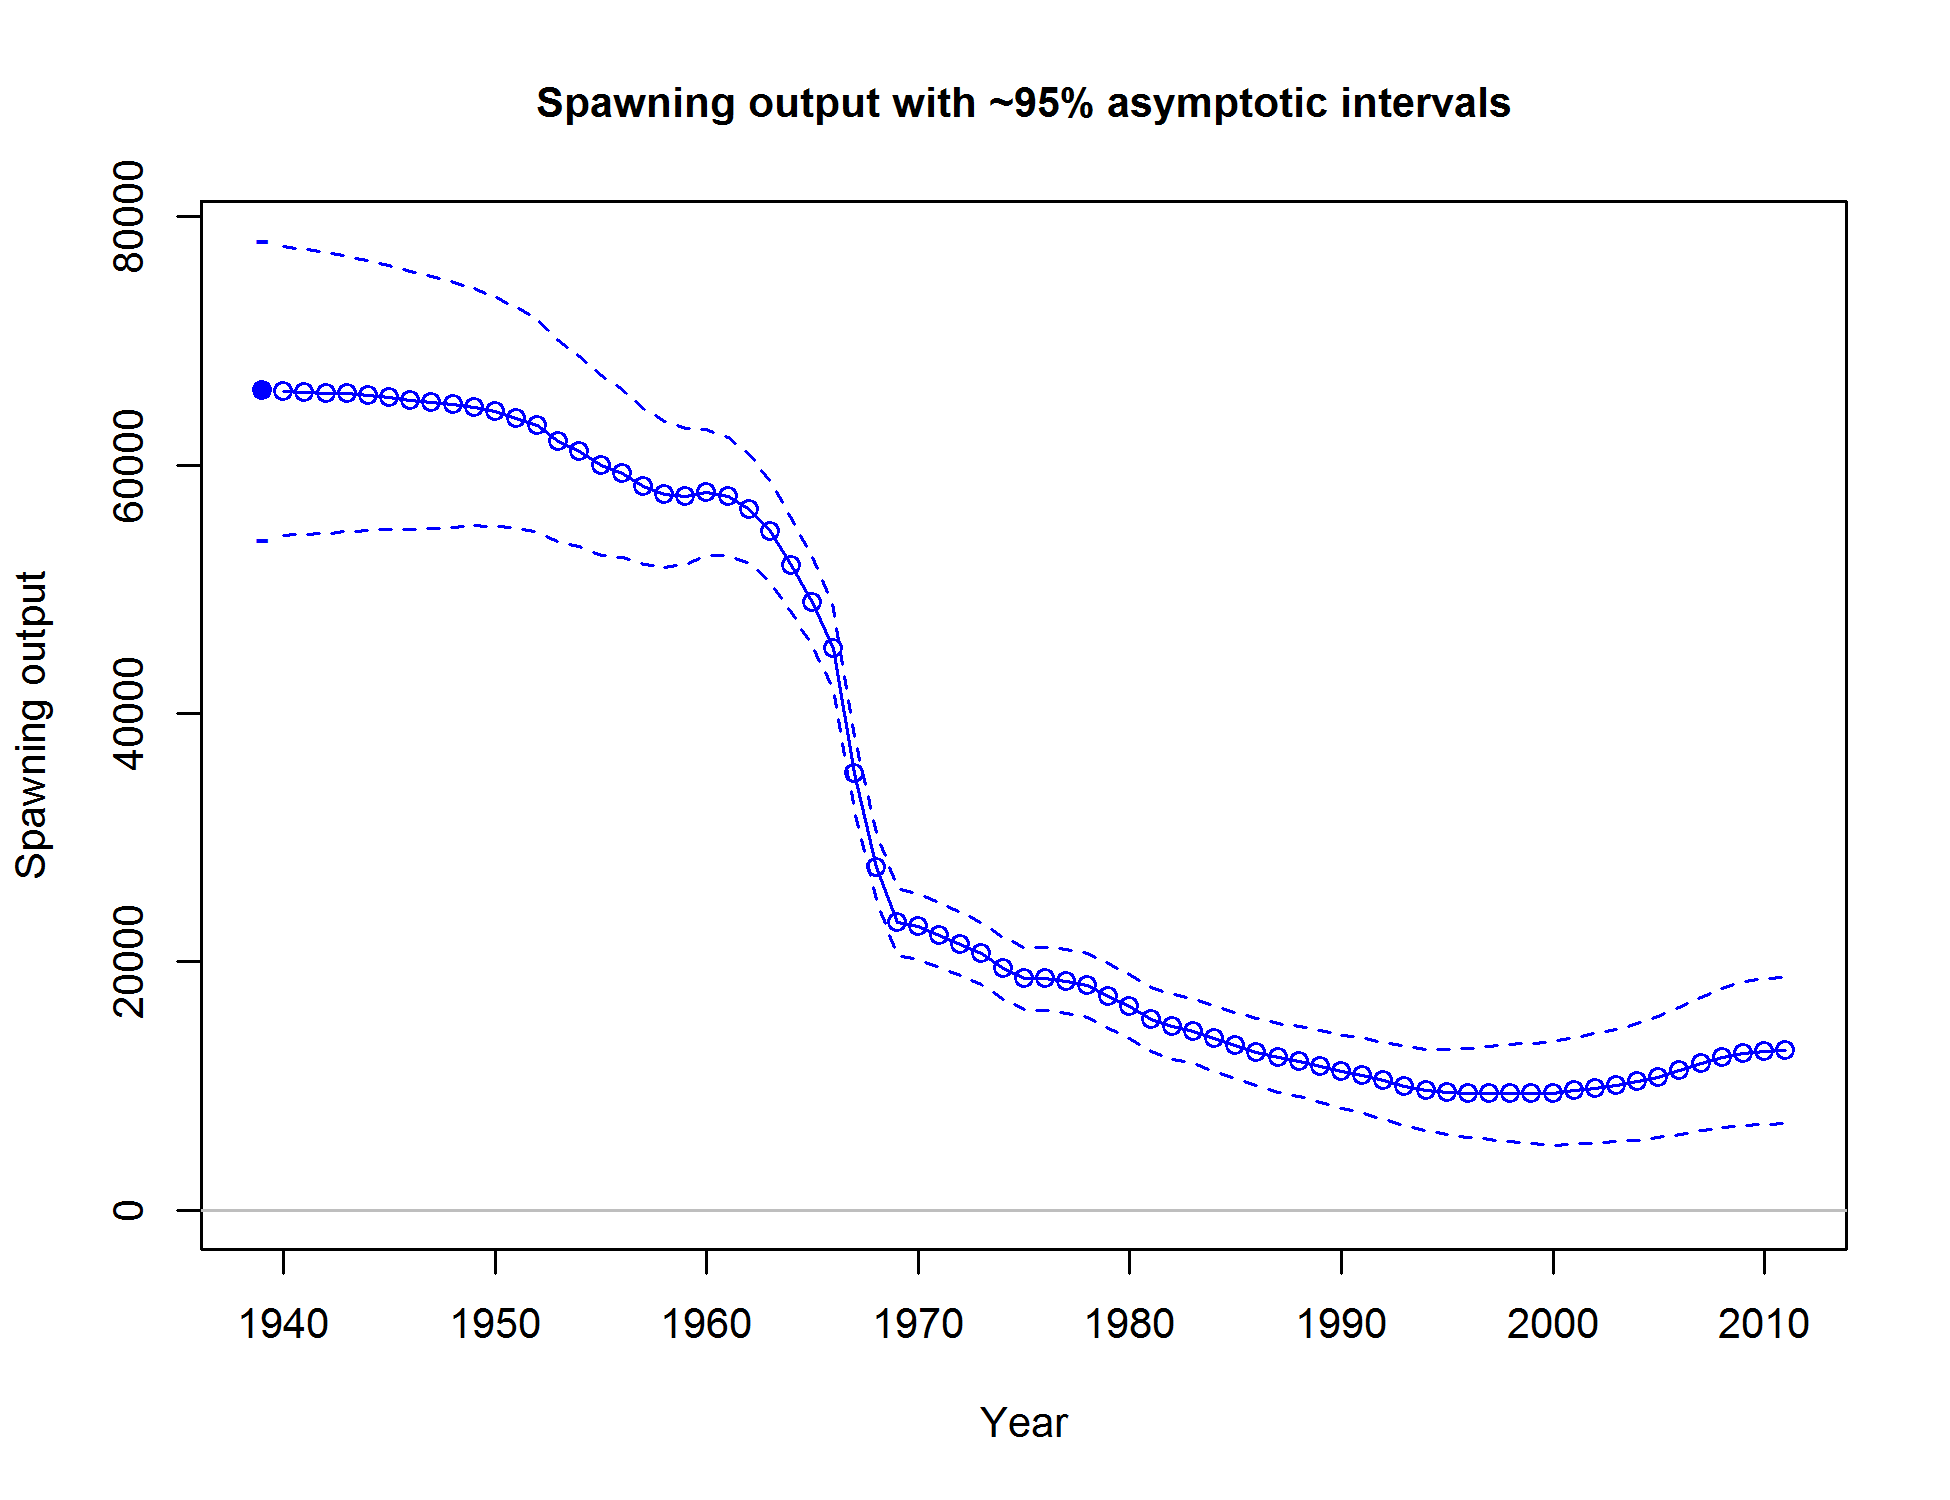
\includegraphics[scale = 0.50, trim={0cm 0cm 0cm 1.7cm}, clip]{r4ss/ts7_Spawning_output_with_95_asymptotic_intervals_intervals.png}
  \end{center}
\end{frame}


\begin{frame}{Relative Depletion}
  \begin{center}
    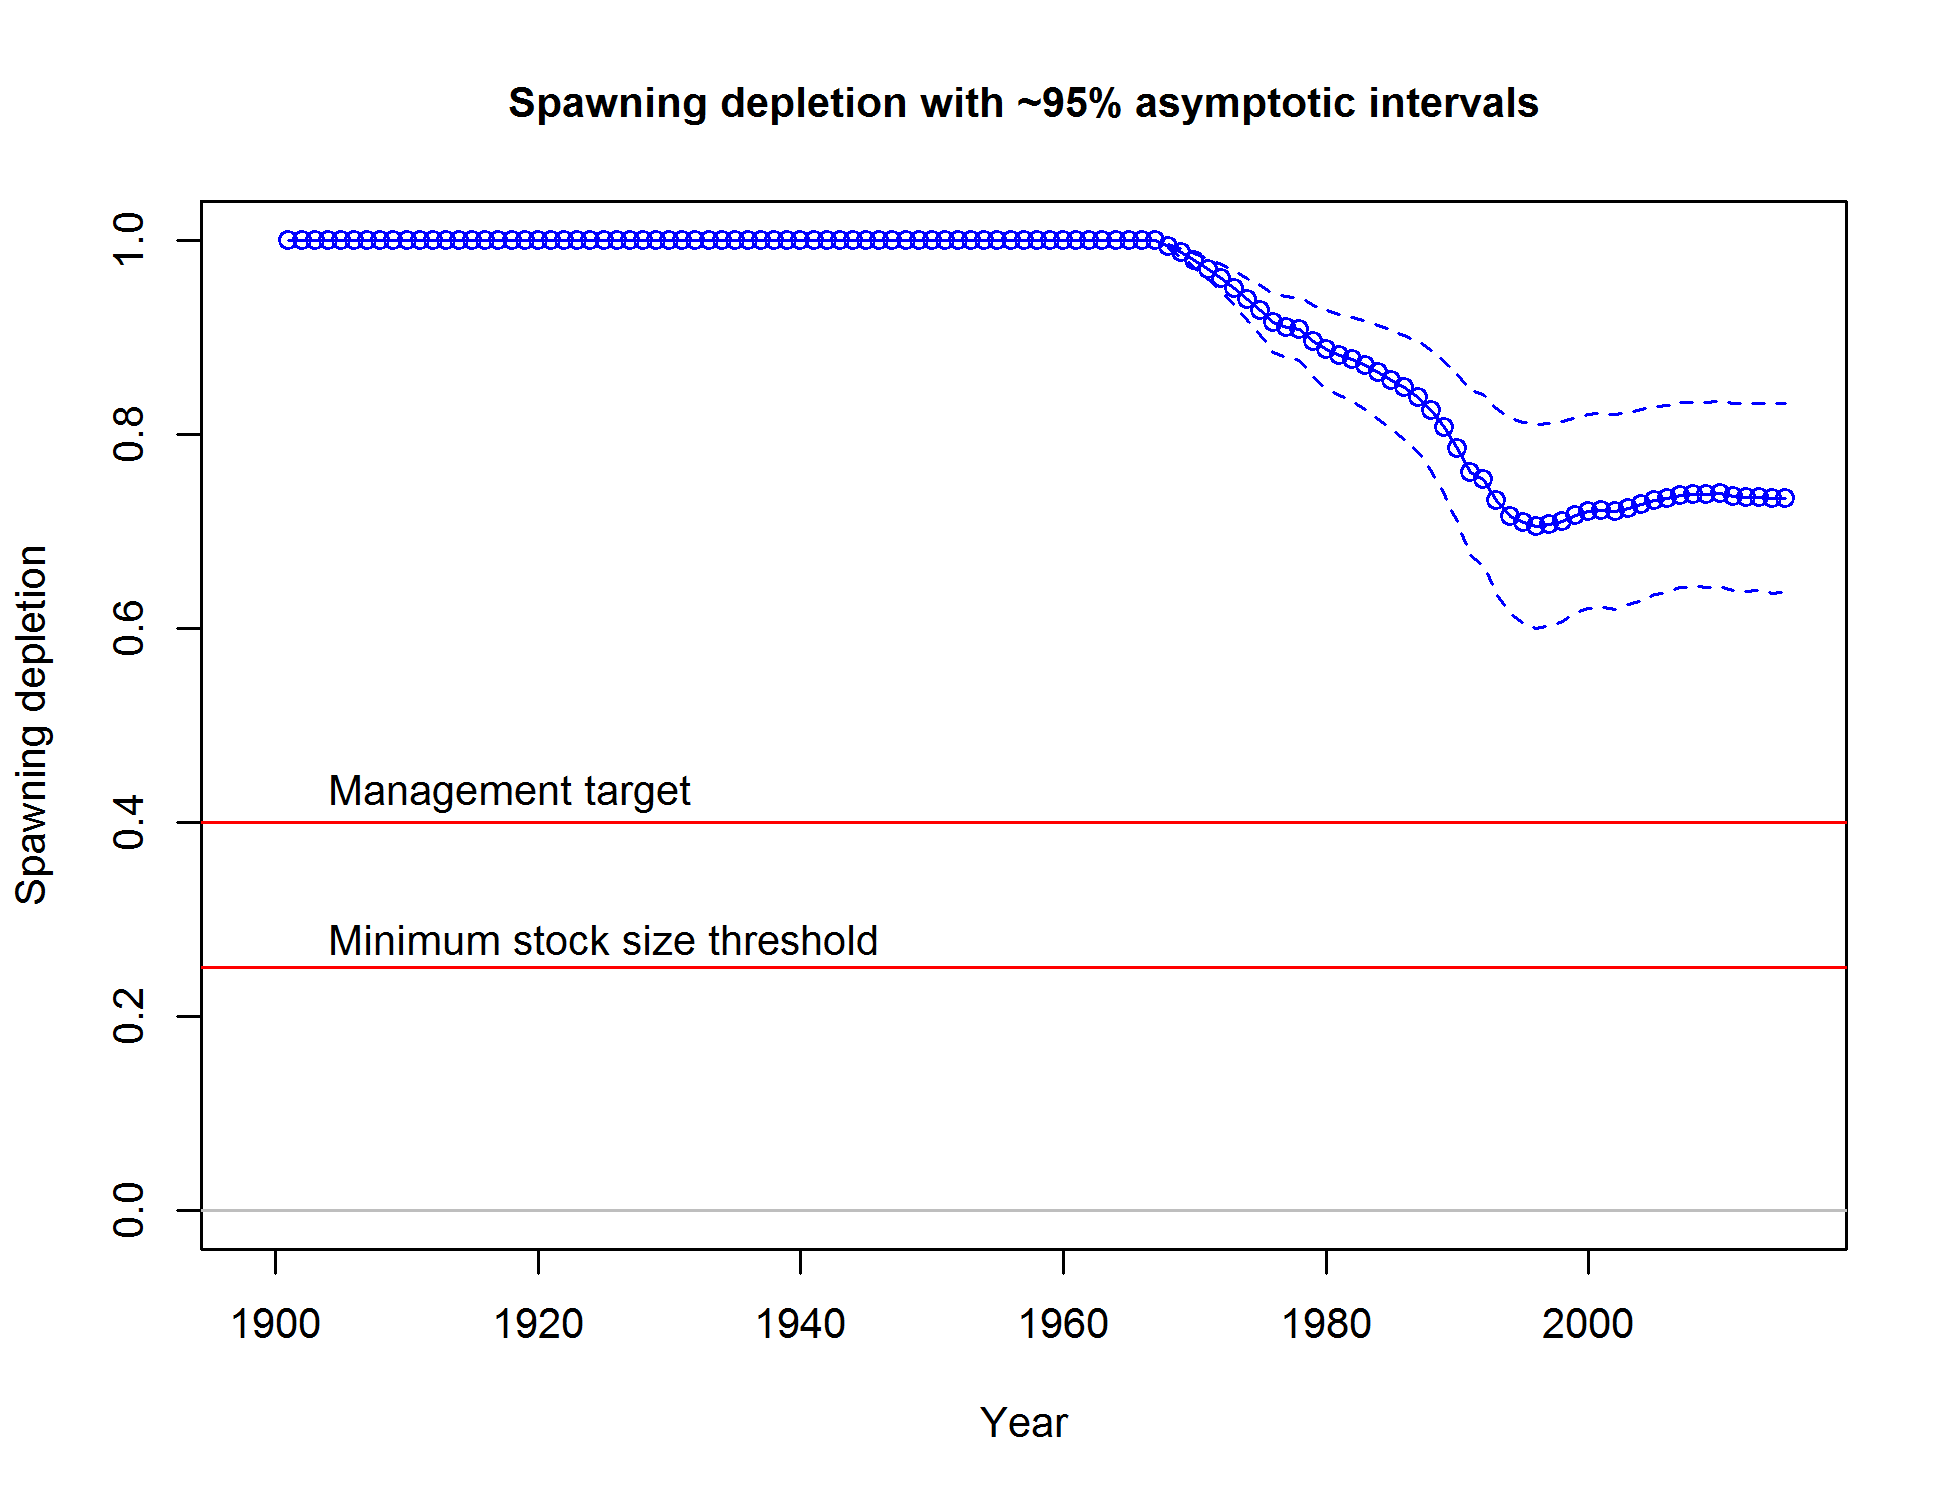
\includegraphics[scale = 0.50, trim={0cm 0cm 0cm 1.7cm}, clip]{r4ss/ts9_Spawning_depletion_with_95_asymptotic_intervals_intervals.png}
  \end{center}
  \begin{tikzpicture}[remember picture, overlay, shift = {(current page.center)}]
    \node[black] at (2.75, 1) { 74.9\%};
  \end{tikzpicture}
  %<<depletion, echo = FALSE, message=FALSE, warning=FALSE>>=
  %  depletion.print()
  %@
\end{frame}


\begin{frame}{Estimated Annual Recruitment}
  \begin{center}
    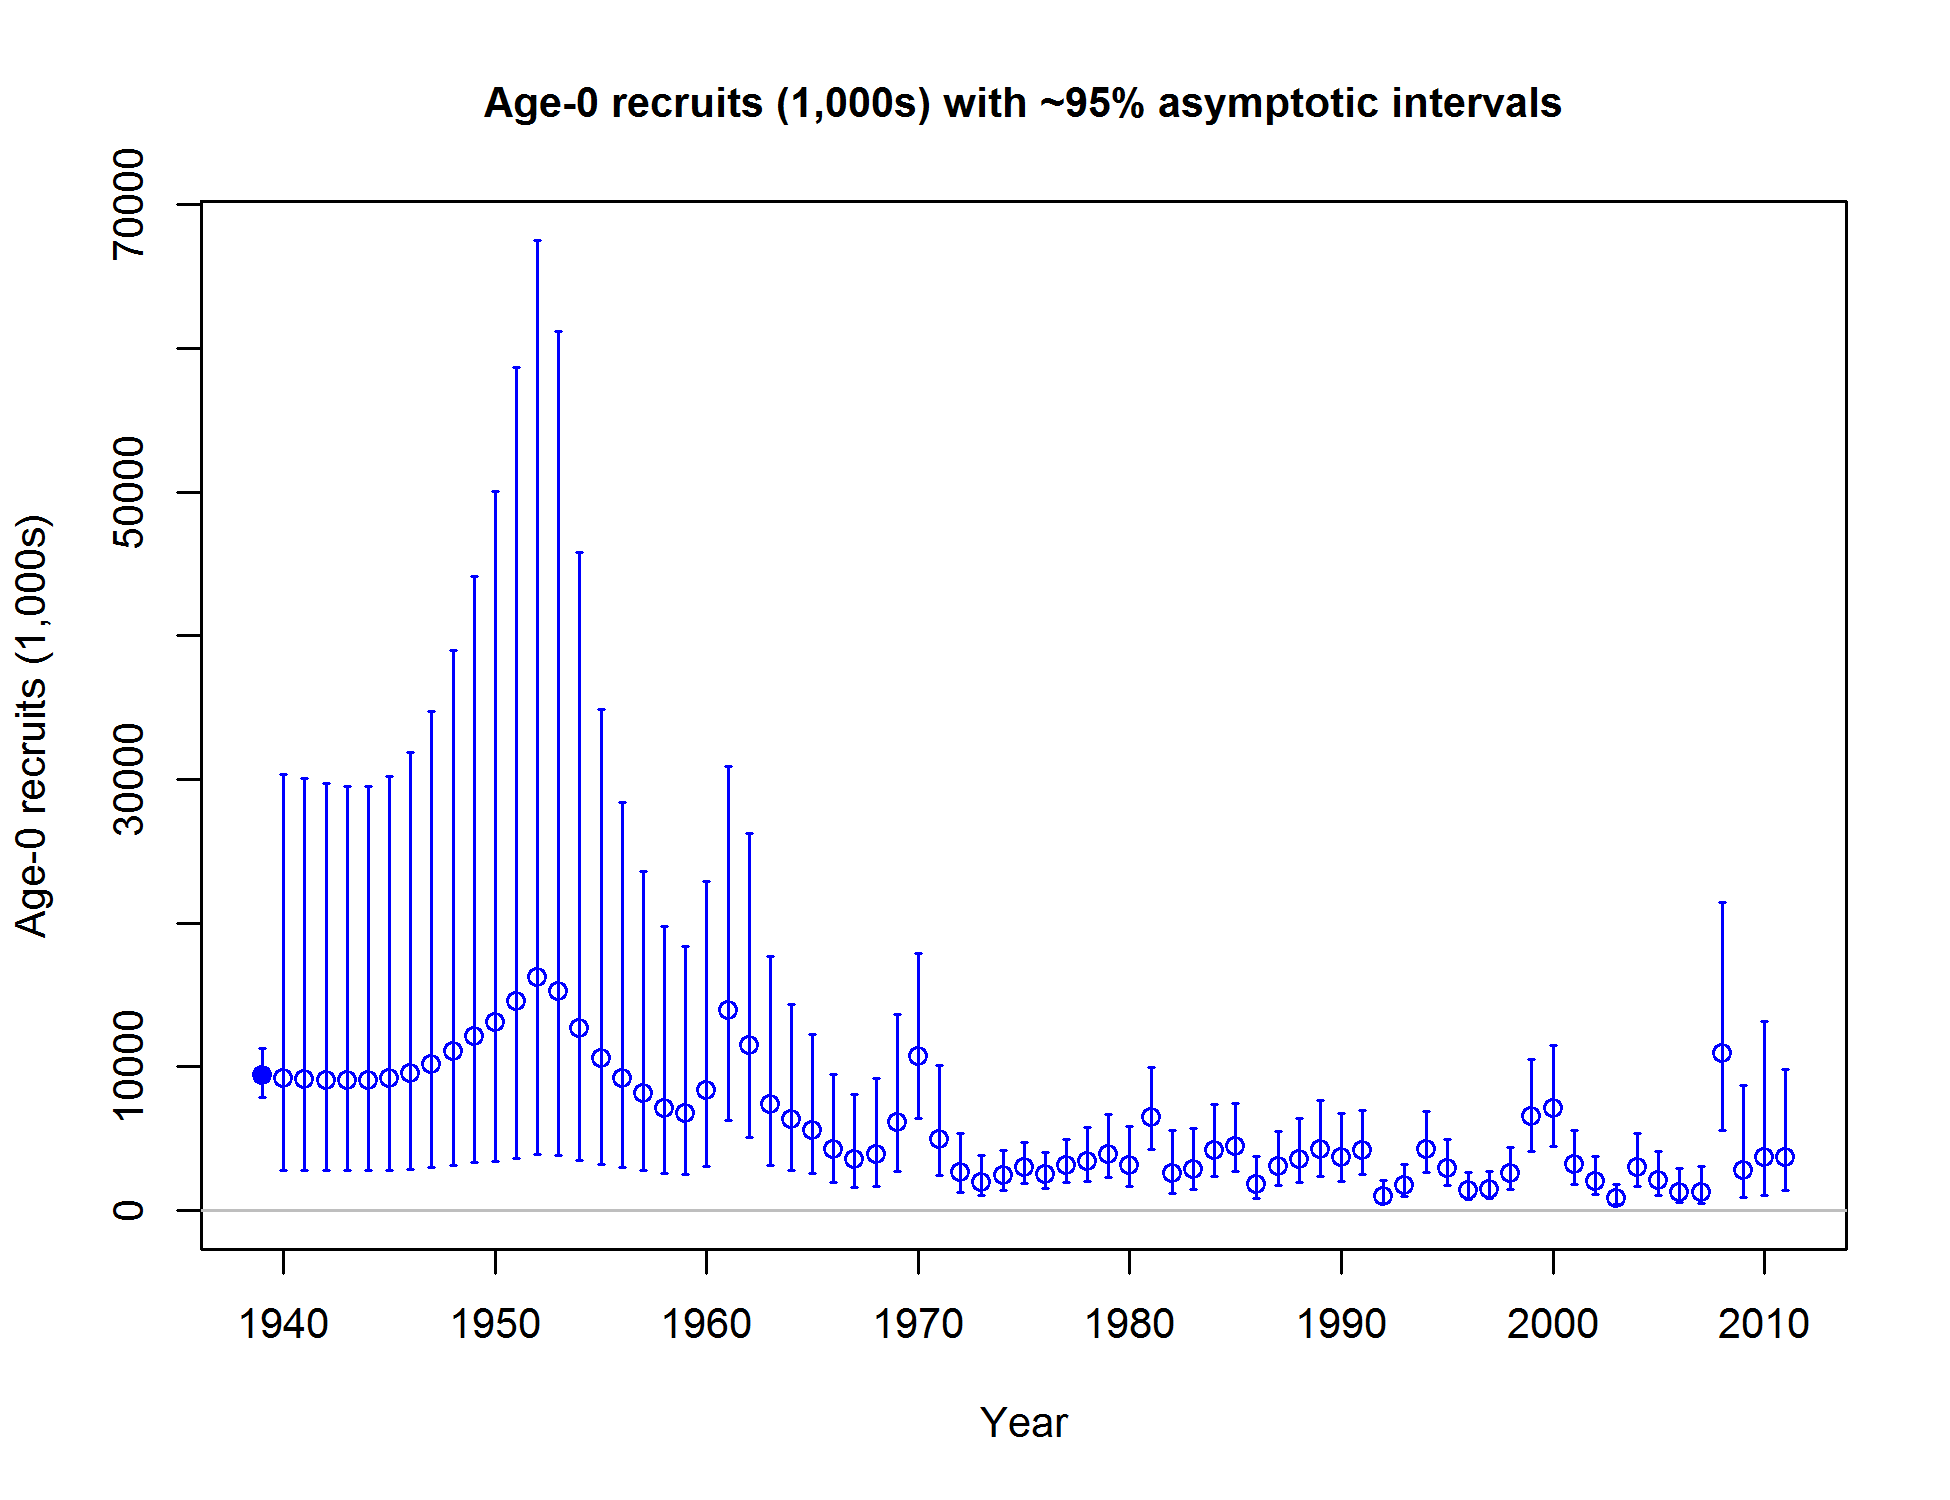
\includegraphics[scale = 0.50, trim={0cm 0cm 0cm 1.7cm}, clip]{r4ss/ts11_Age-0_recruits_(1000s)_with_95_asymptotic_intervals.png}
  \end{center}
  \begin{tikzpicture}[remember picture, overlay, shift = {(current page.center)}]
    \node[black] at (2.5, 0.75) {\tiny 2008};
    \node[black] at (3.25, -0.25) {\tiny 2013};
    \node[black] at (2.2, -0.75) {\tiny 1999 \& 2000};
  \end{tikzpicture}
\end{frame}

\begin{frame}{Estimated Annual Recruitment Deviations}
  \begin{center}
    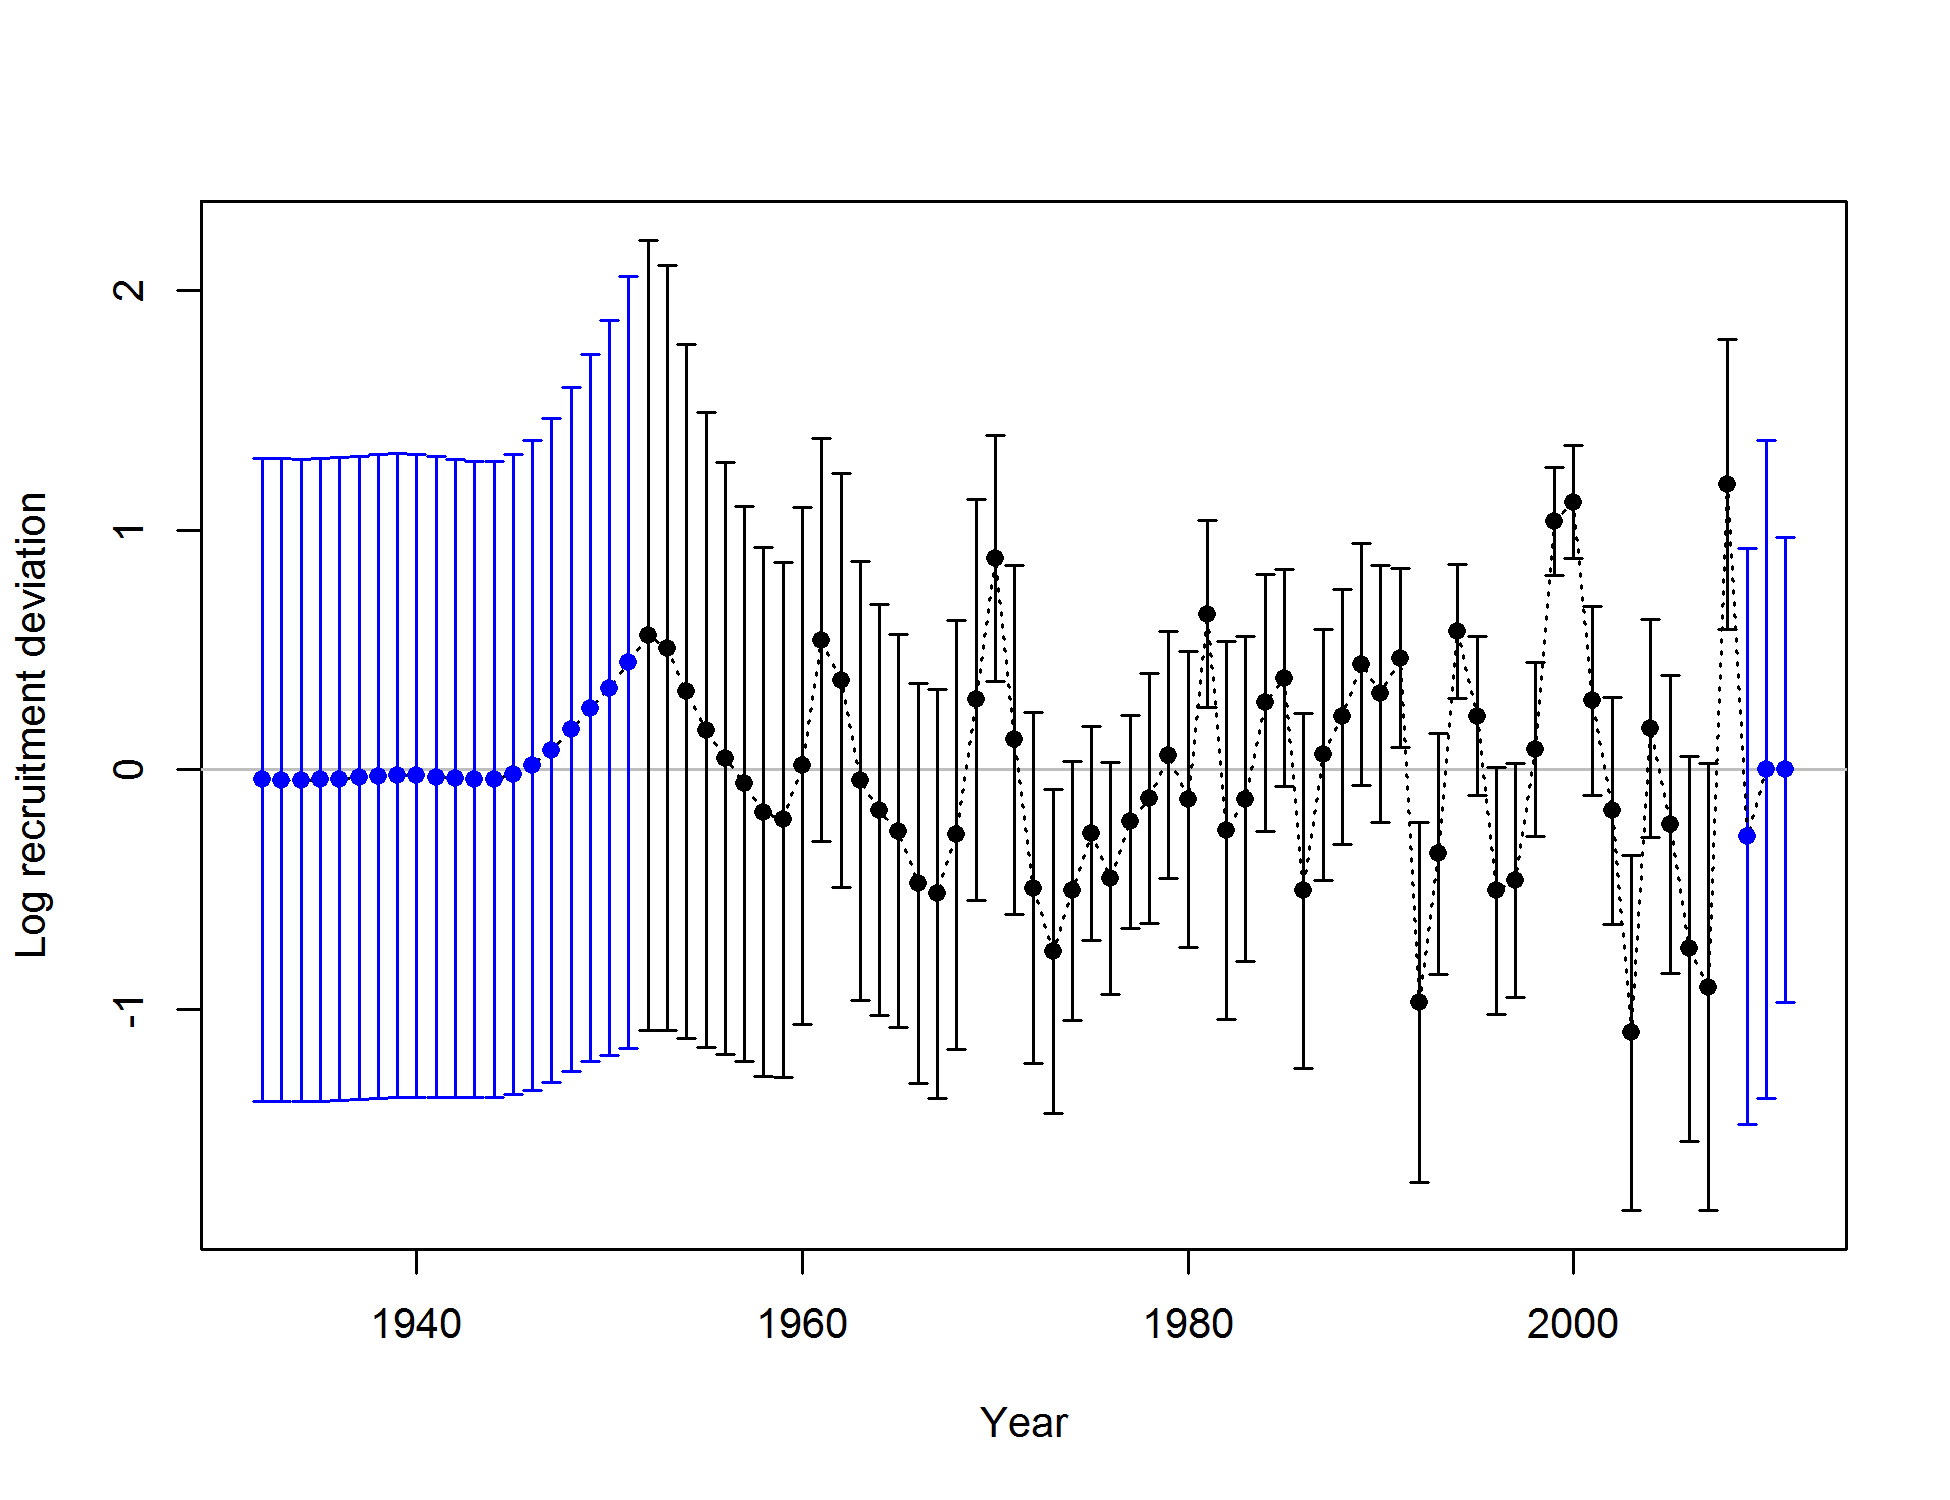
\includegraphics[scale = 0.50, trim={0cm 0cm 0cm 1.7cm}, clip]{r4ss/recdevs2_withbars.png}
  \end{center}
\end{frame}

\begin{frame}{Comparison between 2011 and 2017}
  \begin{center}
    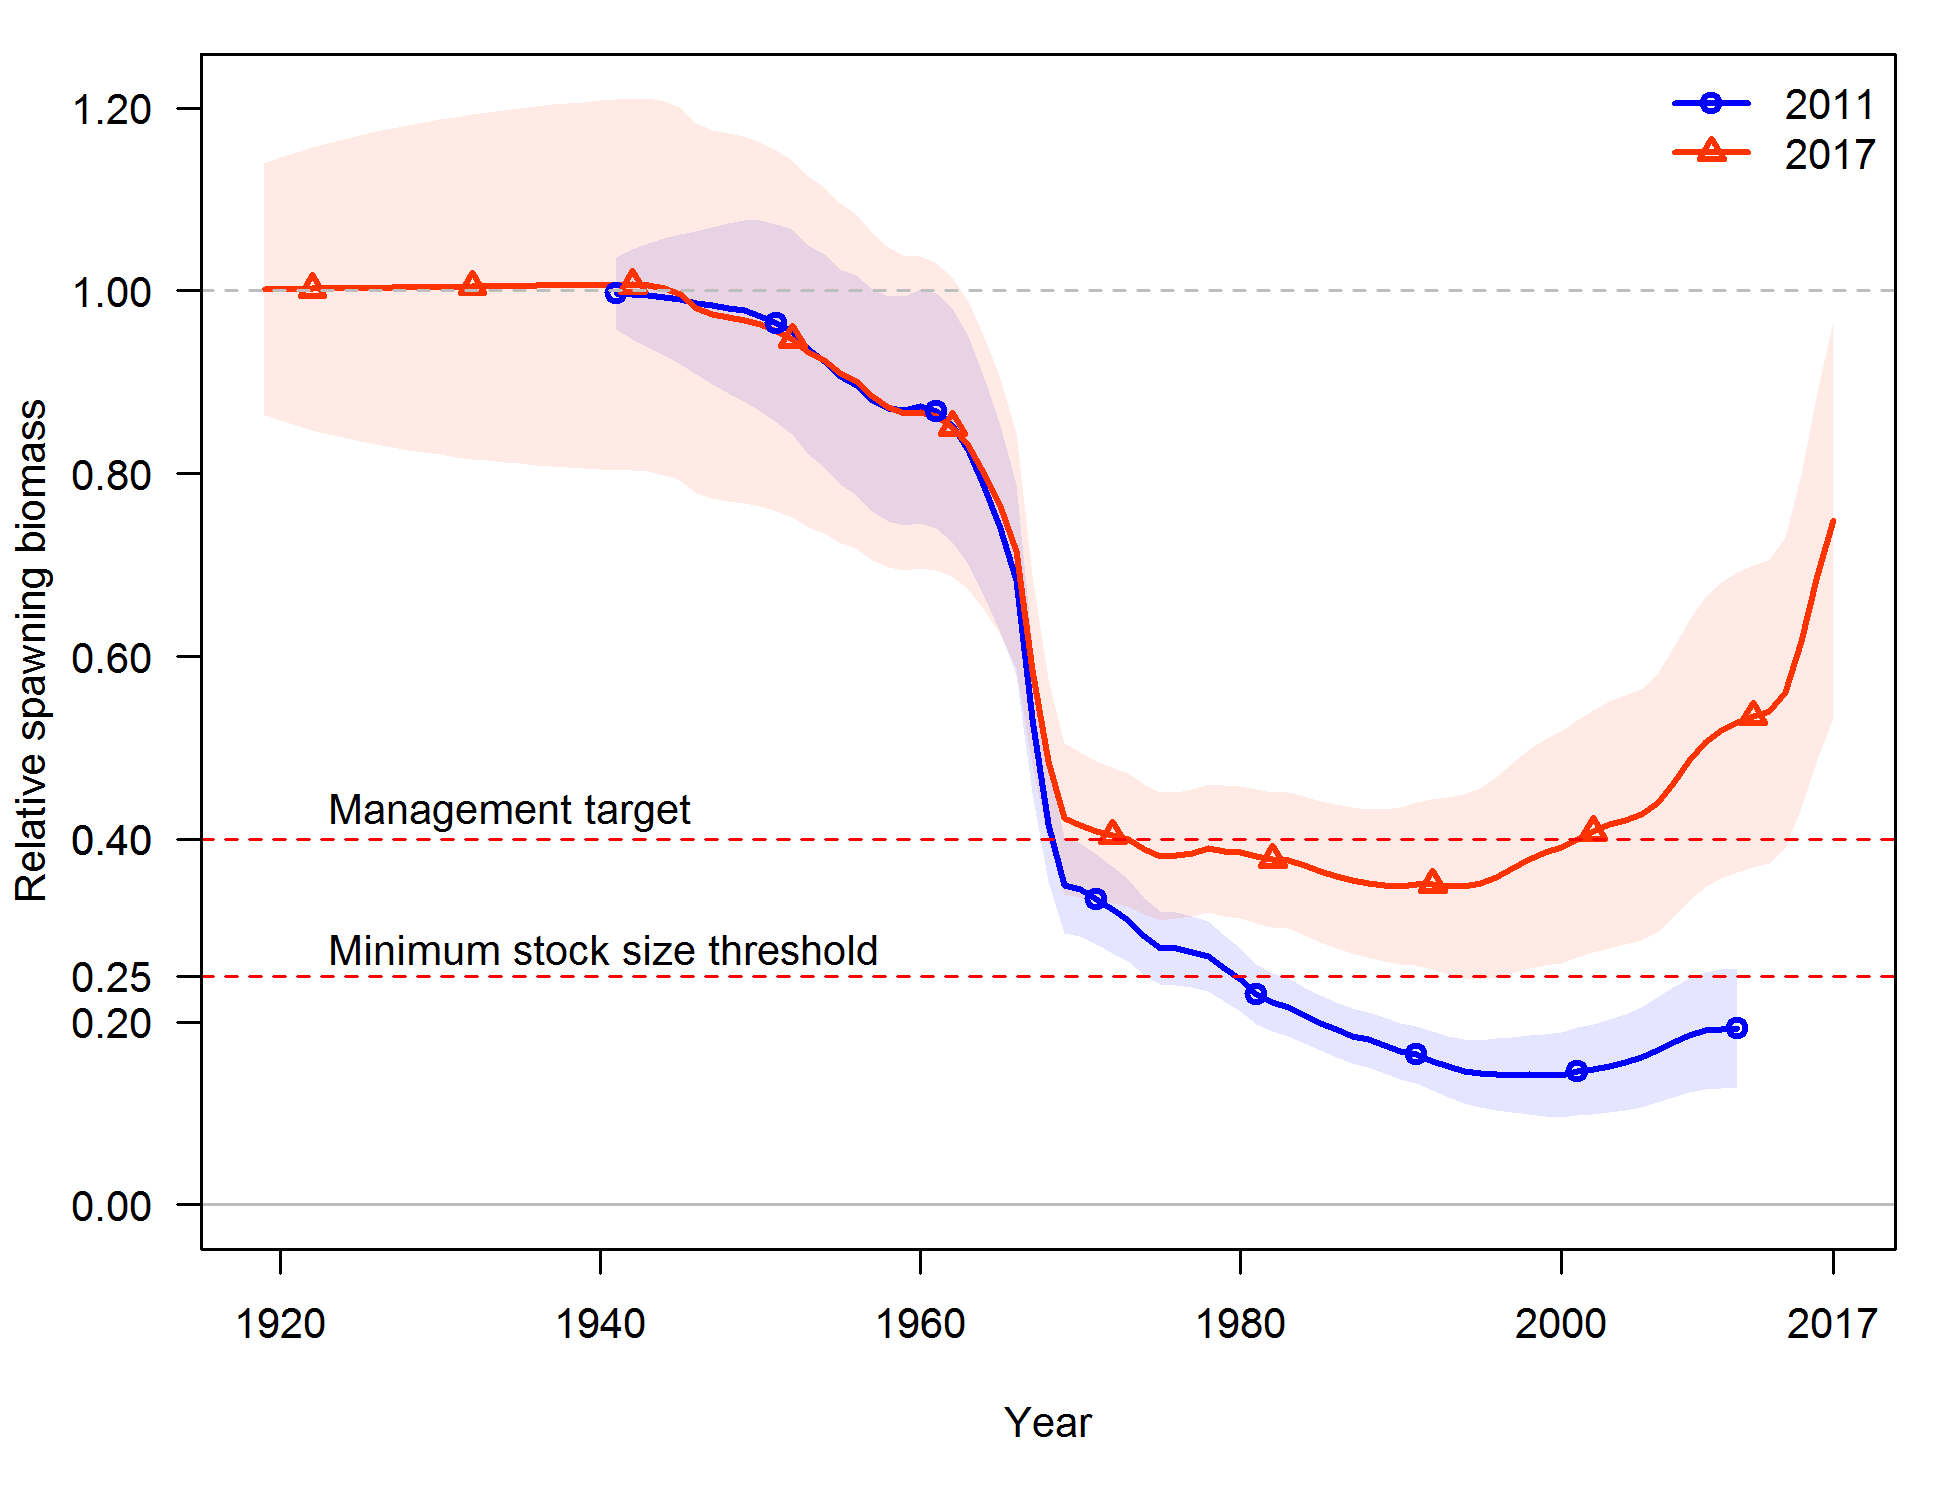
\includegraphics[scale = 0.50]{figures/2011_2017_Bratio.png}
  \end{center}
\end{frame}

\begin{frame}{Major Changes Between the Previous and Current Assessment}
  \begin{itemize}
    \item Steepness 
      %\begin{itemize}
      %  \item The 2011 assessment assumed $h$ = 0.40
      %  \item Current assessment assumed $h$ = 0.50. 
      %\end{itemize}
    \item Natural Mortality
      %\begin{itemize}
      %  \item 
      %\end{itemize}
    \item Landing History
    \item Maturity and Fecundity
    \item Fleet and Survey Selectivities 
      %\begin{itemize}
      %  \item Fishery and survey specific estimated in current assessment 
        %- 60.6\% fixed 73.1\% estimated
      %\end{itemize}
  \end{itemize}
\end{frame}

\begin{frame}{2011 Model Data "Update"}
  \begin{itemize}
    \item Added layers of new data cumulatively while retaining 2011 modeling assumptions
  \end{itemize}
  \begin{center}
    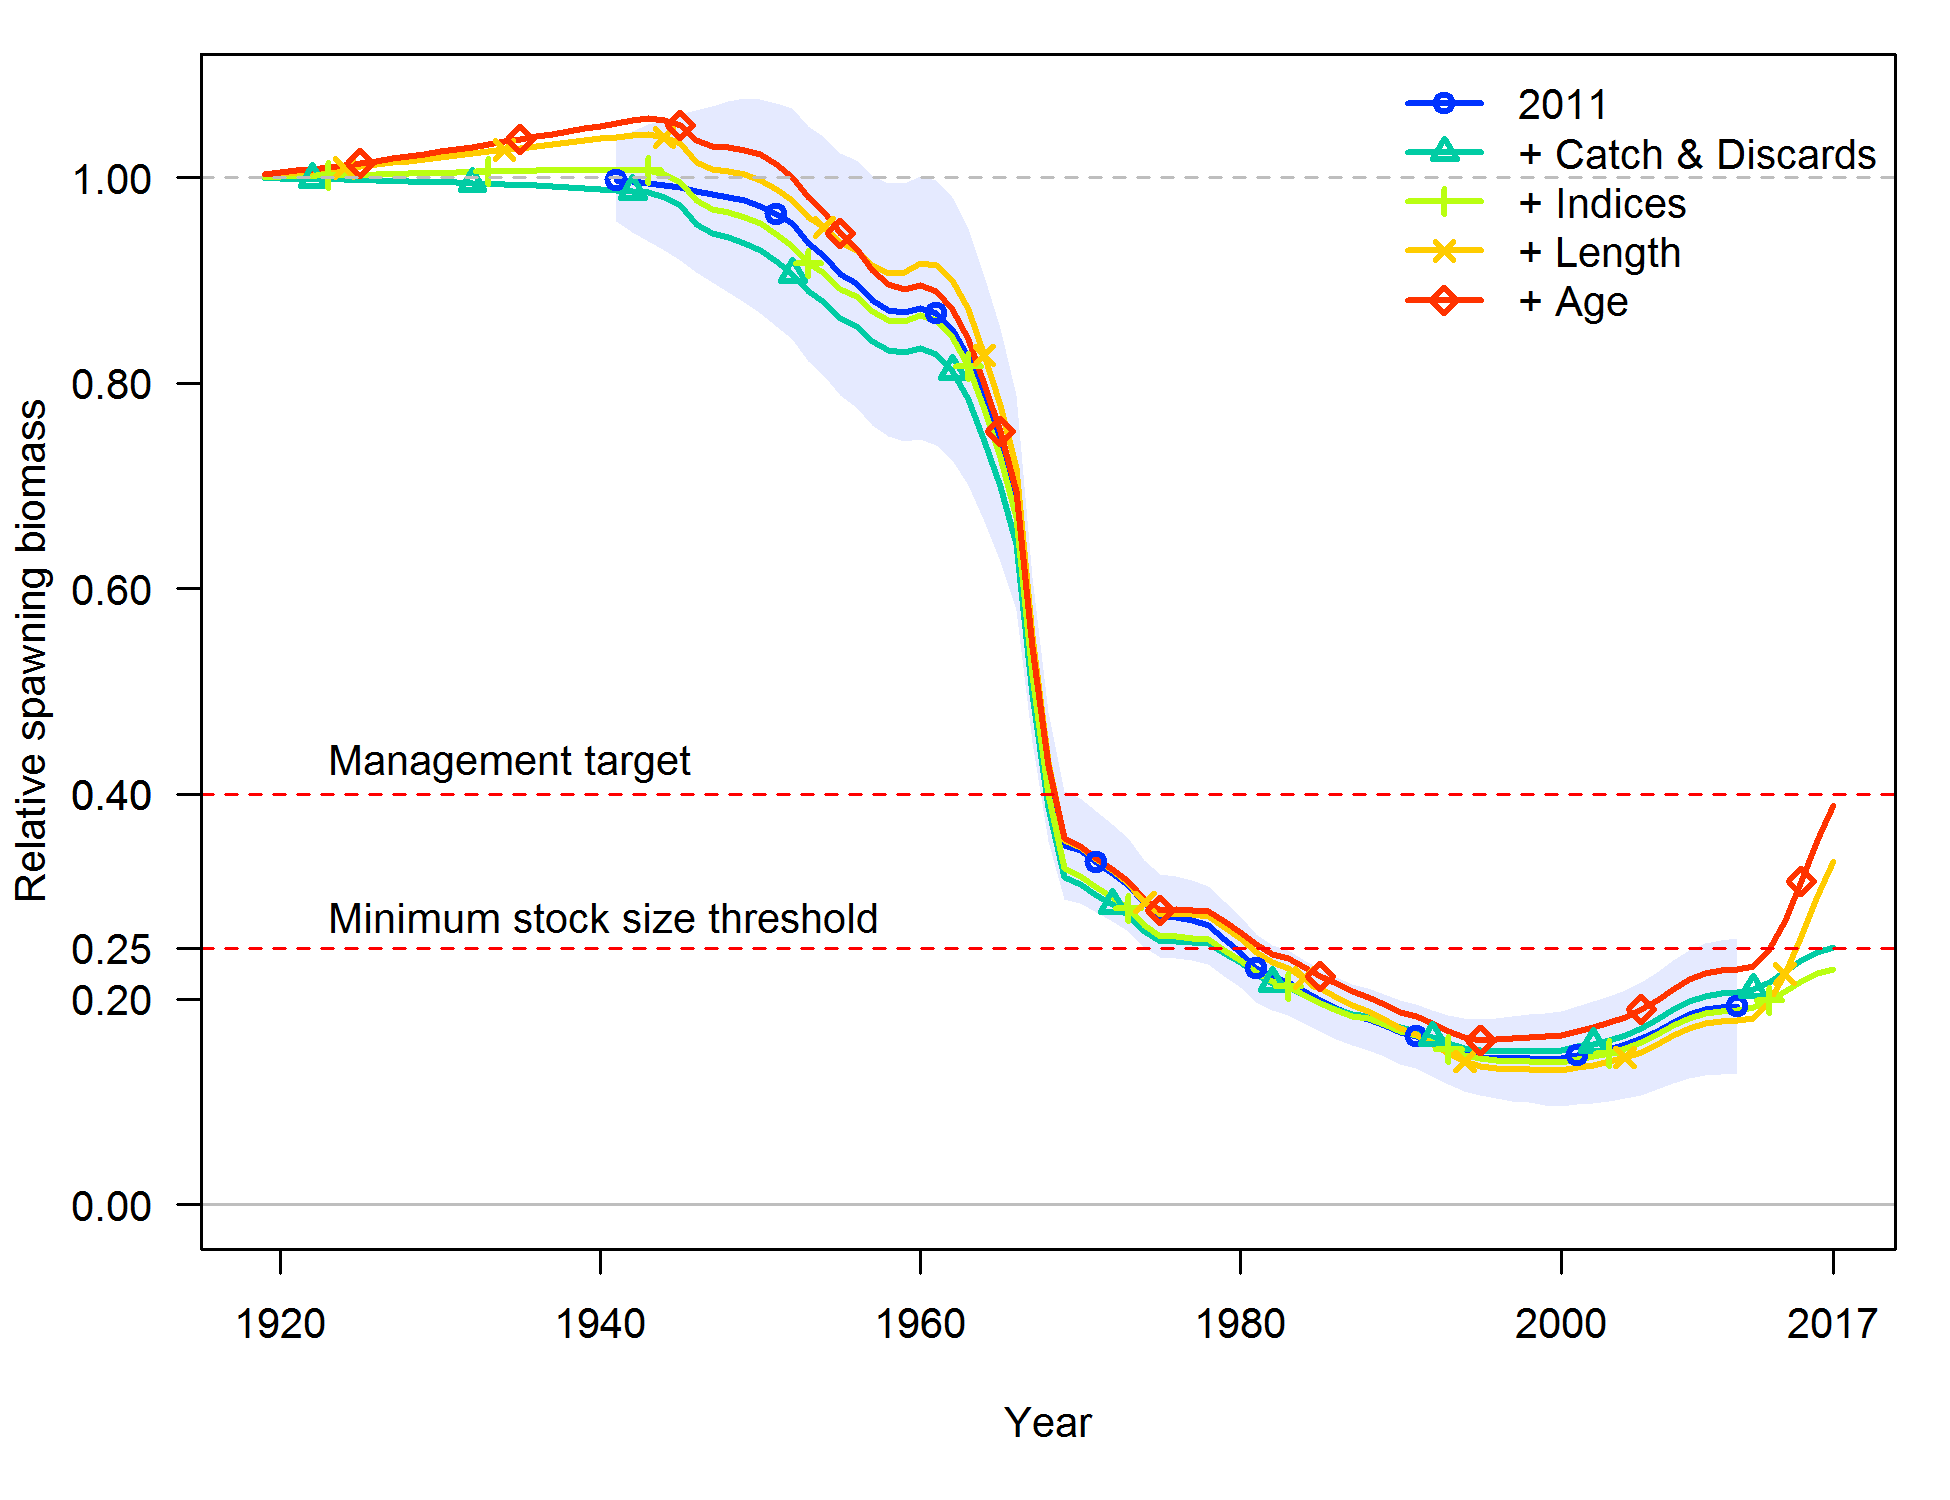
\includegraphics[scale = 0.42]{figures/Data_Bratio_uncertainty.png}
  \end{center}
\end{frame}

\begin{frame}{2017 Base Model Sensitivities}
  %\begin{center}
    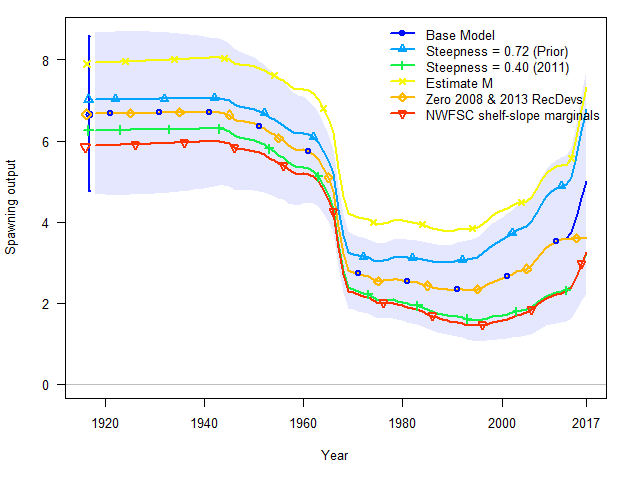
\includegraphics[scale = 0.28]{figures/SSB_sensitivities_1.png}
    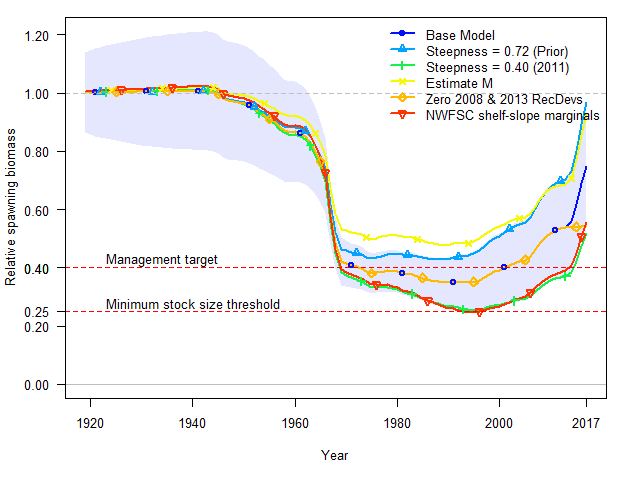
\includegraphics[scale = 0.28]{figures/Bratio_sensitivites_1.png}
  %\end{center}
\end{frame}

%\begin{frame}{Model Sensitivities - Relative}
%  \begin{center}
%    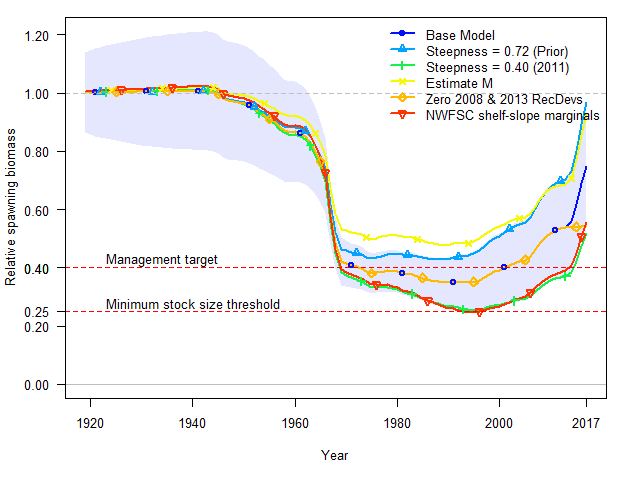
\includegraphics[scale = 0.40]{figures/Bratio_sensitivites_1.png}
%  \end{center}
%\end{frame}

%\begin{frame}{Model Sensitivities - Indices}
%  \begin{center}
%    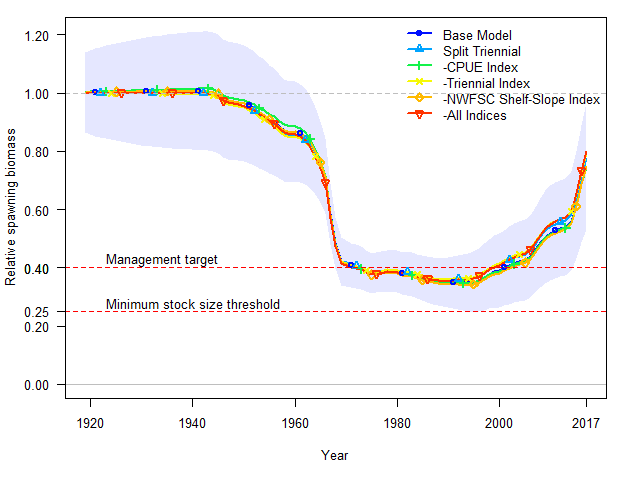
\includegraphics[scale = 0.40]{figures/Bratio_indices.png}
%  \end{center}
%\end{frame}

\subsection{Uncertainties}
\begin{frame}{Key Sources of Uncertainty}
  \begin{itemize}
    \item Steepness
    \begin{itemize}
      \item Fixed at 0.50 within the base model.  Likelihood profile over steepness indicates no information in data concerning steepness.  Fixing the value at the steepness prior value of 0.72 results in stock status 97\% of unfished.
    \end{itemize}
    \item Natural Mortality
      \begin{itemize}
        \item Fixed at 0.054 for males and females, the mean of the prior when maximum age is 100.  Likelihood profile relatively flat around the prior.
      \end{itemize}
    \item Recruitment 
      \begin{itemize} 
        \item Estimated large recruitments in 2008 and 2013. 
        \item Setting these recruitments equal to the stock-recruitment curve results in a decline in stock status to ~54\%.
      \end{itemize}
    \item{NWFSC shelf-slope age data}
      \begin{itemize}
        \item Treating these data as either conditional age-at-length or as marginals results in differing estimates of $R_0$ and final stock status.
      \end{itemize}
  \end{itemize}
\end{frame}



%------------------------------------------------------------------------------------
\section{Biology}

%------------------------------------------------------------------------------------
\subsection{Overview}
\begin{frame}{Pacific ocean perch (\textit{Sebastes alutus})}
\begin{columns}
  \begin{column}{0.5\textwidth}
      \begin{itemize}
        \item Distributed from  Alaska Aleutian Islands to Northern California
        \item Typically disctributed between 200 - 400 meters during summer months
        \item Semi-demersal and can be pelagic
        \item Both sexes move to deeper water with age
      \end{itemize}
  \end{column}
  
  \begin{column}{0.5\textwidth}
    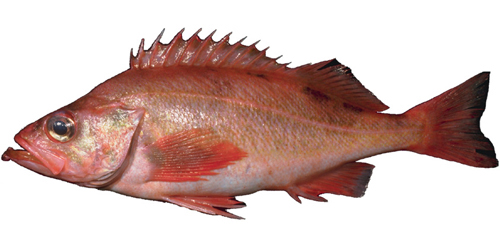
\includegraphics[scale = 0.25]{C:/Users/Chantel.Wetzel/Documents/GitHub/POP_2017/Sebastes_alutus.png}
    \begin{itemize}
        \item Females move to deeper waters post-spawning during winter months and return inshore in spring.
      \end{itemize}
  \end{column}
\end{columns}
\end{frame}


\subsection{Maturity}
\begin{frame}{Maturity}
\begin{columns}
  \begin{column}{0.55\textwidth}
      Functional maturity-at-length
      \begin{itemize}
        \item Categorized mature and immature fish based on the proportion of vitellogenin in the cytoplasm and atretic cells
        \item 50\% maturity is at larger lengths vs. biological maturity
        \item functional 50\% = 32.1 cm vs. biological 50\% = 30.1 cm
      \end{itemize}
  \end{column}
  
  \begin{column}{0.45\textwidth}
  \begin{center}
    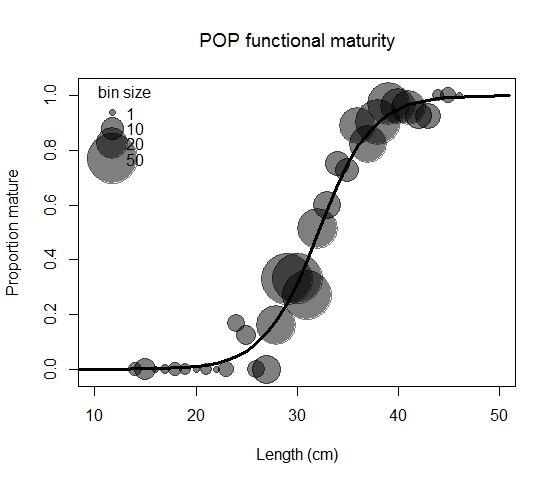
\includegraphics[scale = 0.40]{figures/Functional_Maturity.png}
  \end{center}
  \end{column}
\end{columns}
\end{frame}

\begin{frame}{Maturity Comparison}
  \begin{center}
    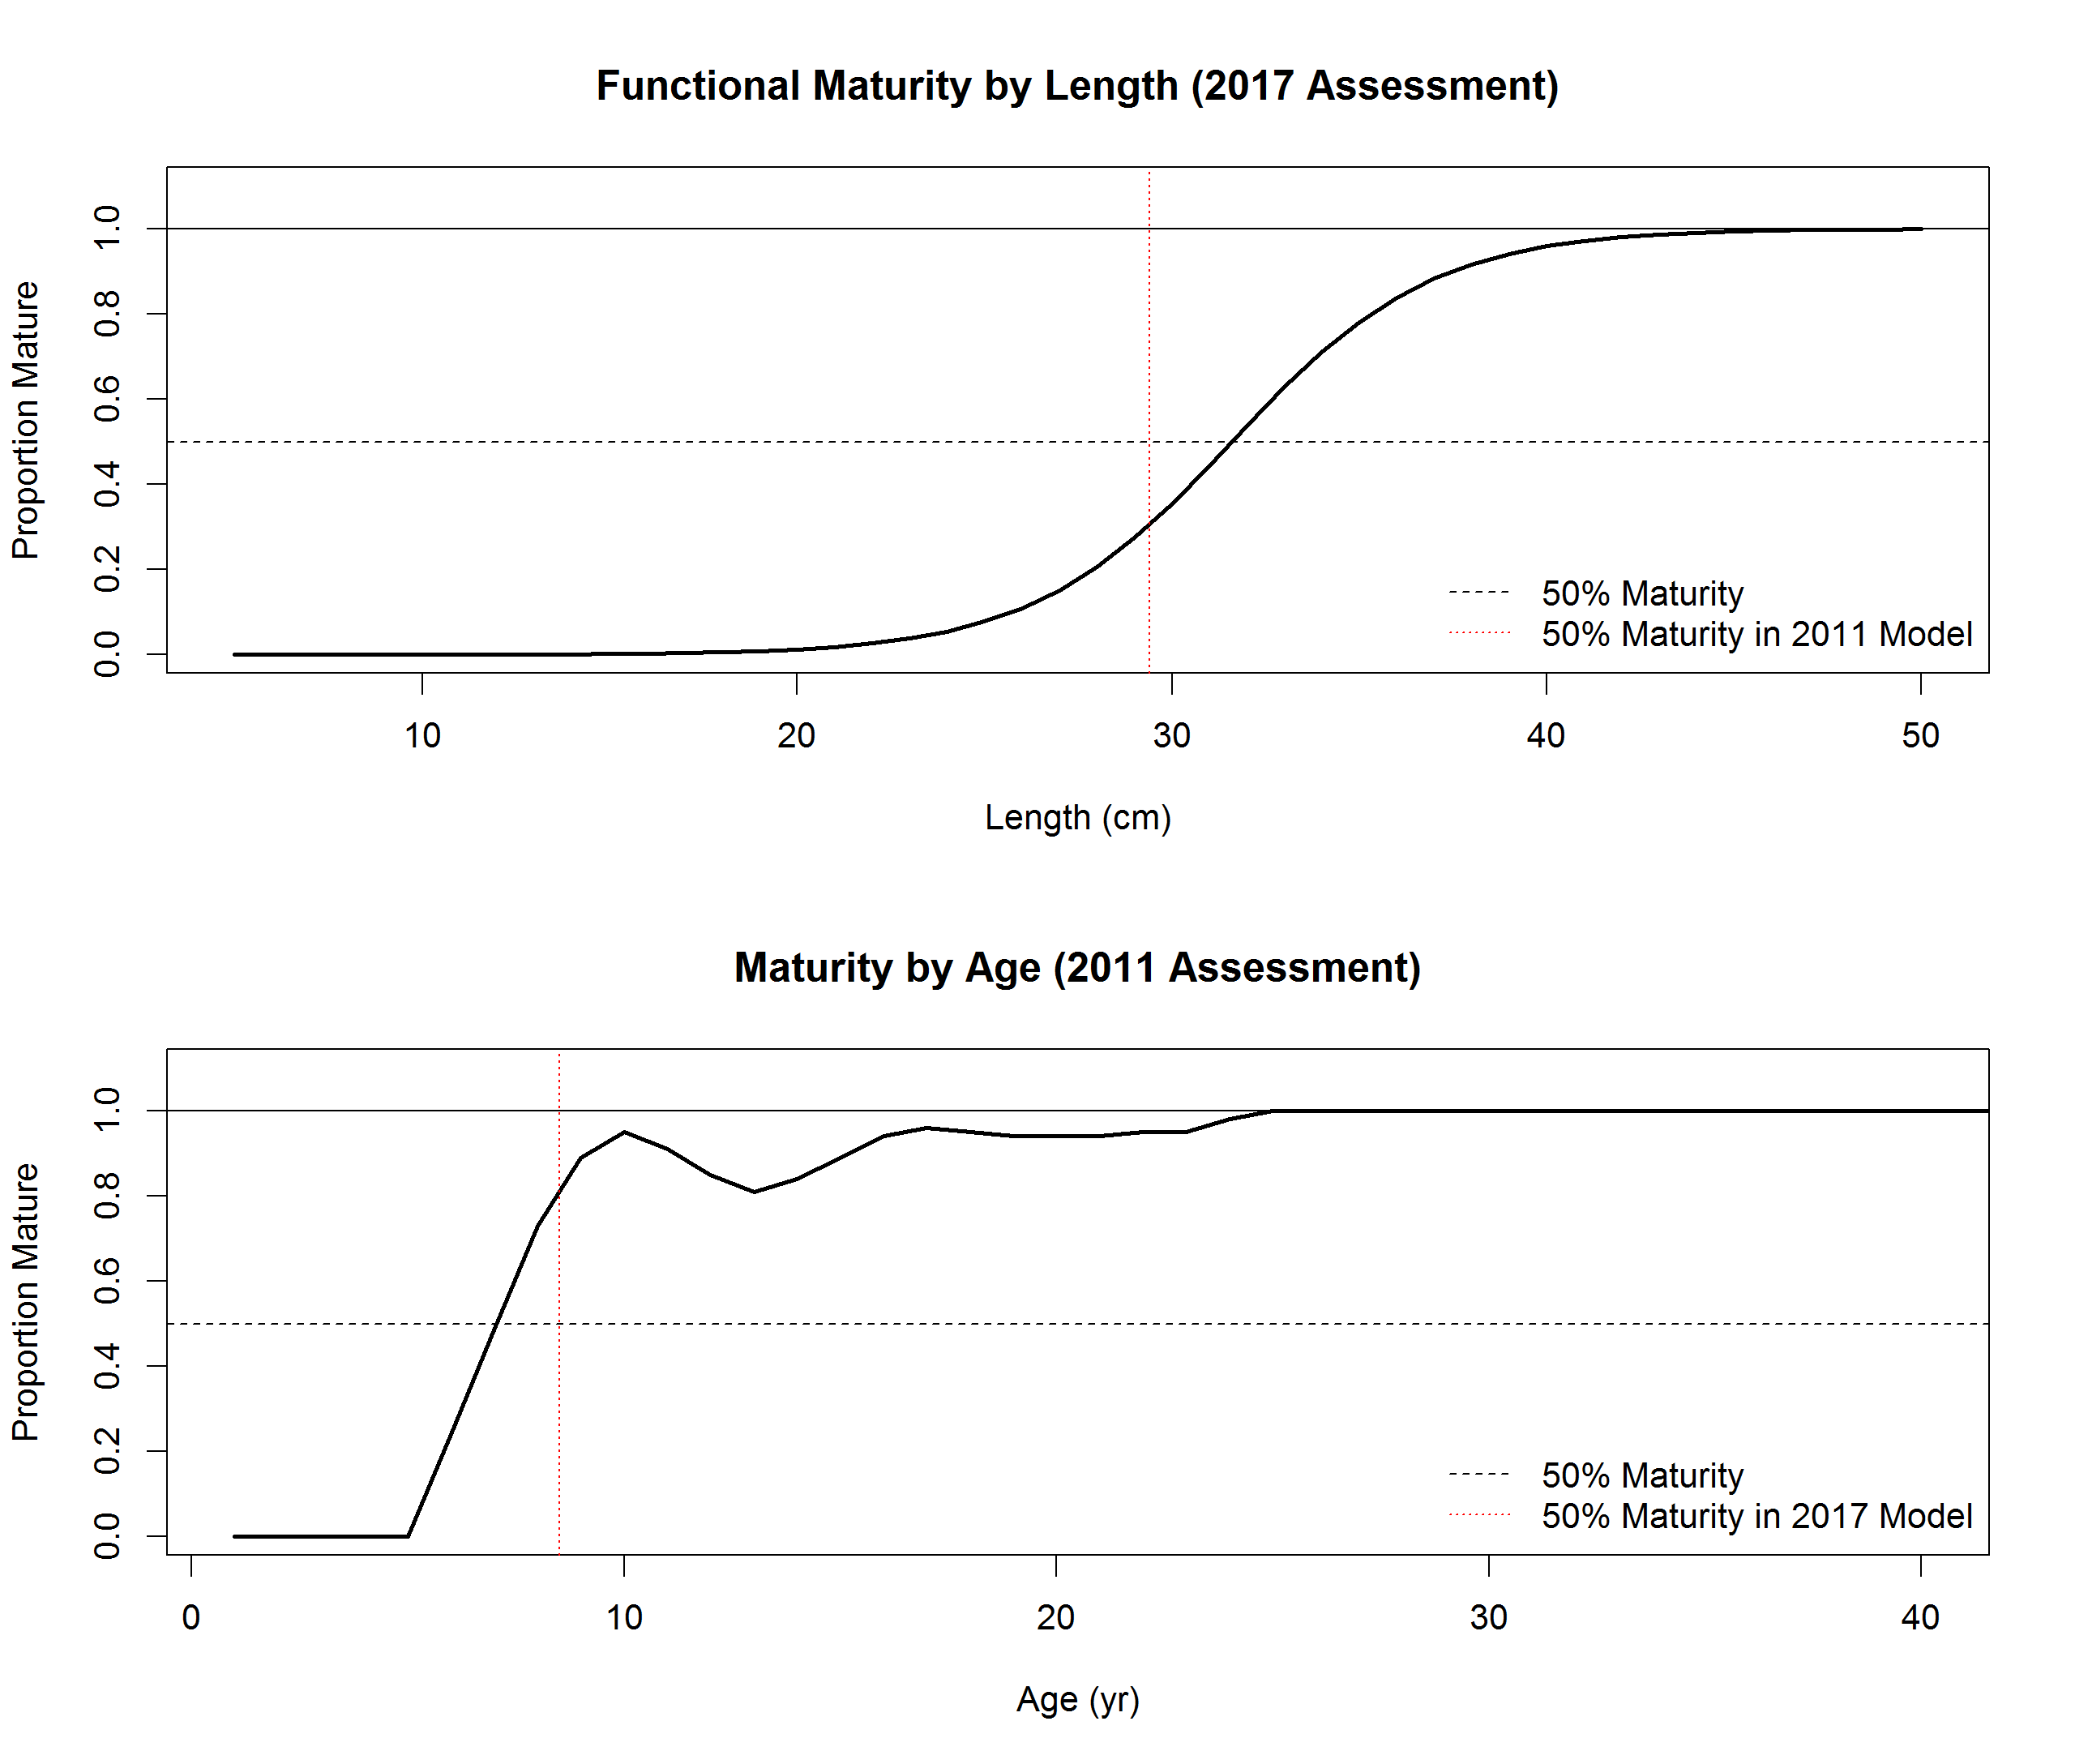
\includegraphics[scale = 0.3]{figures/Maturity_Comparison.png}
  \end{center}
  *Sensitivity to assumed maturity shown to not have a large impact on results
\end{frame}

\subsection{Fecundity}
\begin{frame}{Fecundity}
  \begin{center}
    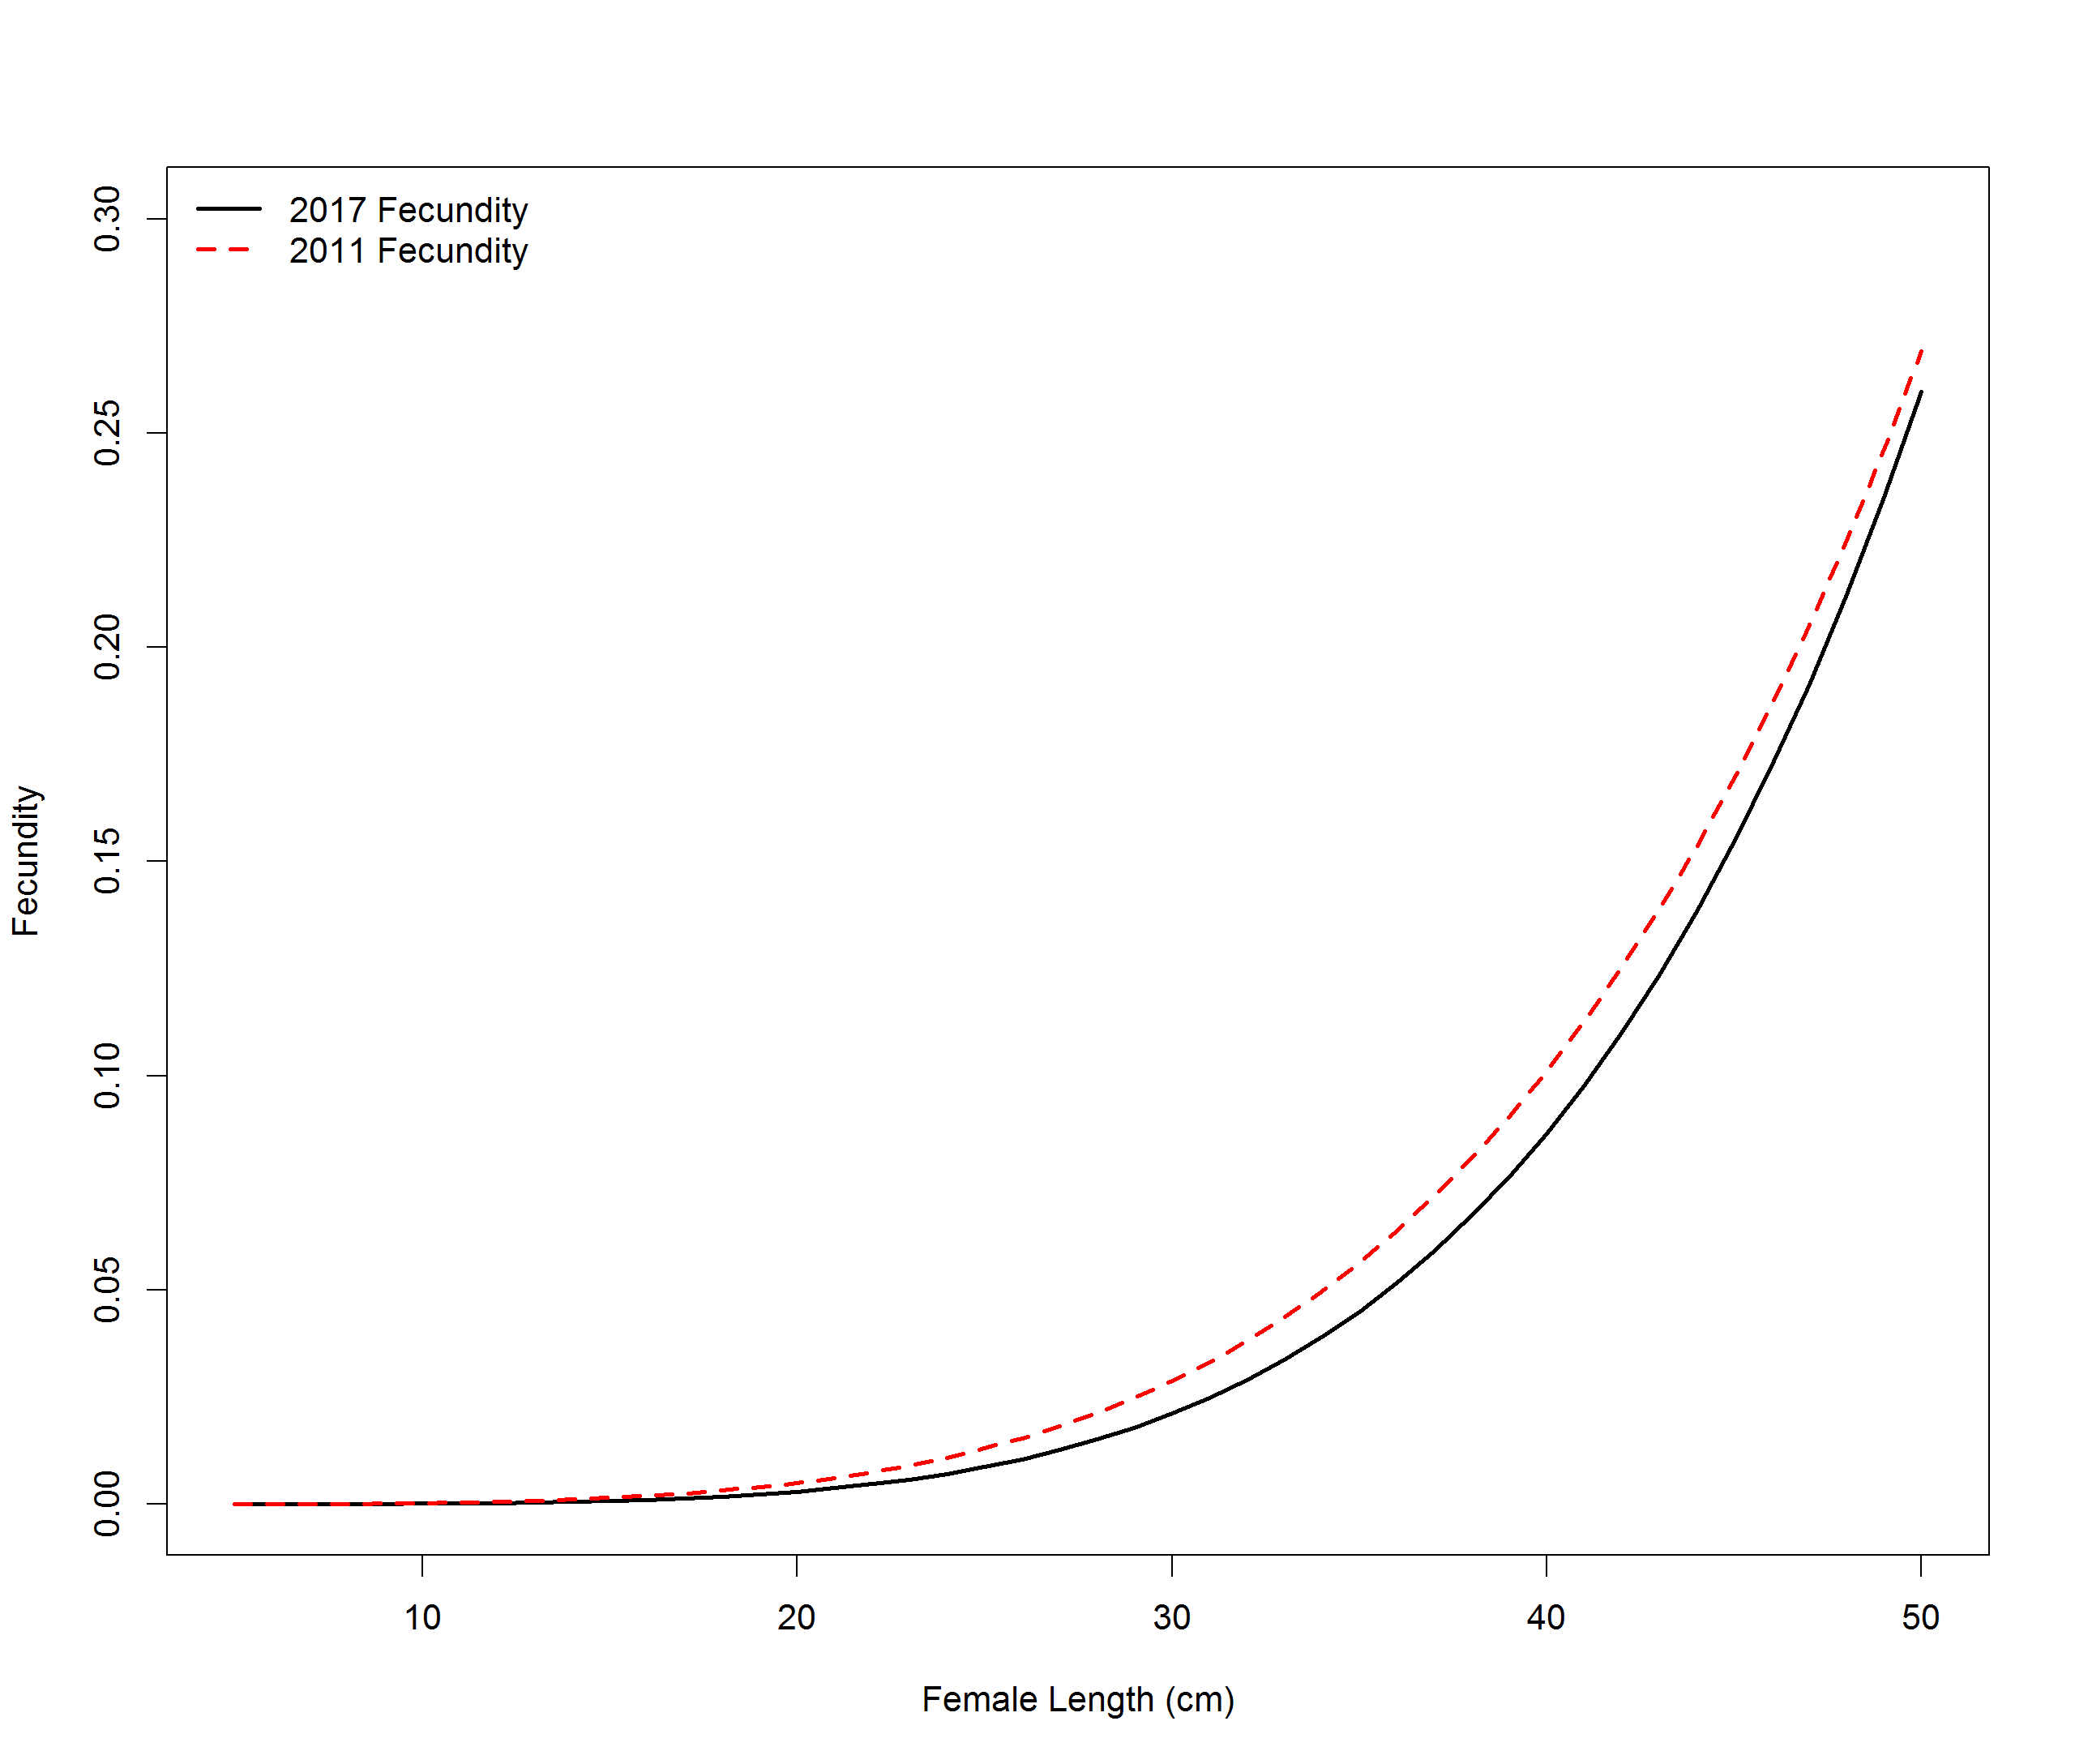
\includegraphics[scale = 0.3, trim={0, 0, 1cm, 1cm}, clip]{figures/Fecundity_Comparison.png}
  \end{center}
  *Sensitivity to assumed fecundity shown to not have a large impact on results
\end{frame}

\subsection{Growth}
\begin{frame}{Weight-at-length}
  \begin{center}
    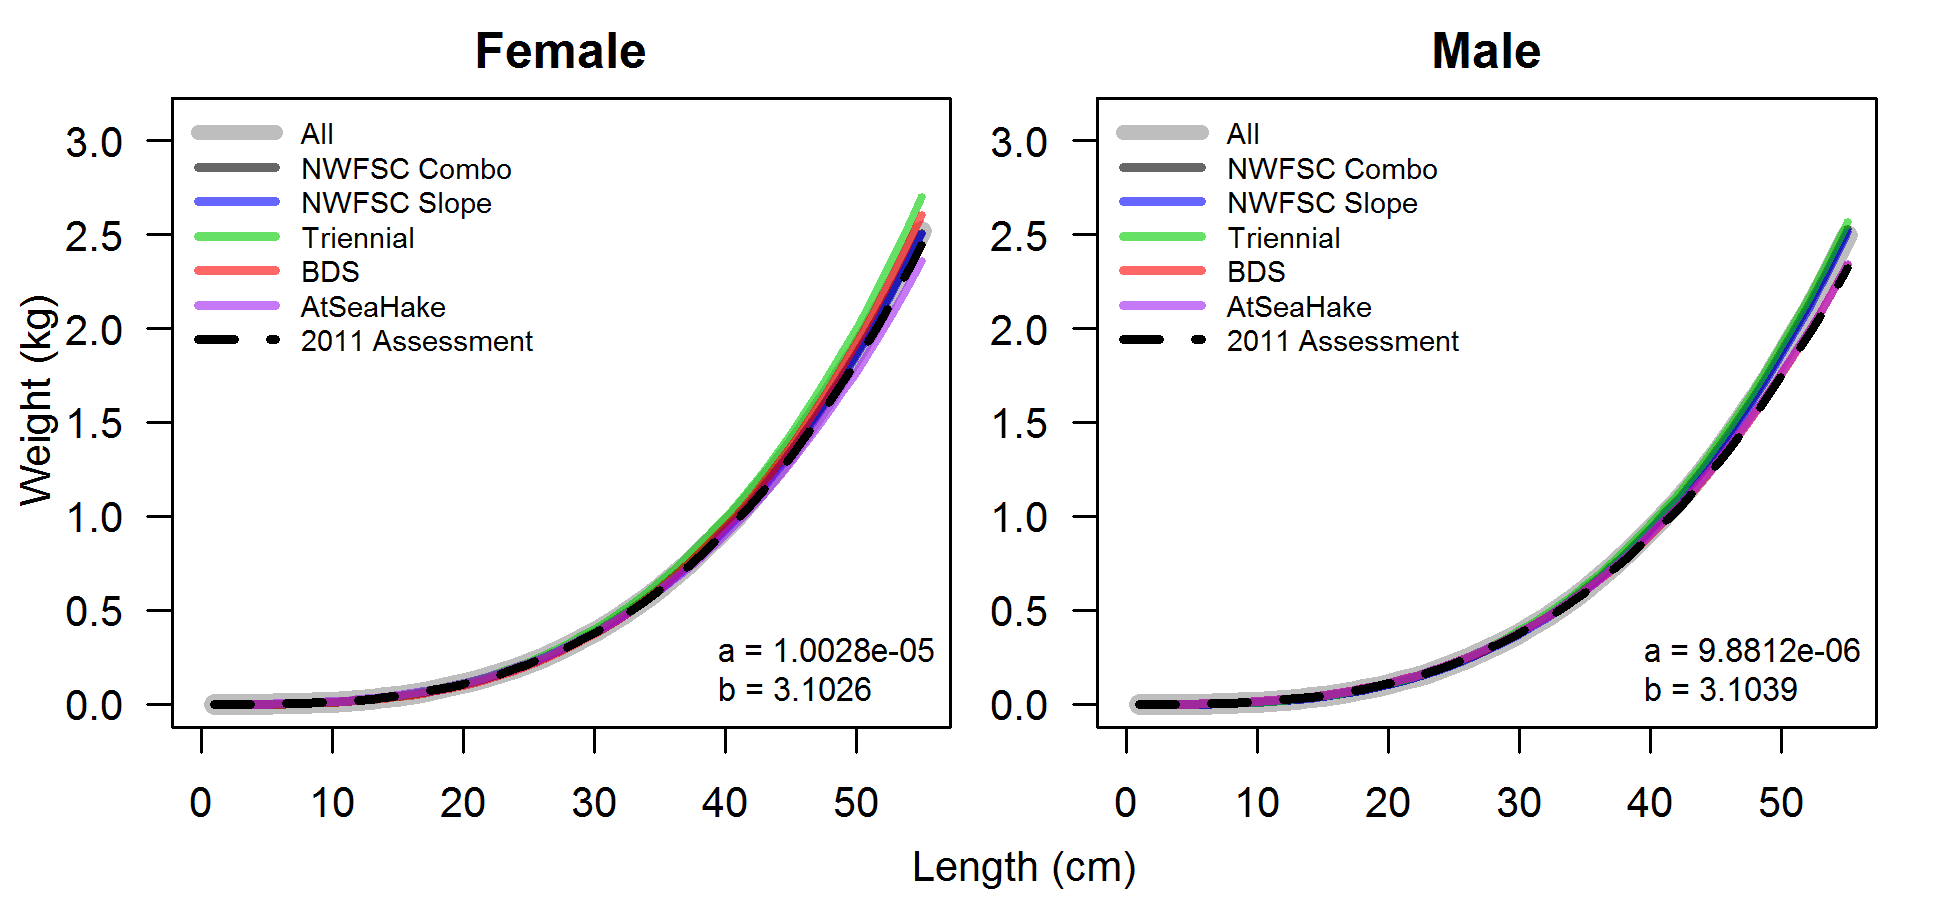
\includegraphics[scale = 0.75]{figures/weightAtLengthPred.png}
  \end{center}
\end{frame}

\begin{frame}{Length-at-age}
  \begin{center}
  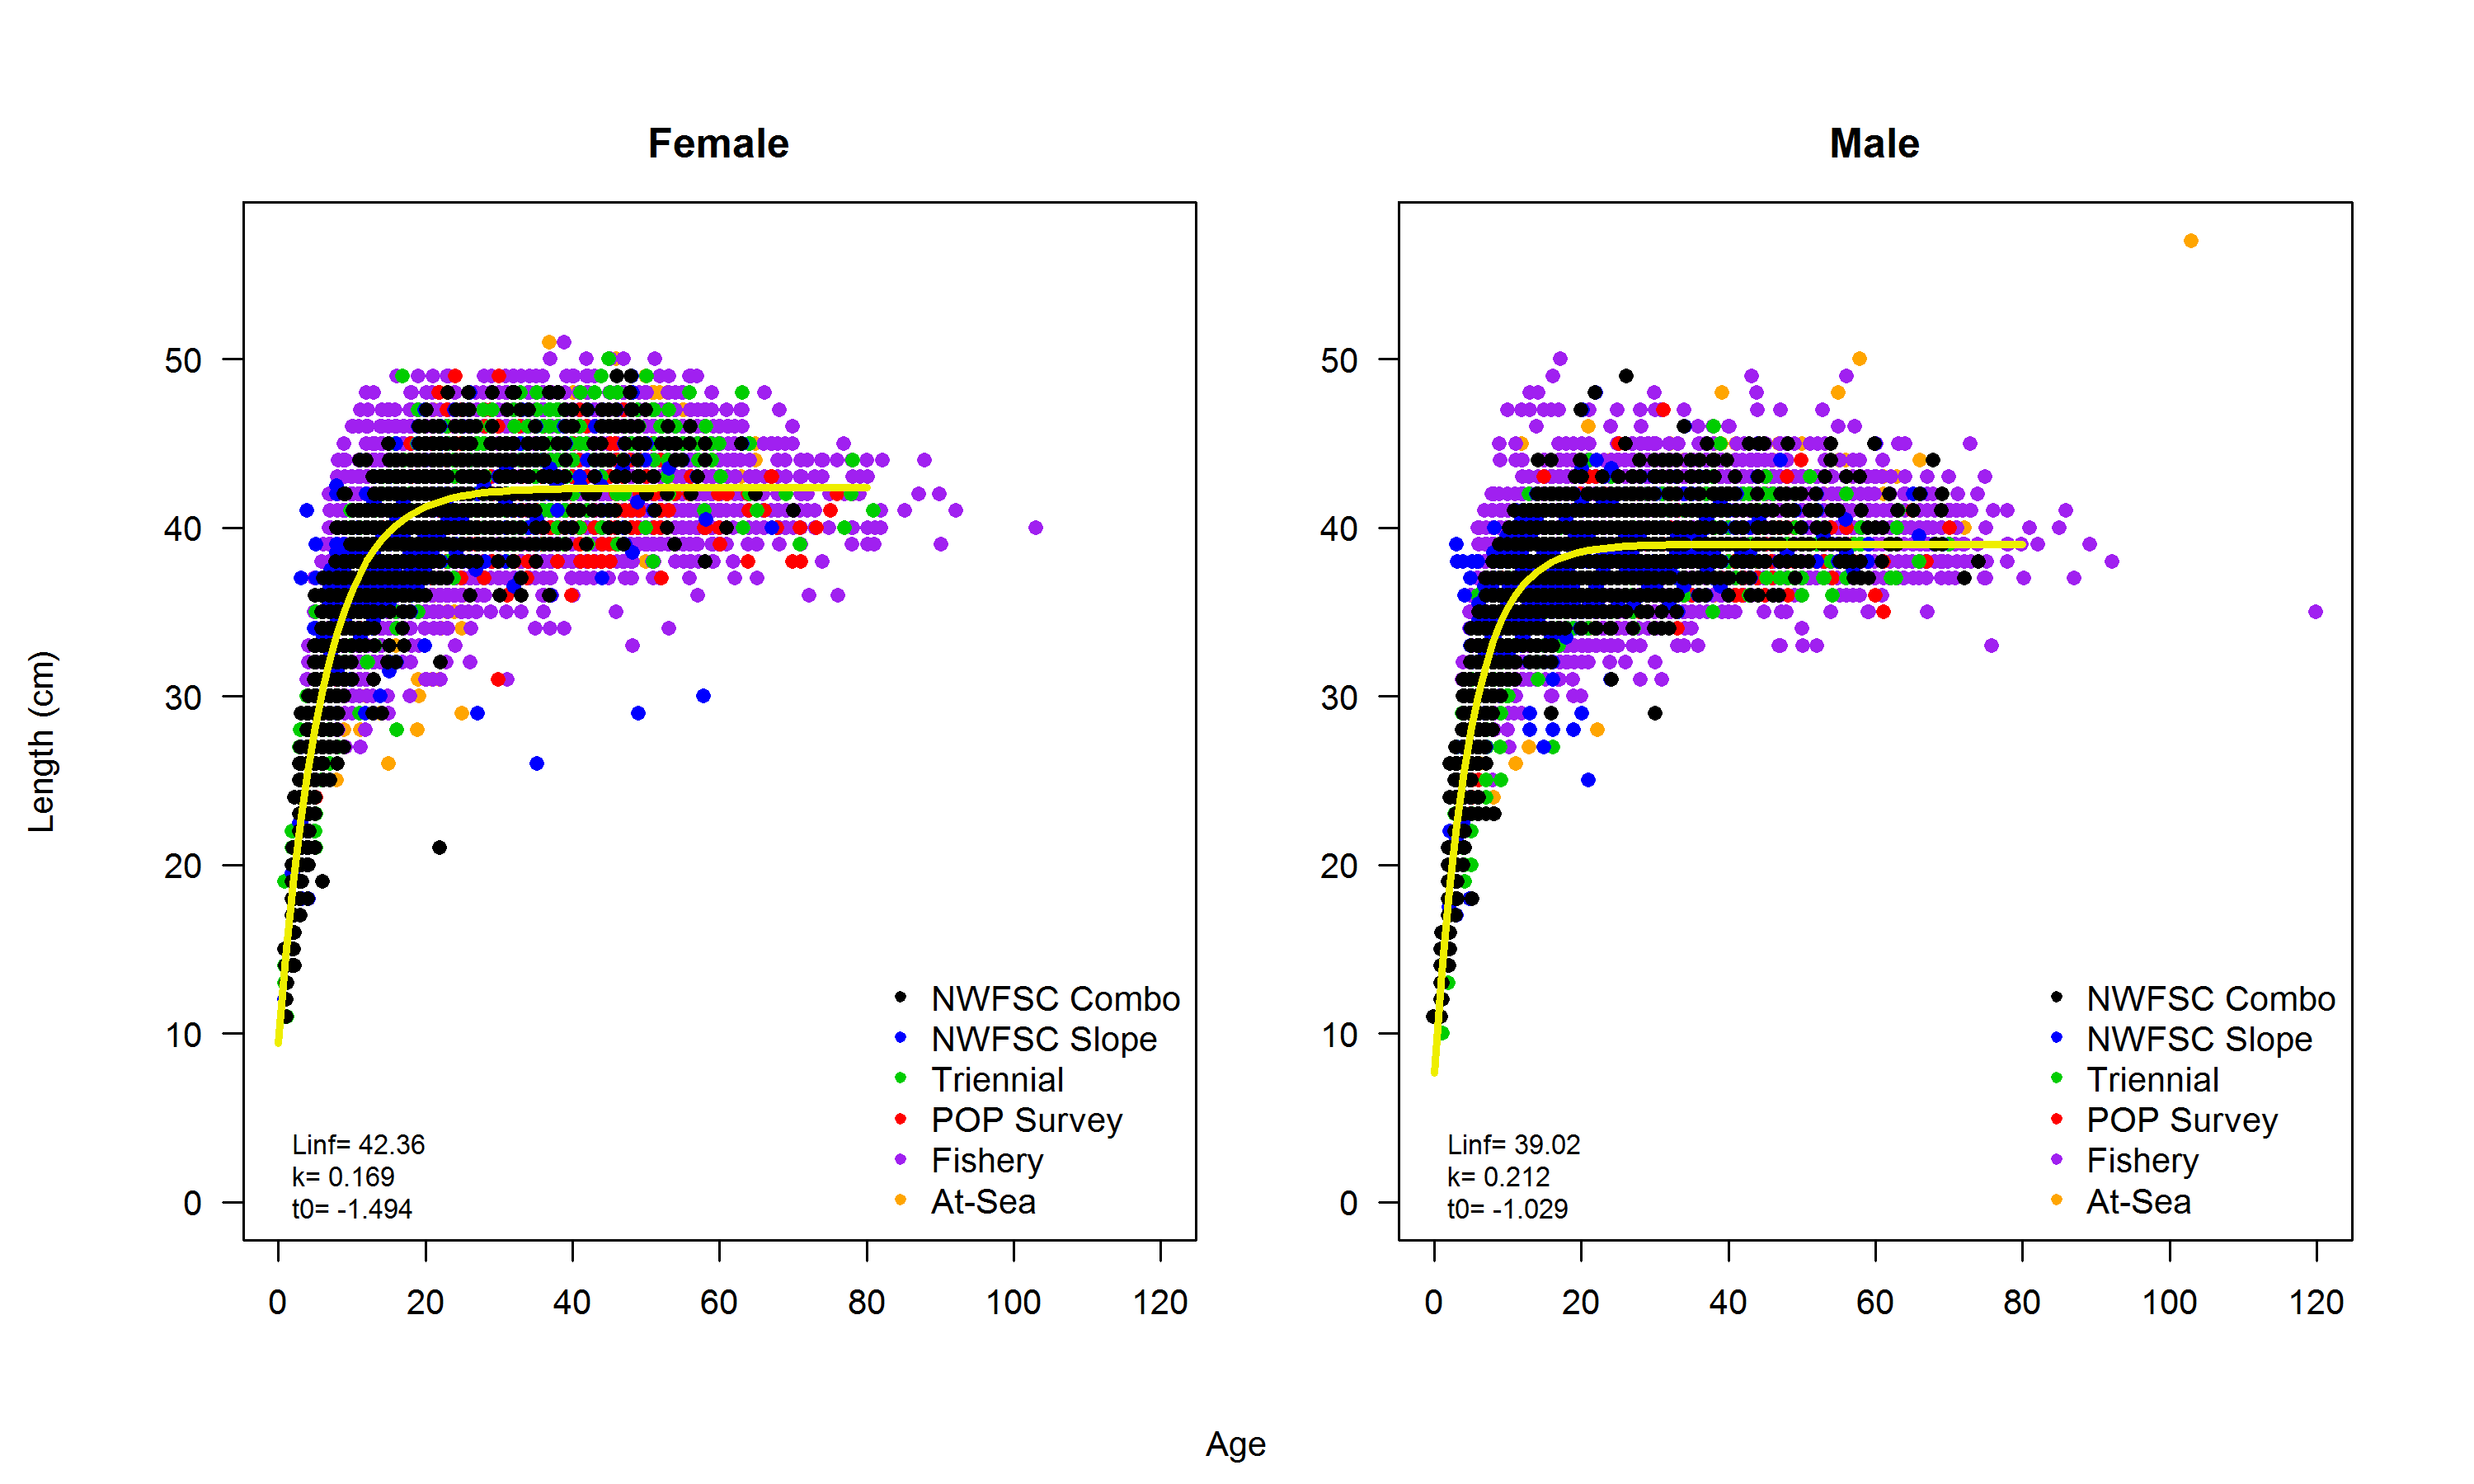
\includegraphics[scale = 0.45]{figures/LengthAgeAll_2.png}
  \end{center}
\end{frame}


\begin{frame}{Observed Ages}
  \begin{columns}
    \begin{column}{0.35\textwidth}
      \begin{itemize}
      \item Oldest age: 120 by the fishery (2007)
      \item Next oldest fish range from 90-103 collected by the fishery or the at-sea hake fishery between 1981-2010
      \end{itemize}
    \end{column}
    \begin{column}{0.65\textwidth}
      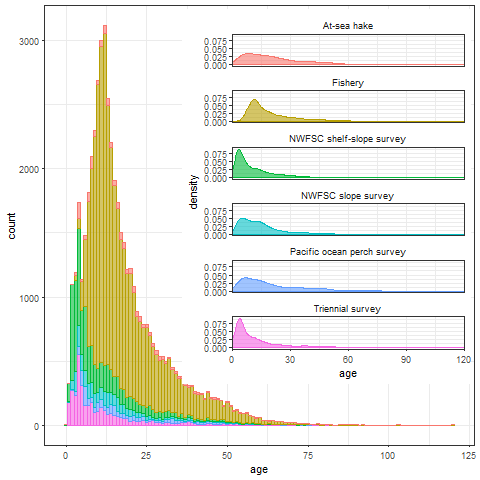
\includegraphics[scale = 0.45]{figures/pop2017_agesbysource.png}
    \end{column}
  \end{columns}
\end{frame}

%-------------------------------------------------------------------------------------
%\section{Data Summary}
%-------------------------------------------------------------------------------------

\subsection{}
\begin{frame}{Data Summary Used in the 2017 Assessment}
  \begin{figure}[ht]
    \begin{center}
      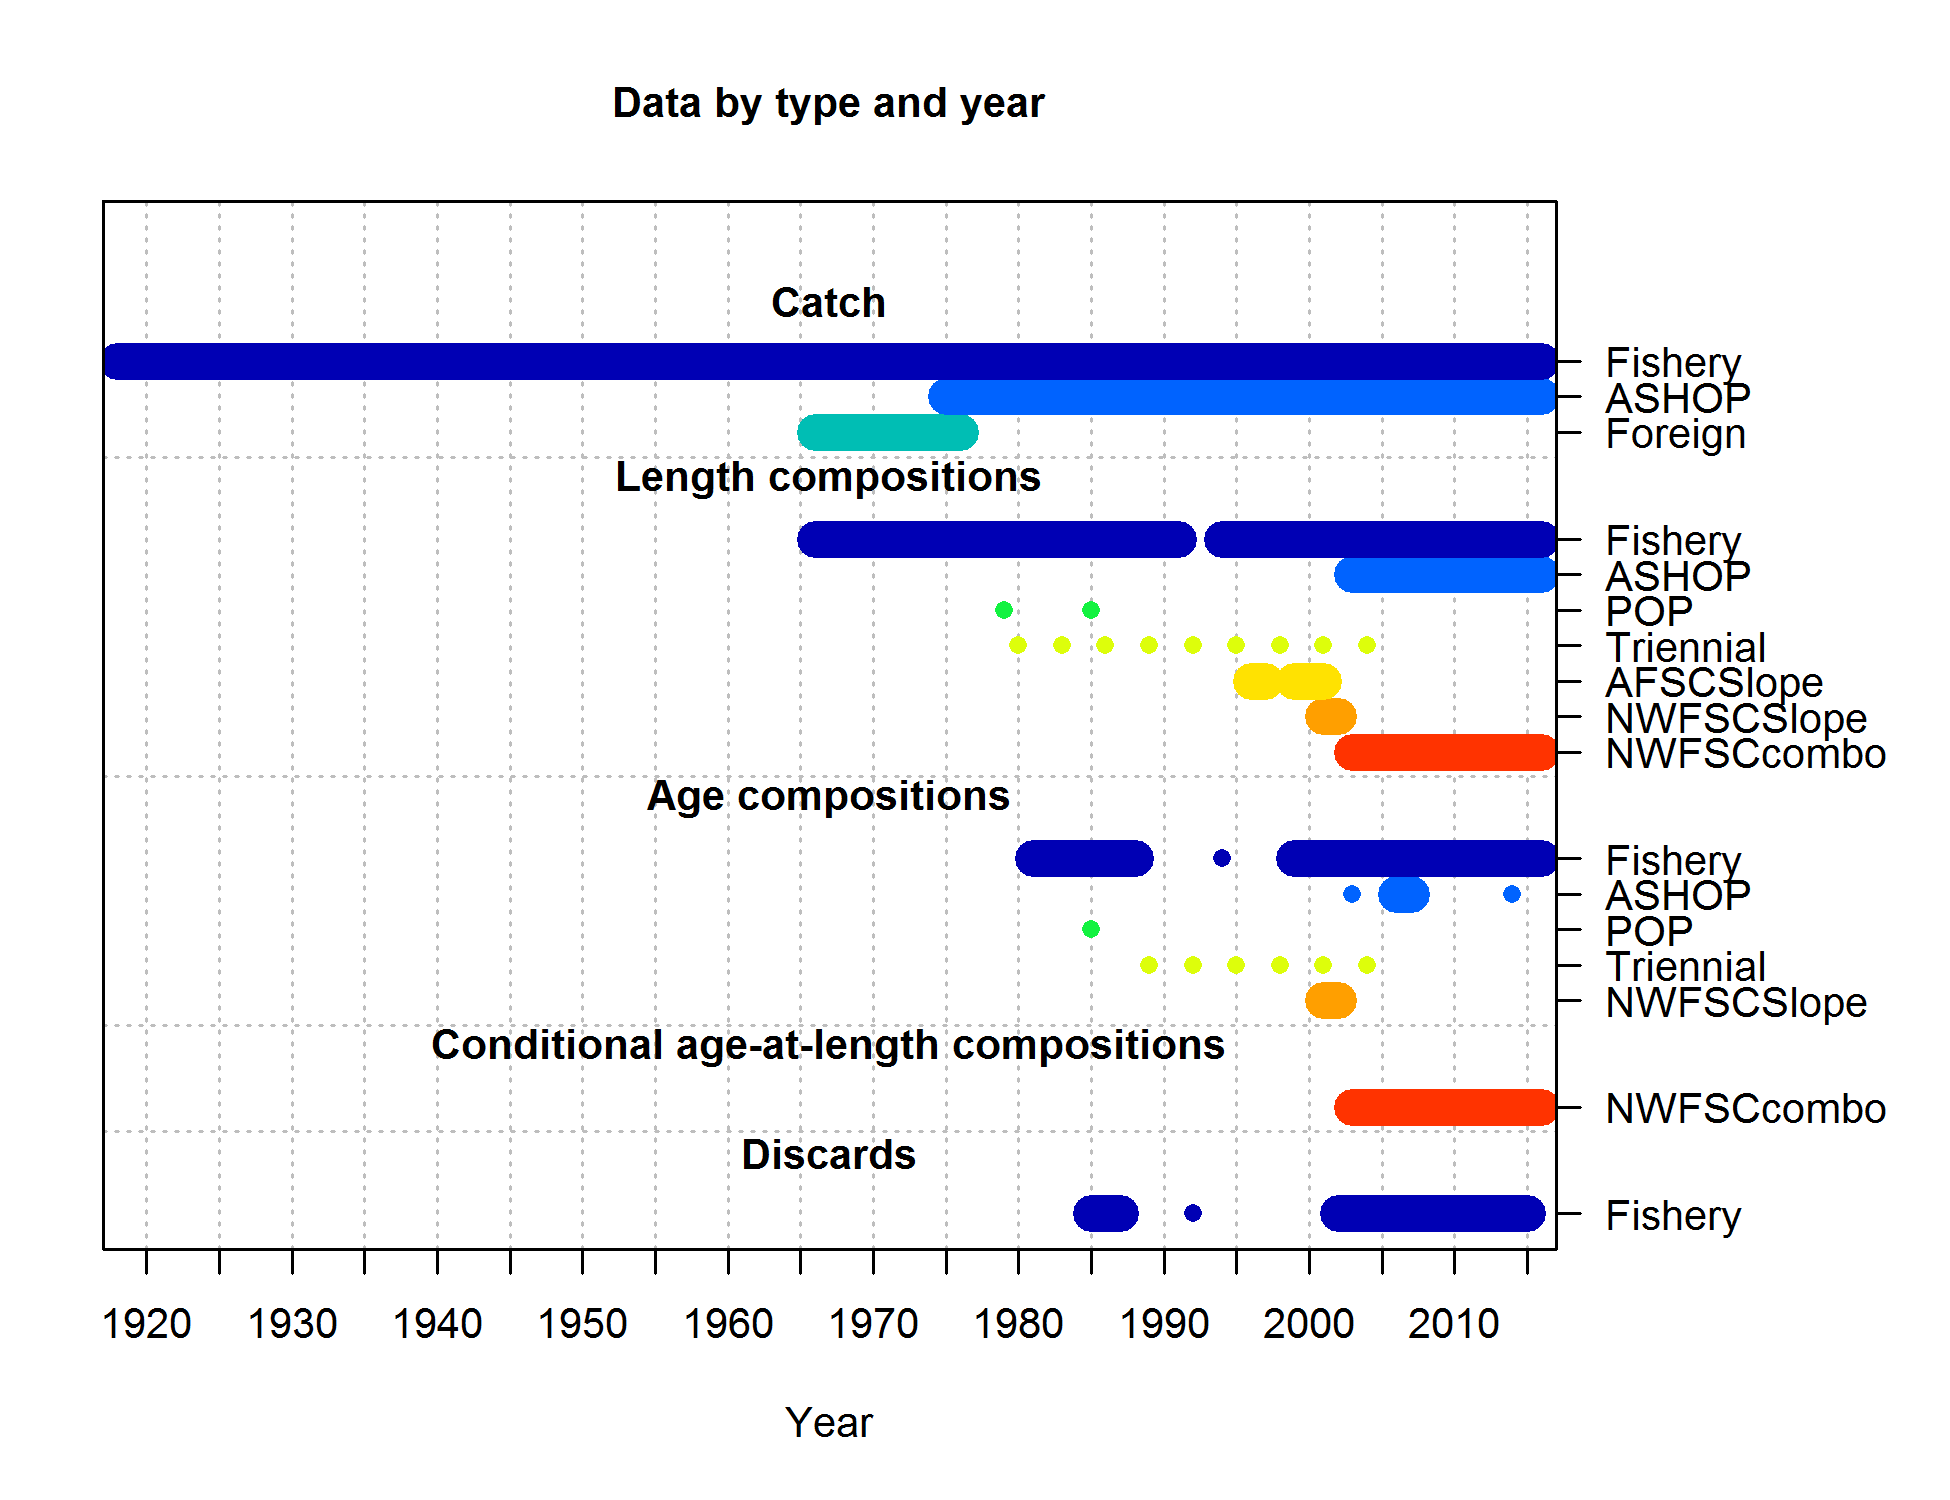
\includegraphics[height=3in]{r4ss/data_plot.png}

    \end{center}
  \end{figure}
\end{frame}


%---------------------------------------------------------------------------------
\section{Removals}
%---------------------------------------------------------------------------------
\subsection{Landings History by State}
\begin{frame}{Landings Data: 2017 vs. 2011}
  \begin{center}
    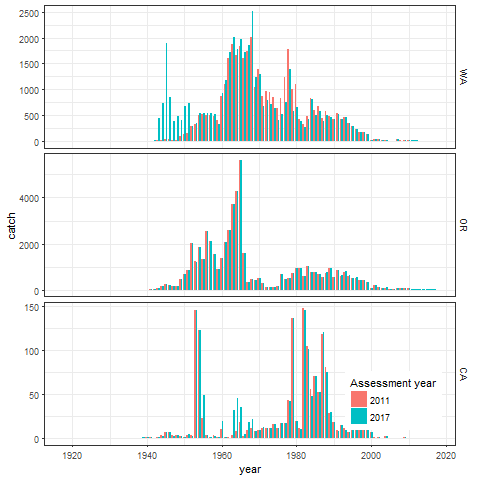
\includegraphics[scale = 0.45]{figures/pop2017_2011vs2017catches_states.png}
  \end{center}
\end{frame}

\begin{frame}{Cummalative Catch Difference}
  \begin{center}
    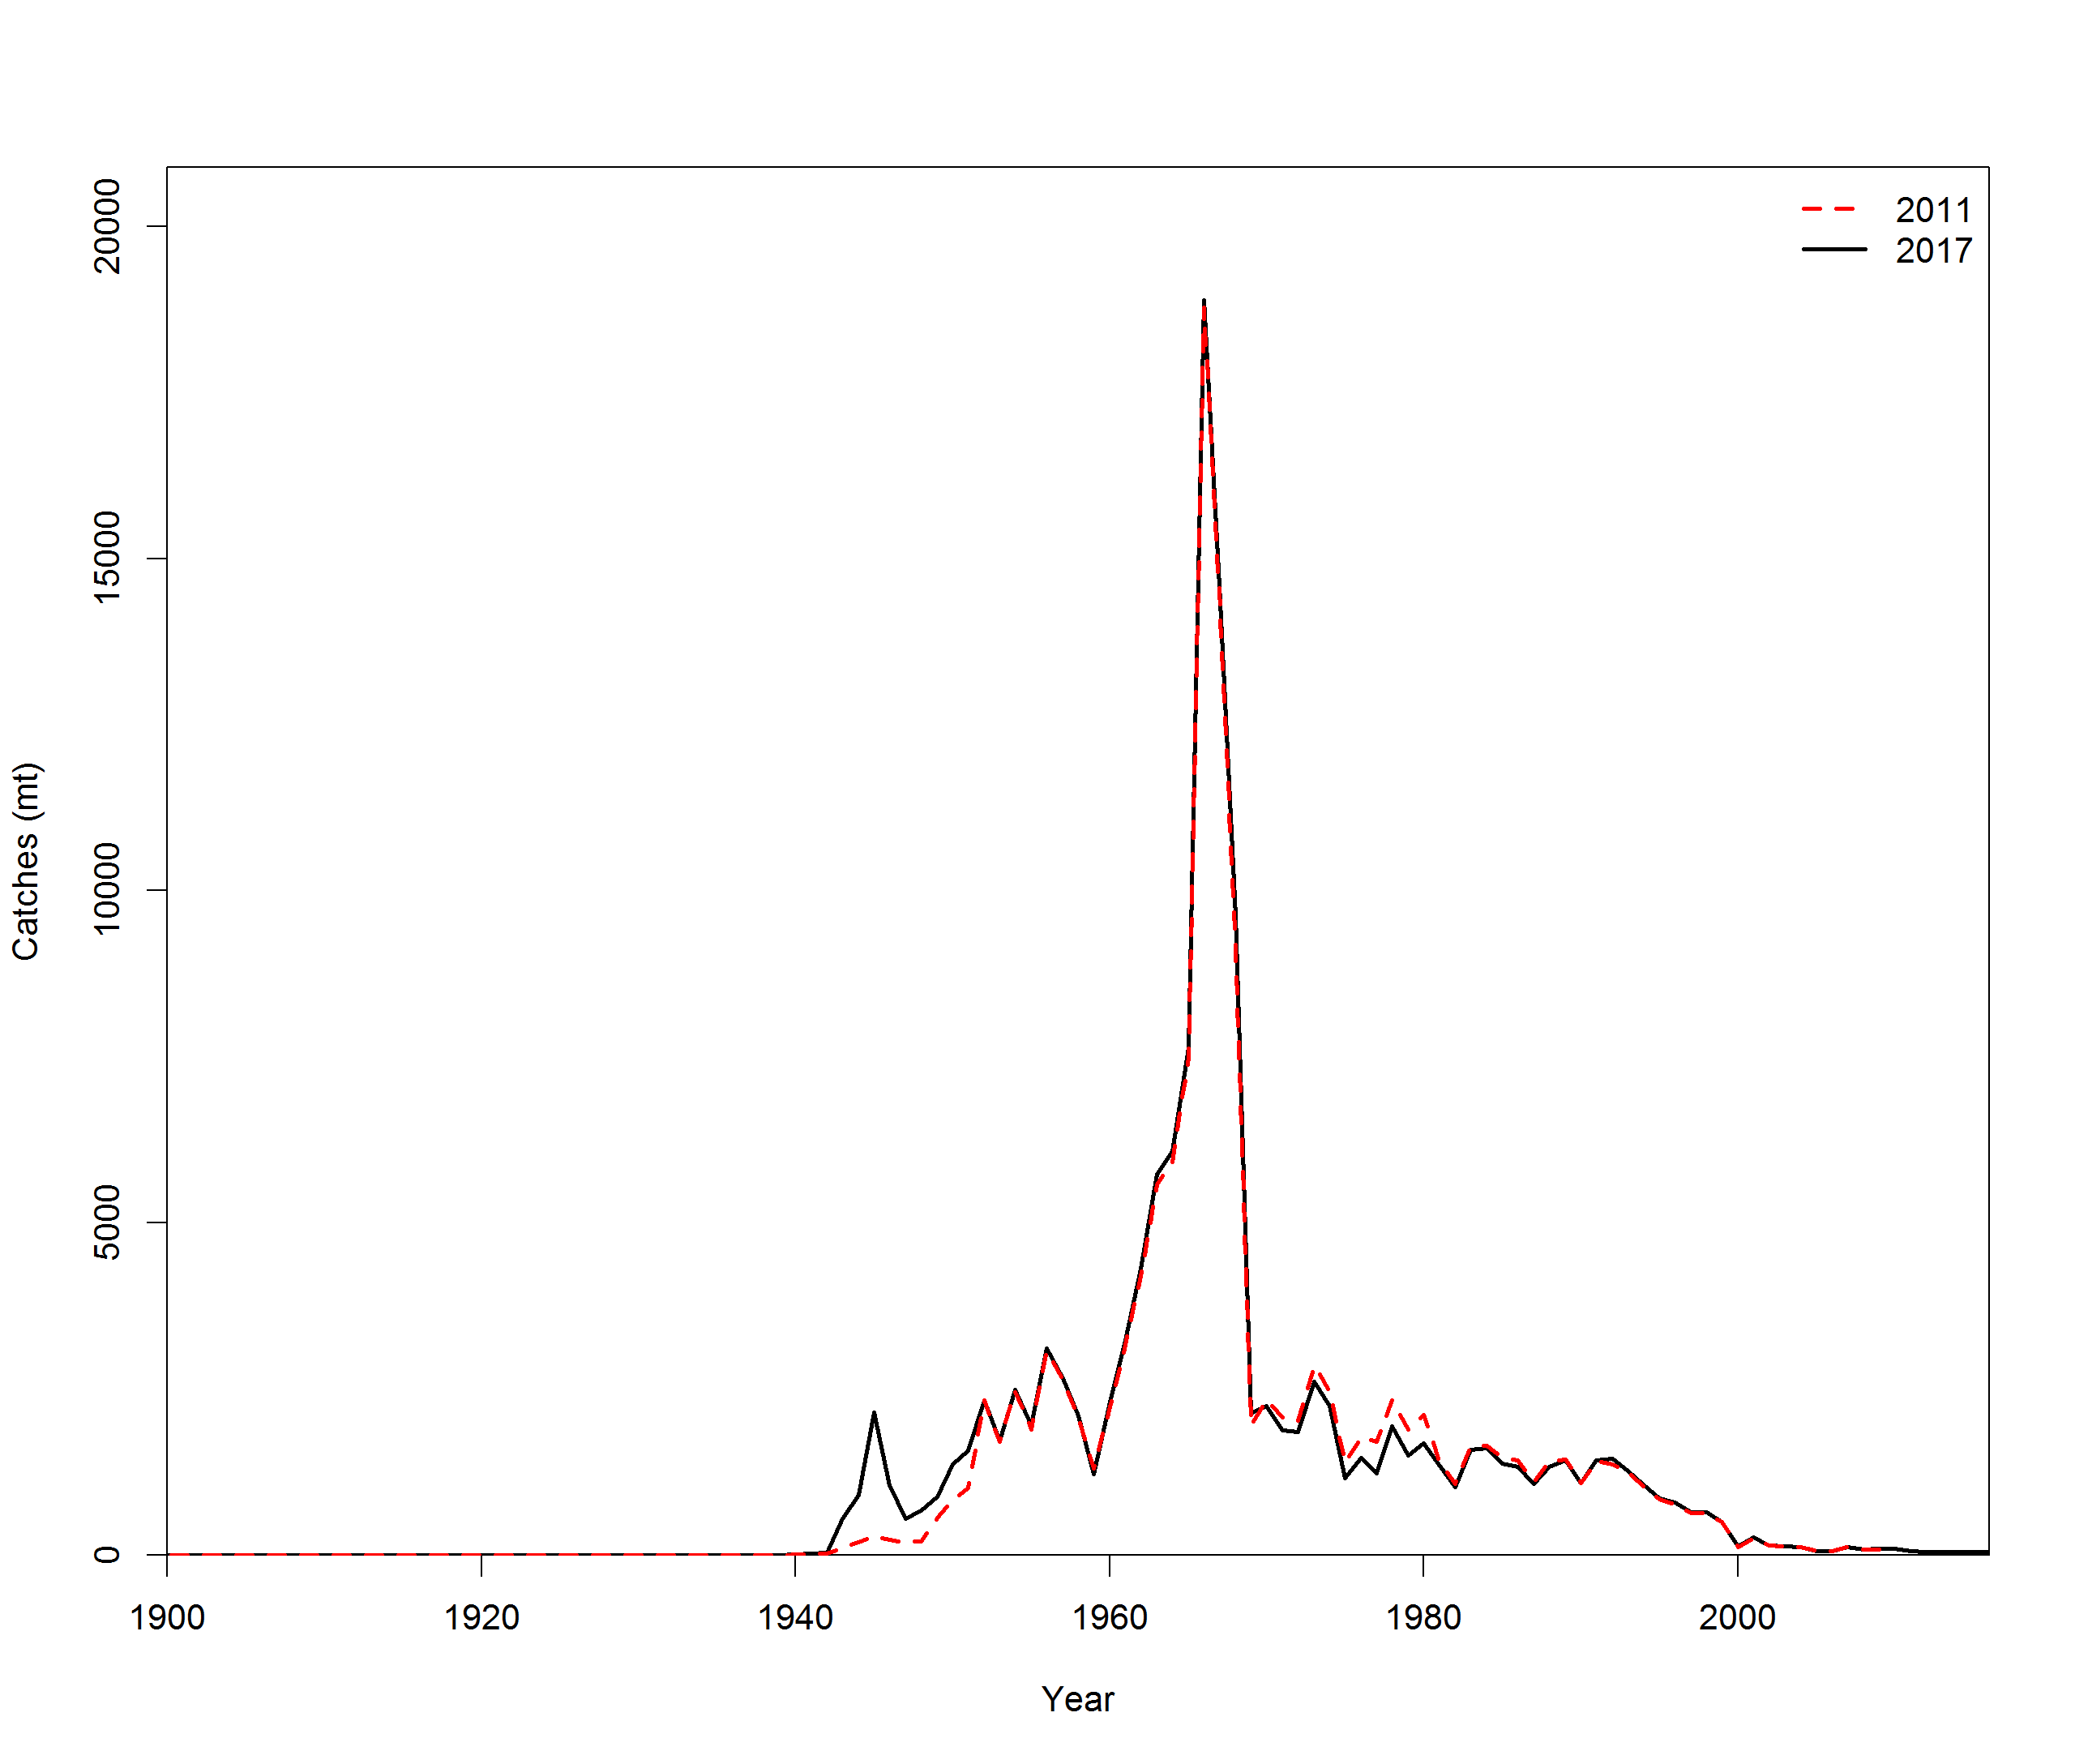
\includegraphics[scale = 0.32, trim={0, 0, 0, 2cm}, clip]{figures/Catch_Comparison.png}
  \end{center}
  *Resulted in $<$ 1\% change in $R0$ 
\end{frame}


\begin{frame}{Landings by Fleet and Survey}
  \begin{center}
    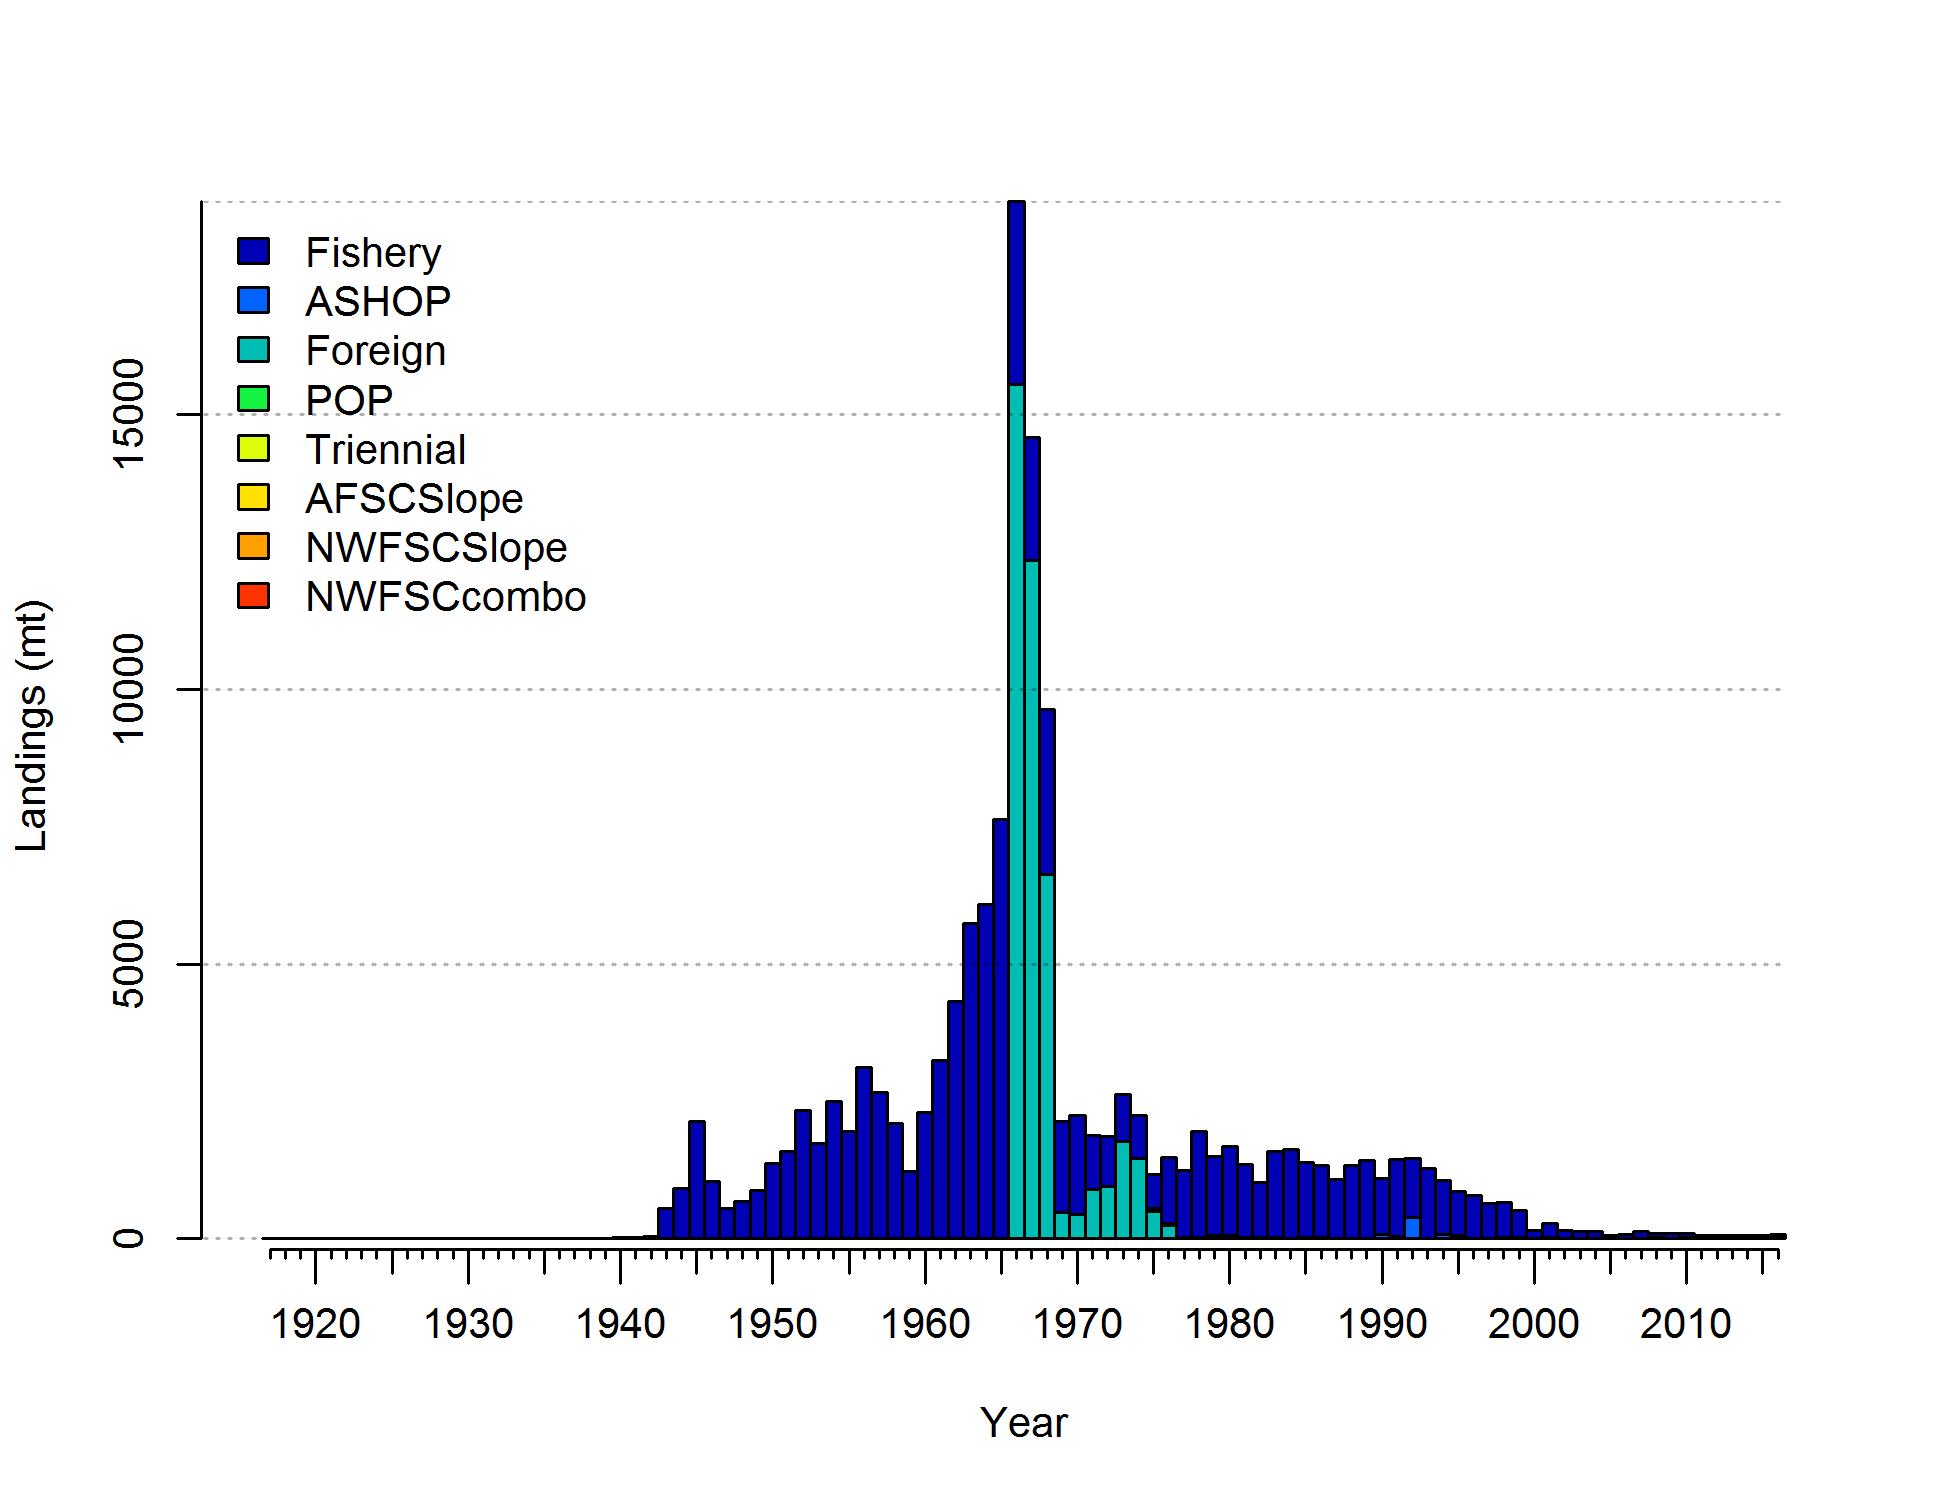
\includegraphics[scale = 0.60]{figures/catch2_landings_stacked.png}
  \end{center}
\end{frame}


\subsection{Discarding practices}
\begin{frame}{Fishery Discard Data}
  \begin{center}
    \includegraphics[scale = 0.40, trim={0, 0, 0, 1cm}, clip]{r4ss/POP_discard_data.png}
  \end{center}
  * \small{Sensitivities done on the 1992 data point (high vs. low) results $\pm$ 0.5\%  in status.}
  \begin{tikzpicture}[remember picture, overlay, shift = {(current page.center)}]
    \node[black] at (-2, -2.15) {\small Pikitch};
    \node[black] at (-0.5,-1.5) {\small Management};
    \node[black] at (-0.5, -1.75) {\small Restrictions};
    \node[black] at (2, 1) {\small WCGOP};
    \draw[black, thick, -] (0.5, 0.8) -- (3, 0.8){};
    \node[black] at (2.5, -2) {\small Post-ITQ};
  \end{tikzpicture}
\end{frame}

%---------------------------------------------------------------------------------
\section{Indices of Abundance}
%---------------------------------------------------------------------------------
\subsection{Fishery CPUE}
\begin{frame}{CPUE}
  \begin{center}
      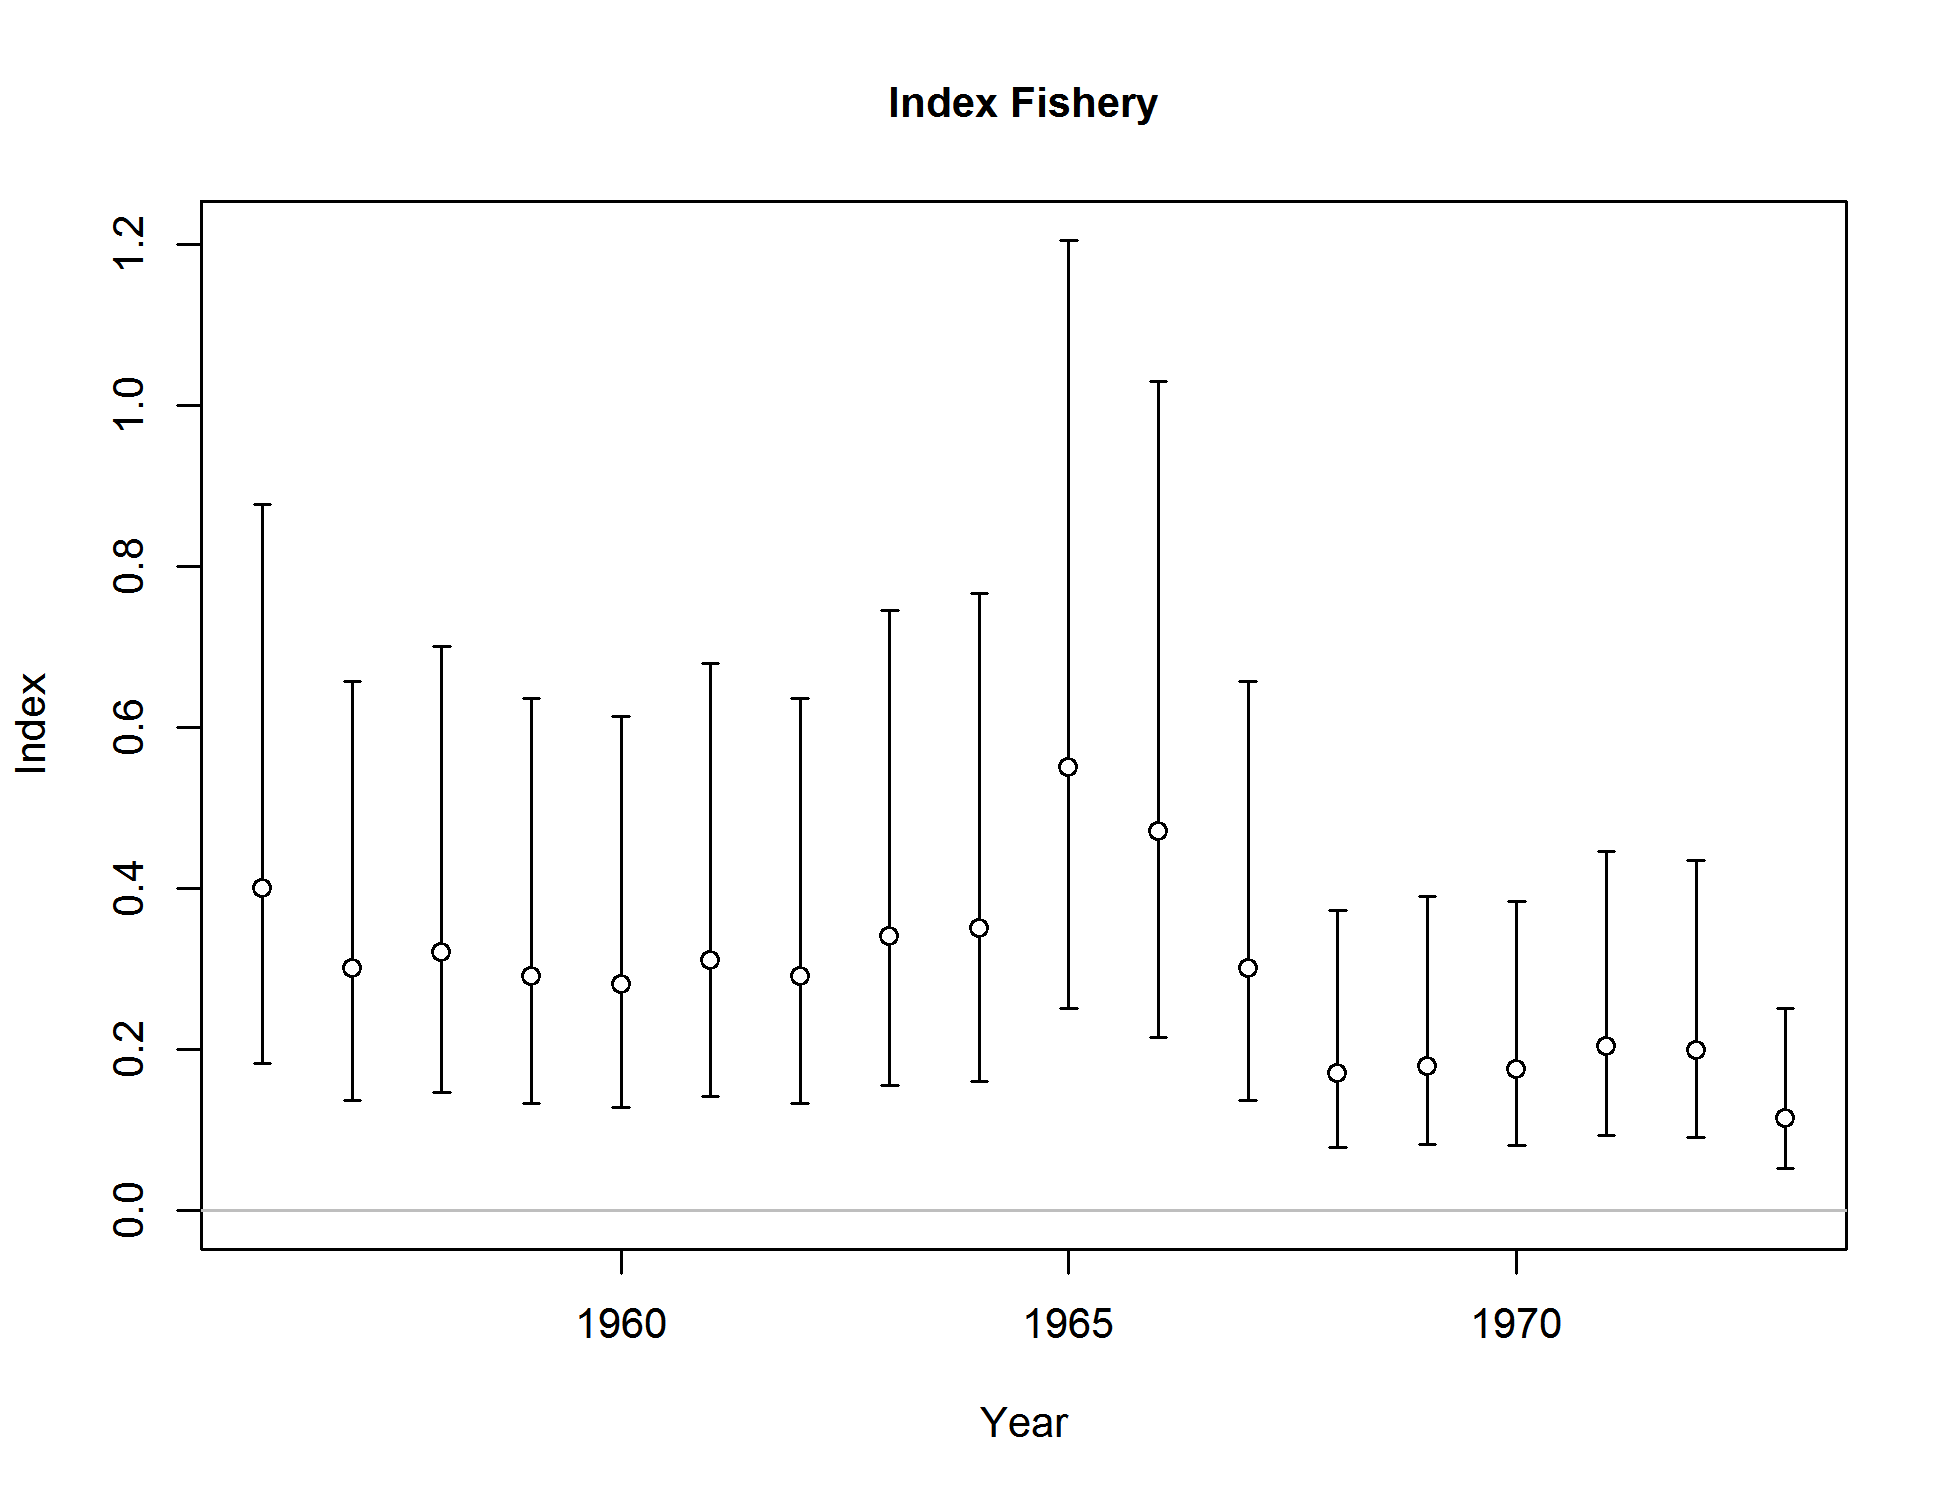
\includegraphics[scale = 0.45]{r4ss/index1_cpuedata_Fishery.png}
  \end{center}
  Gunderson (1977) CPUE from the INPFC Columbia area\\
  *Sensitivity shows little effect on model results when removed.
\end{frame}

\subsection{Survey Indices}
\begin{frame}{Survey Indices}
  \begin{center}
  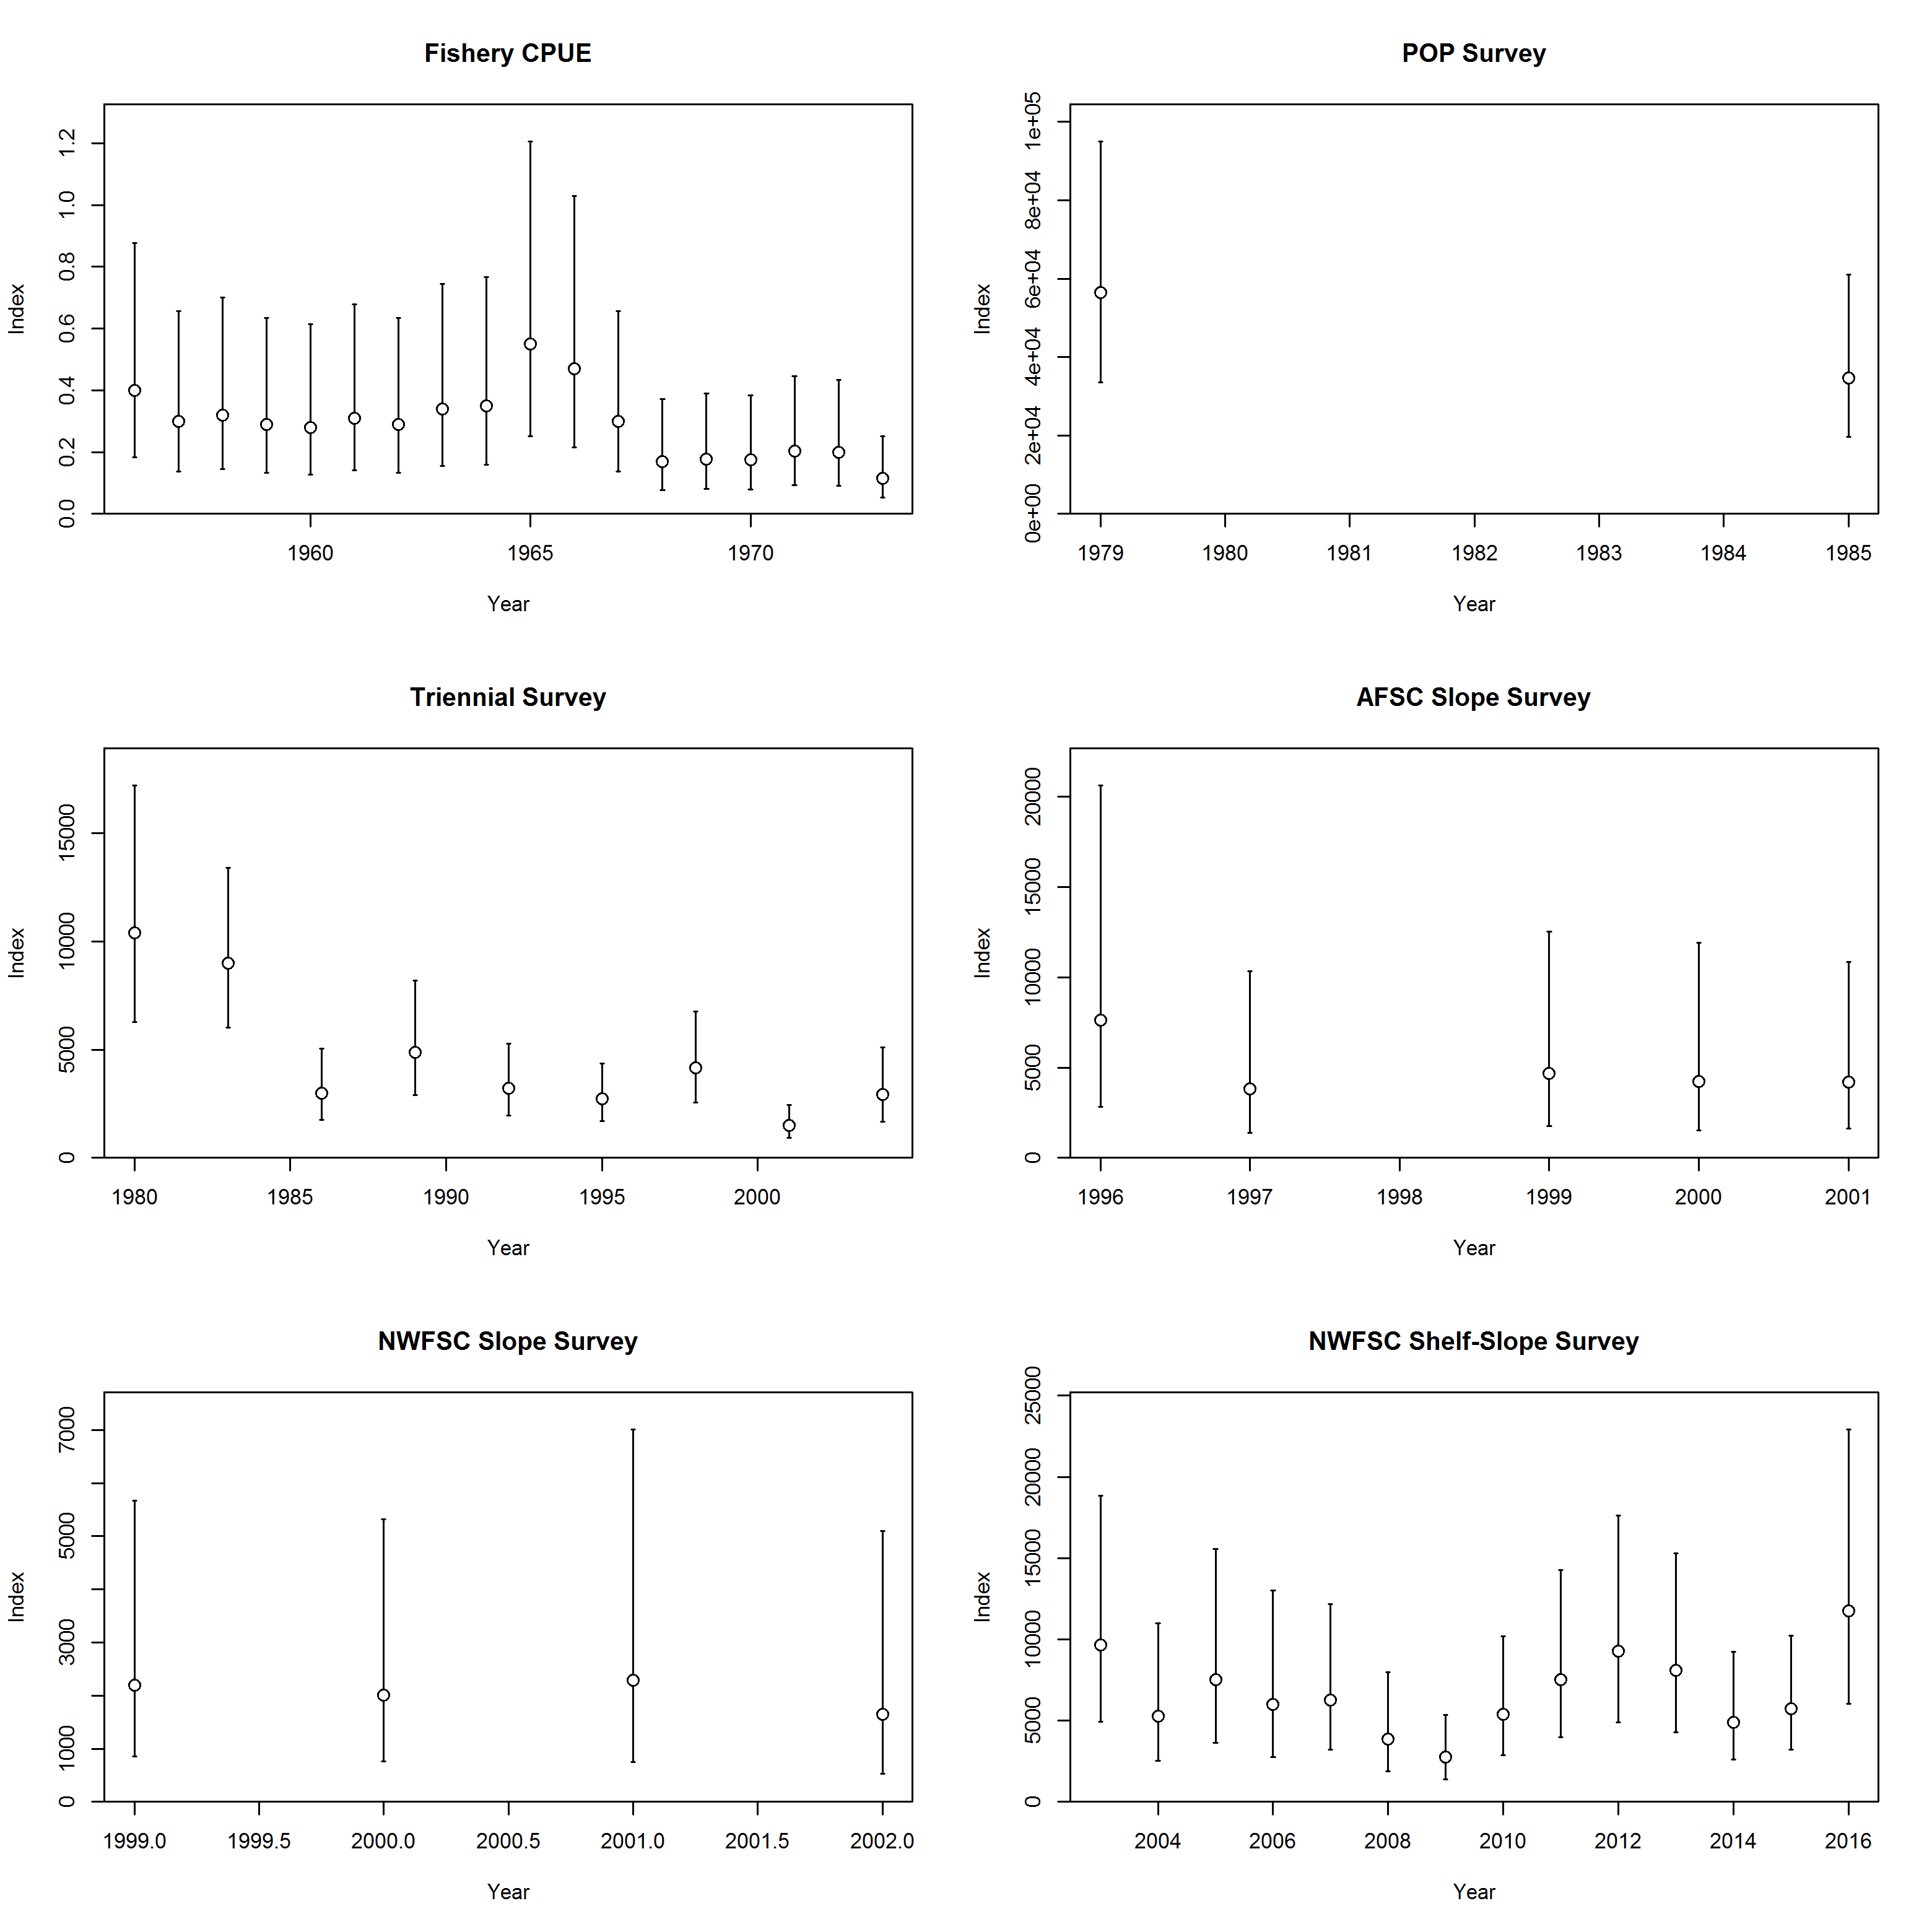
\includegraphics[height = 3in, width = 4in]{figures/Index_Data.png}
  \end{center}
\end{frame}

\begin{frame}{All: Standardized}
  \begin{center}
  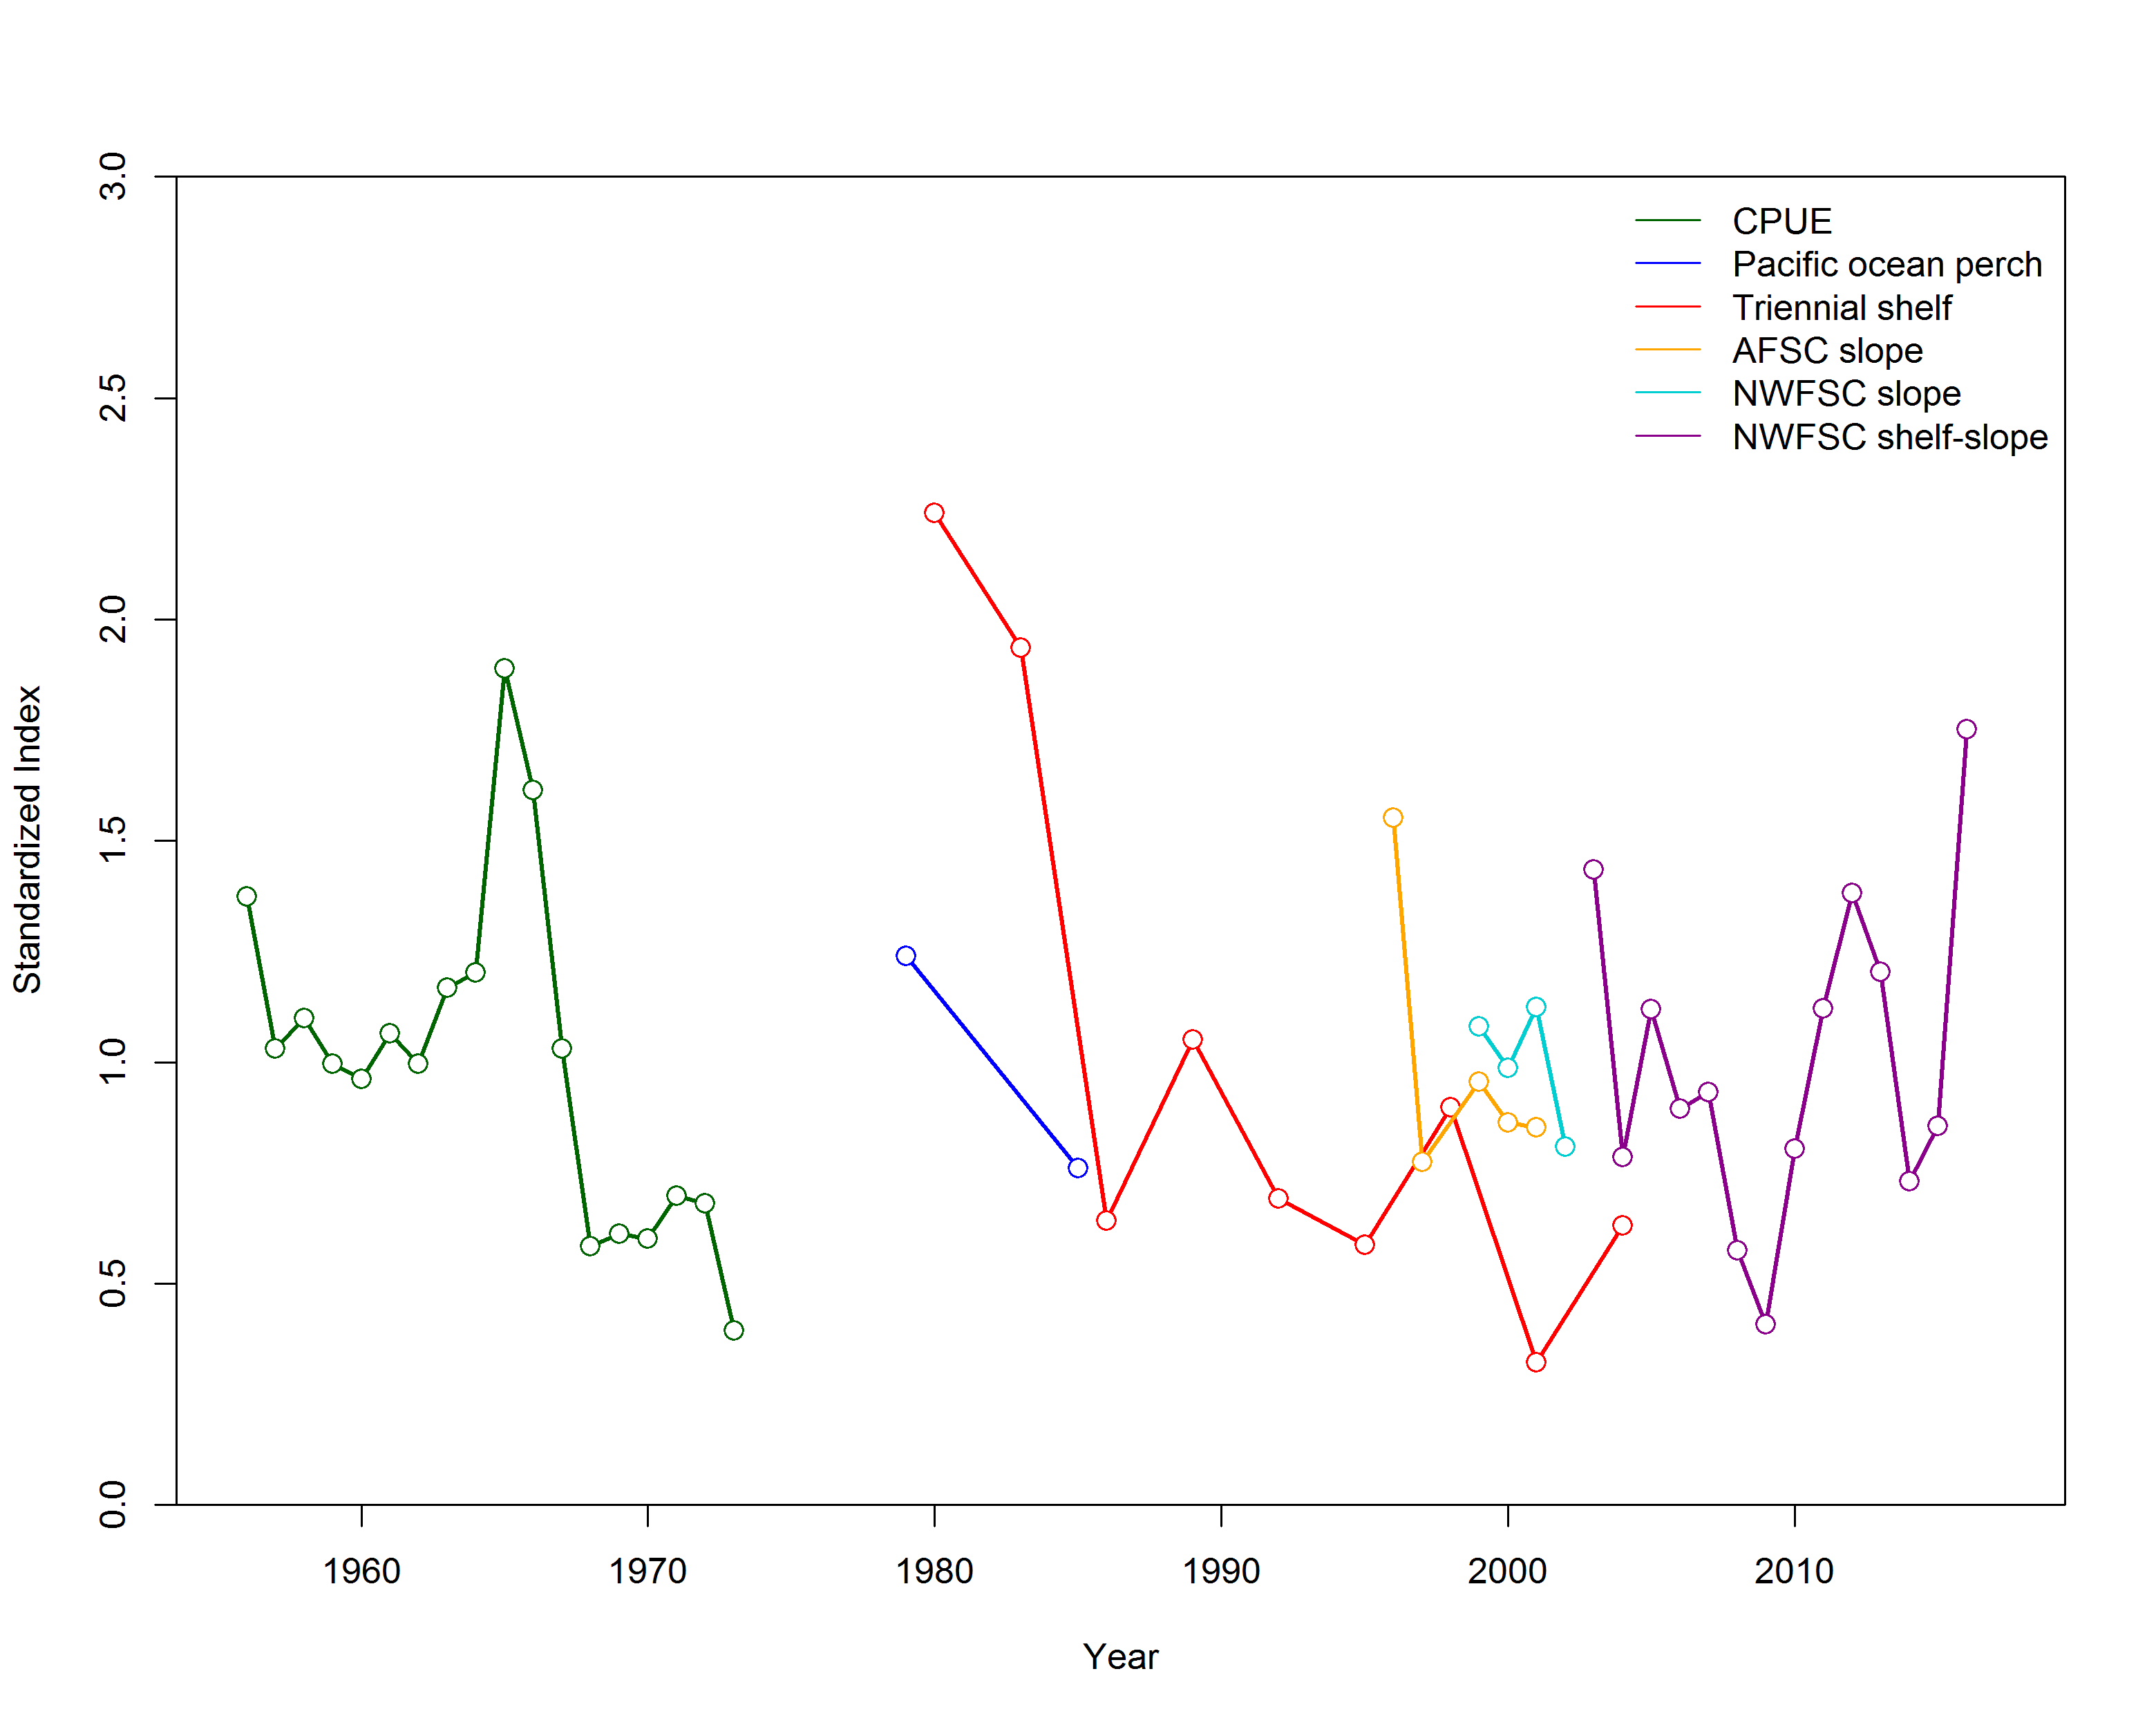
\includegraphics[scale = 0.37]{figures/Index_Standardized.png}
  \end{center}
\end{frame}


%---------------------------------------------------------------------------------
\section{Composition Data}
%---------------------------------------------------------------------------------
\subsection{Fishery Data}
\begin{frame}{Fishery Length and Age Data}
  Fishery length data used in the 2017 assessment:
  \begin{itemize}
    \item Fishery: bottom trawl, mid-water trawl, fixed gear
      \begin{itemize}
        \item Retained Lengths: 1966-2016
        \item Discarded Lengths: 1986 (Pikitch), 2004-2015
        \item Ages: 1981-1988, 1994, 1999-2016
      \end{itemize}
    \item At-sea hake fishery
      \begin{itemize}
        \item All (Retained and Discarded) Lengths: 2003-2016
        \item Ages: 2003, 2006, 2007, 2014
      \end{itemize}
  \end{itemize}
\end{frame}

\begin{frame}{Fishery Lengths: Discarded}
   \begin{center}
   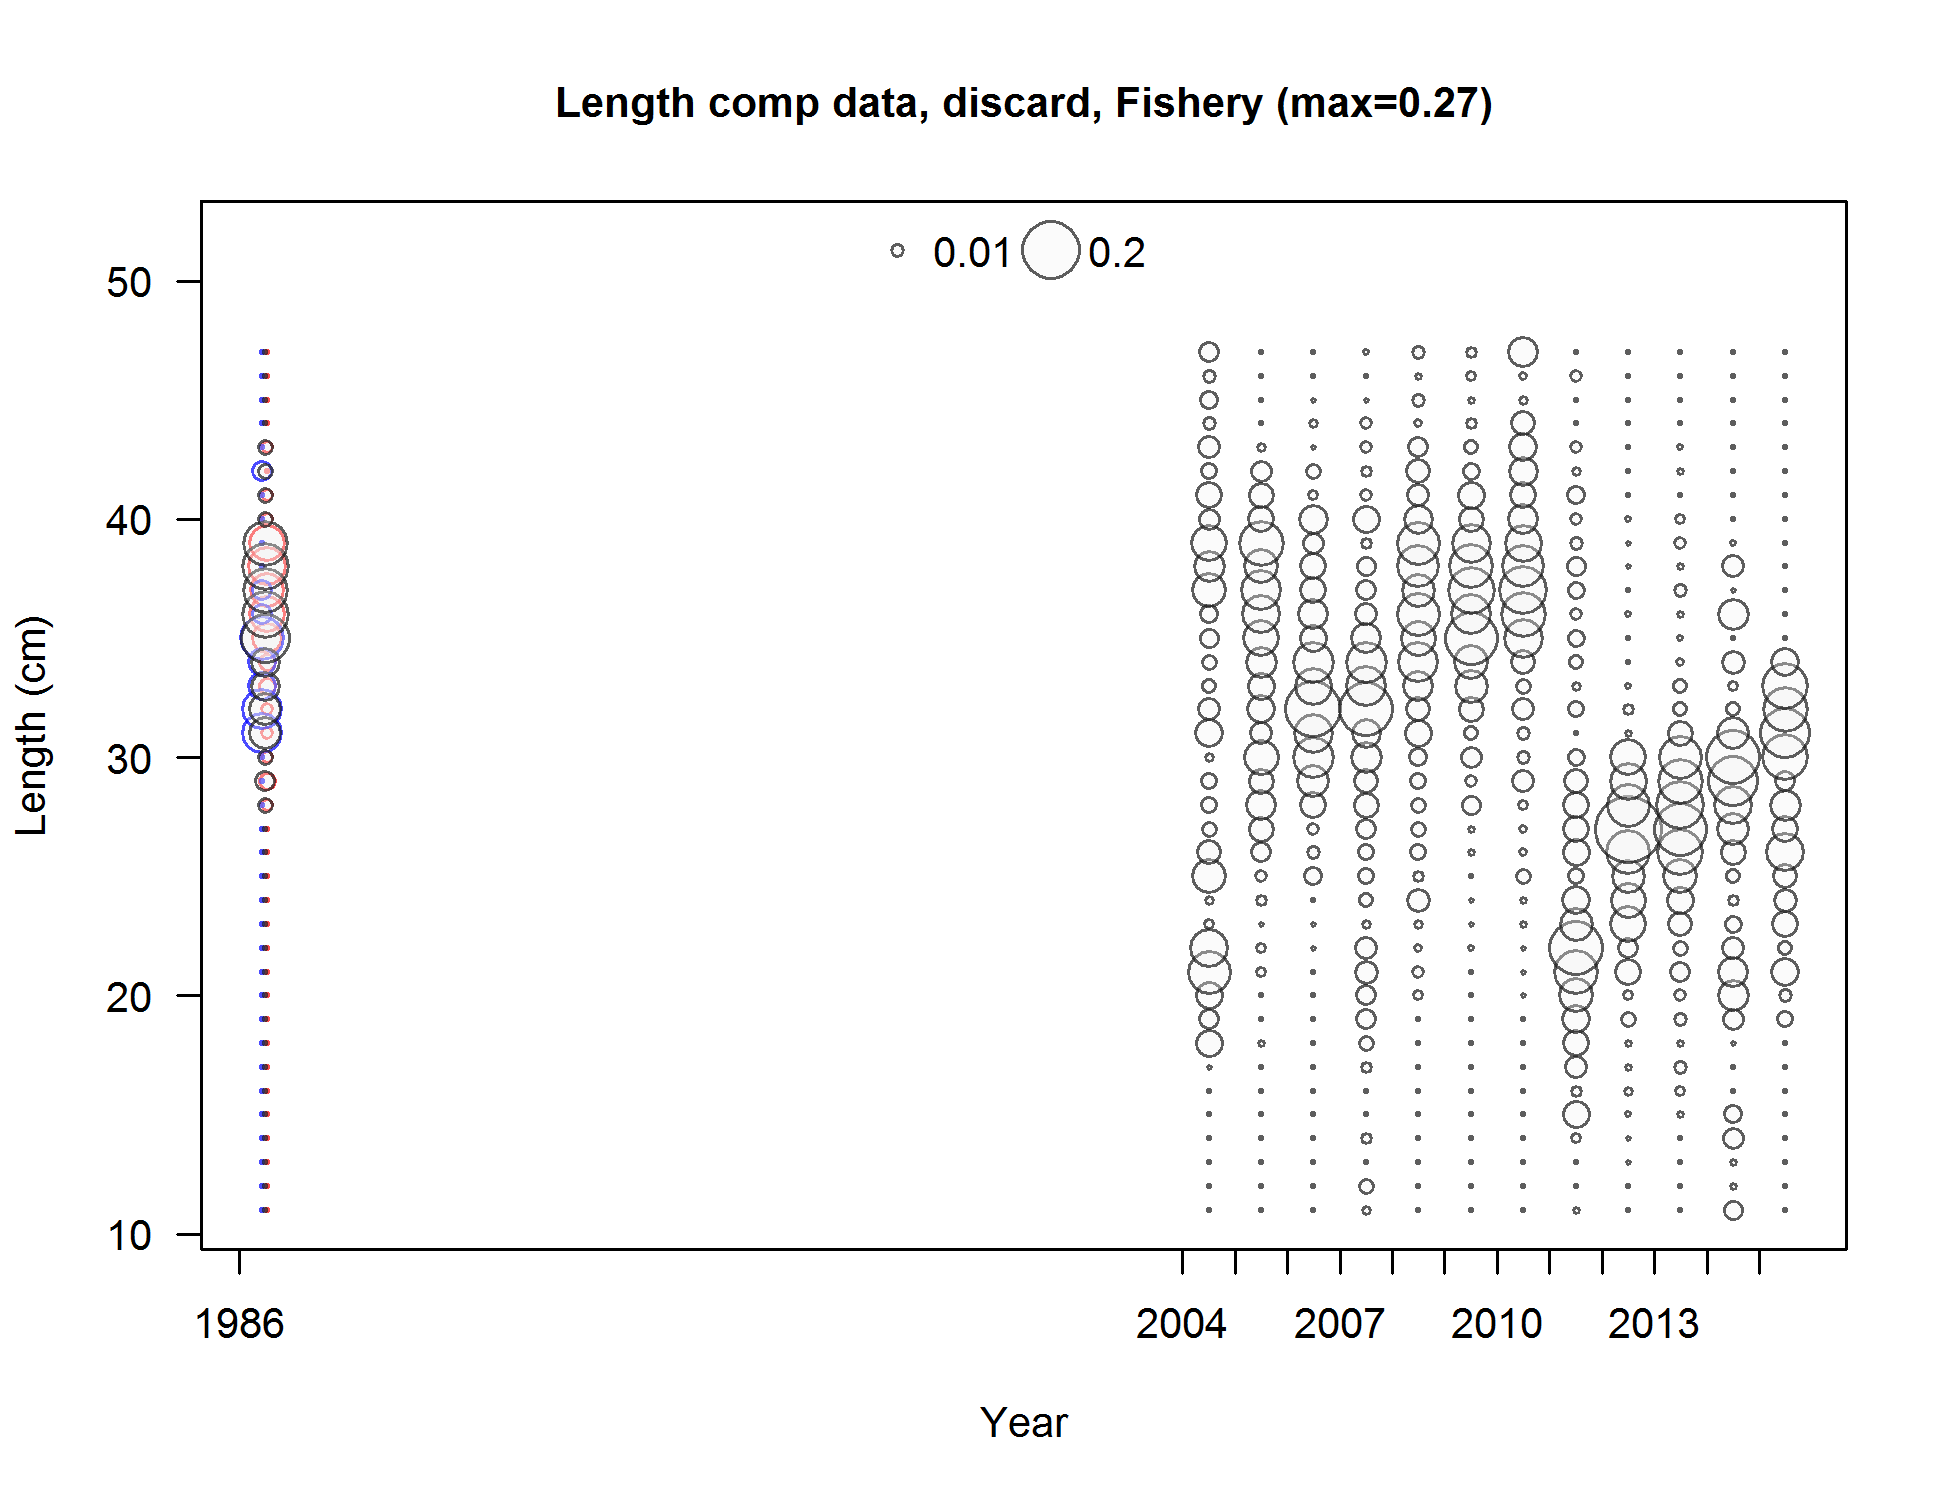
\includegraphics[scale = 0.50]{r4ss/comp_lendat_bubflt1mkt1.png}
   \end{center}
\end{frame}

\begin{frame}{Fishery Lengths and Ages: Retained}
   \includegraphics[scale = 0.37]{r4ss/comp_lendat_bubflt1mkt2_page4.png}
   \includegraphics[scale = 0.37]{r4ss/comp_agedat_bubflt1mkt2_page2.png}
\end{frame}


\begin{frame}{At-sea hake}
  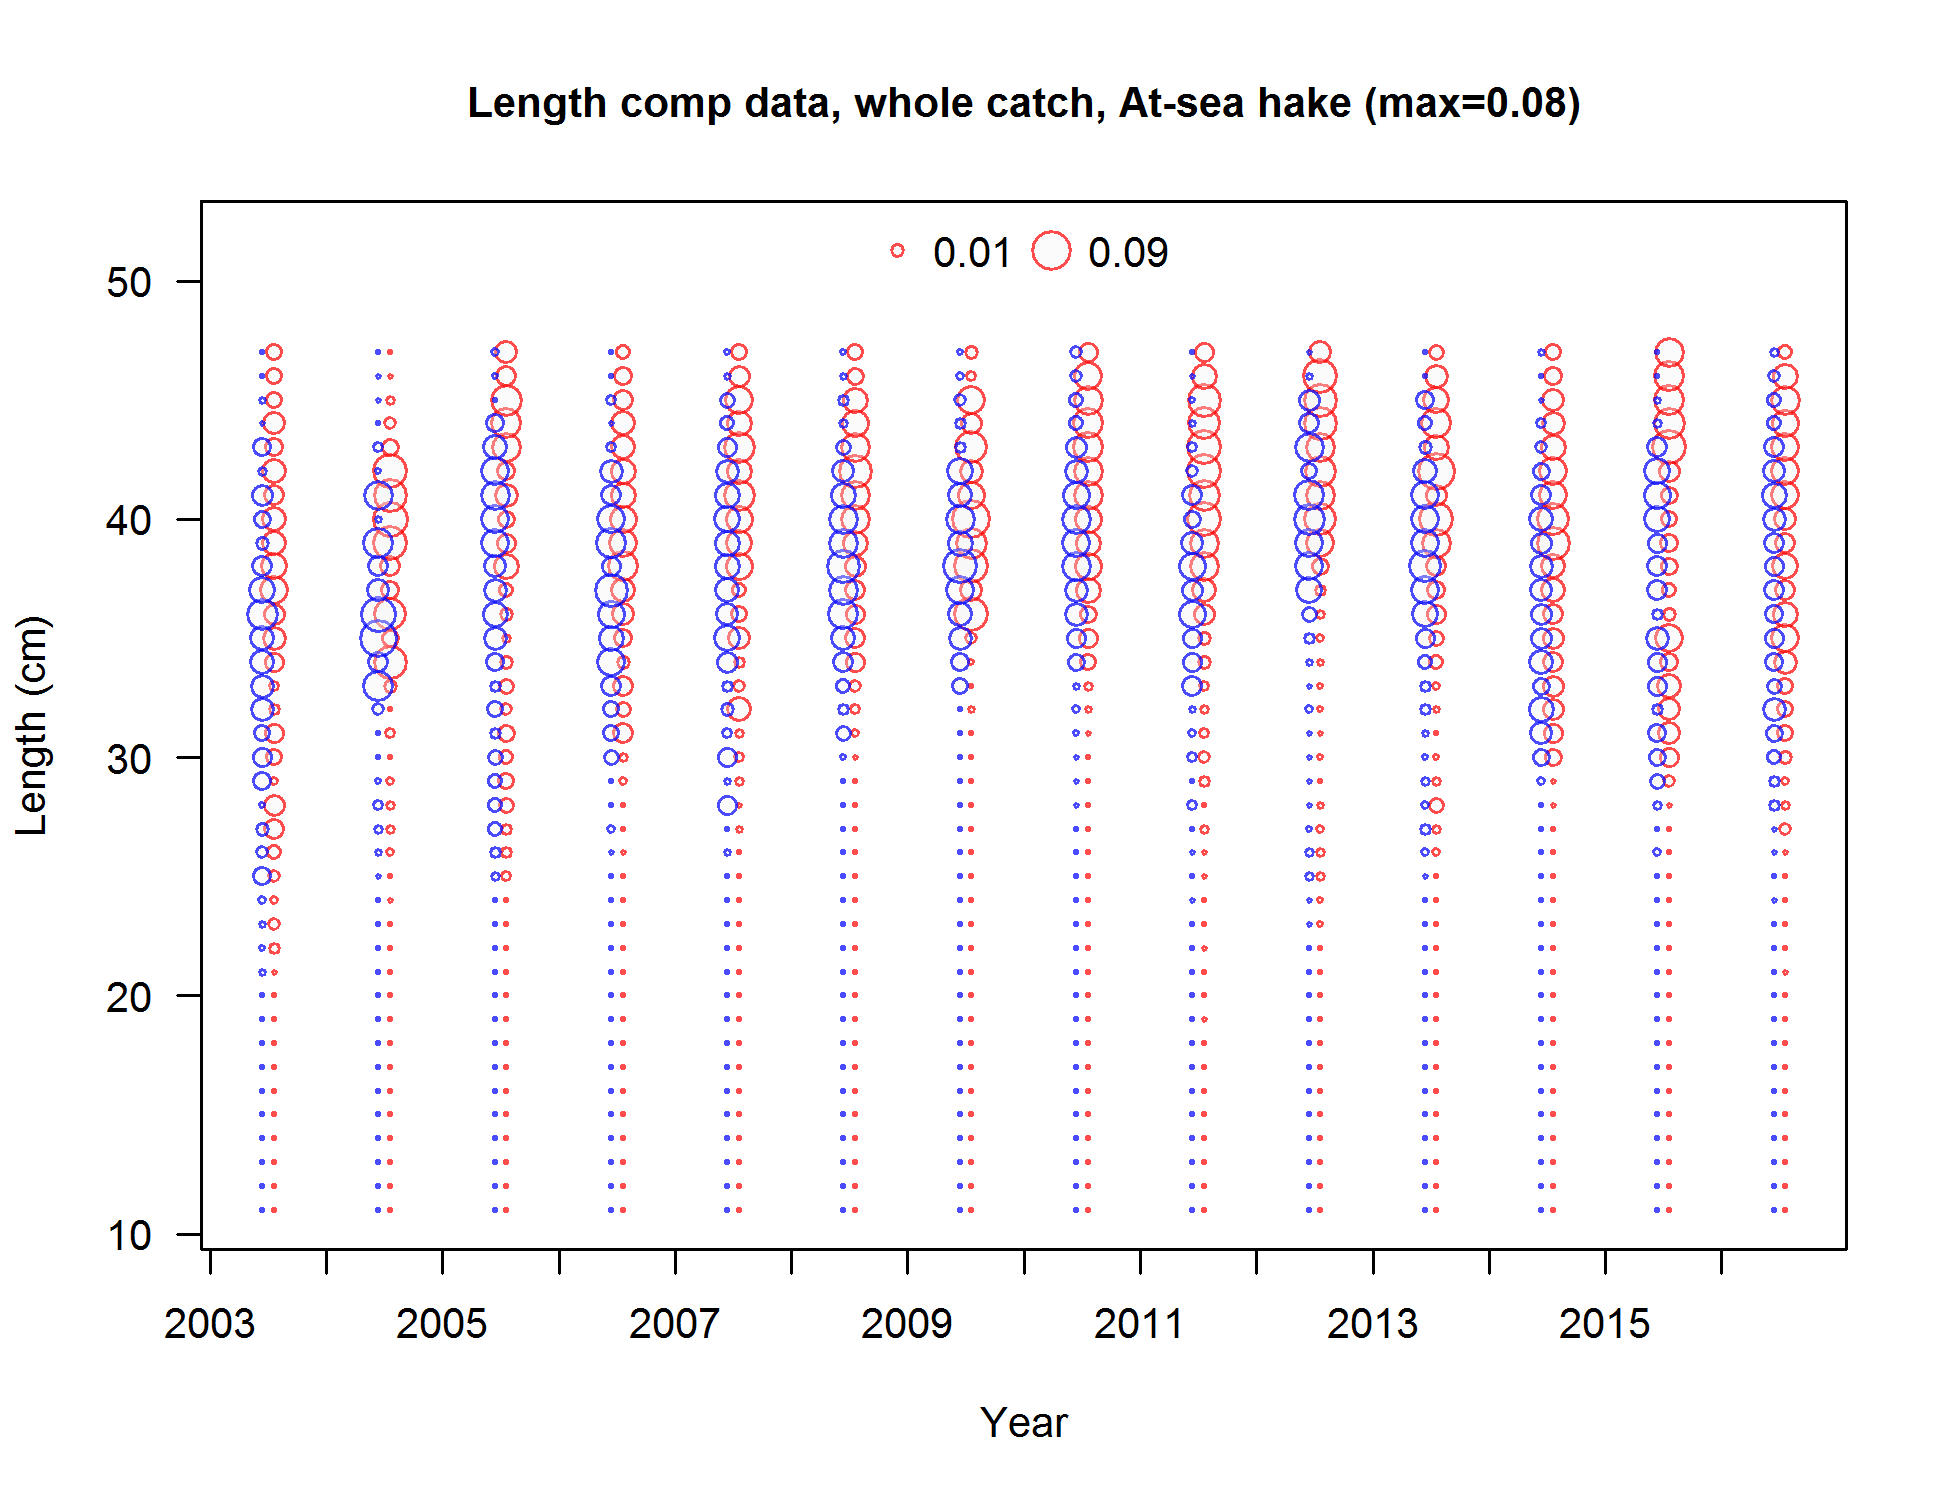
\includegraphics[scale = 0.37]{r4ss/comp_lendat_bubflt2mkt0.png}
  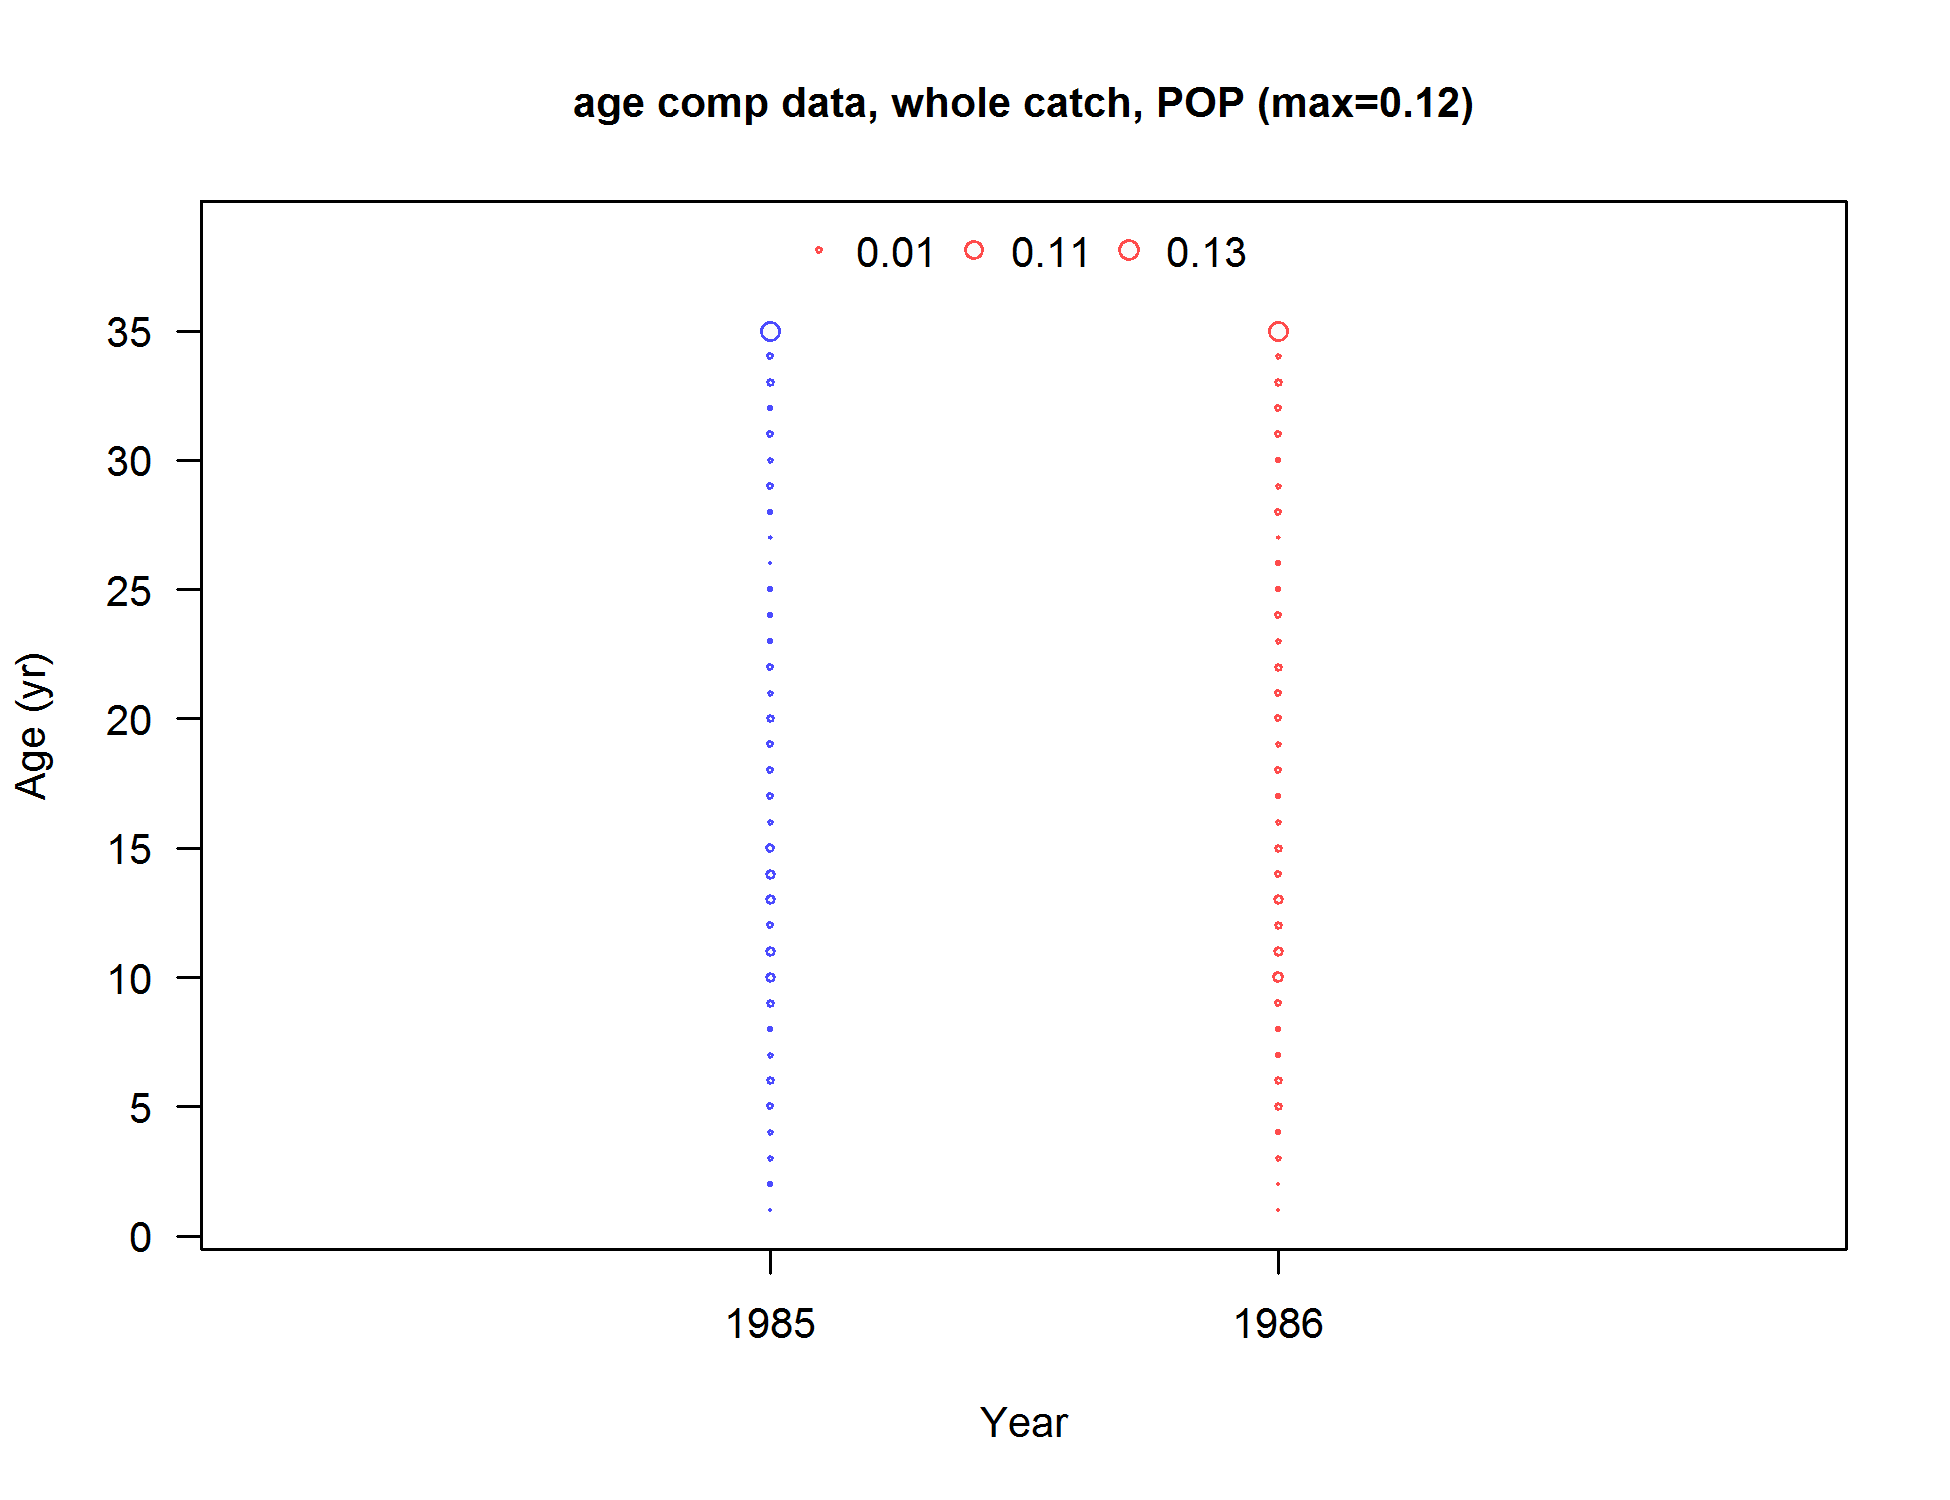
\includegraphics[scale = 0.37]{r4ss/comp_agedat_bubflt2mkt0.png}
\end{frame}

\subsection{Survey Length and Age Data}
\begin{frame}{Survey Length Data}
  Survey length data used in the 2017 assessment:
  \begin{itemize}
    \item Pacific ocean perch survey
      \begin{itemize}
        \item Lengths: 1979 and 1985
        \item Ages: 1985
      \end{itemize}
    \item Triennial shelf survey
      \begin{itemize}
        \item Lengths: 1980, 1983, 1986, 1989, 1992, 1995, 1998, 2001, 2004
        \item Ages: 1989, 1992, 1995, 1998, 2001, 2004
      \end{itemize}
    \item AFSC slope survey
      \begin{itemize}
        \item Lengths: 1996, 1997, 1999-2001
      \end{itemize}
    \item NWFSC slope survey
      \begin{itemize}
        \item Lengths: 2001 and 2002
        \item Ages: 2001 and 2002
      \end{itemize}
    \item NWFSC shelf-slope survey
      \begin{itemize}
        \item Lengths: 2003-2016
        \item Ages: 2003-2016
      \end{itemize}
  \end{itemize}
\end{frame}


\begin{frame}{Pacific ocean perch survey lengths}
  \includegraphics[scale = 0.37]{r4ss/comp_lendat_bubflt4mkt0.png}
  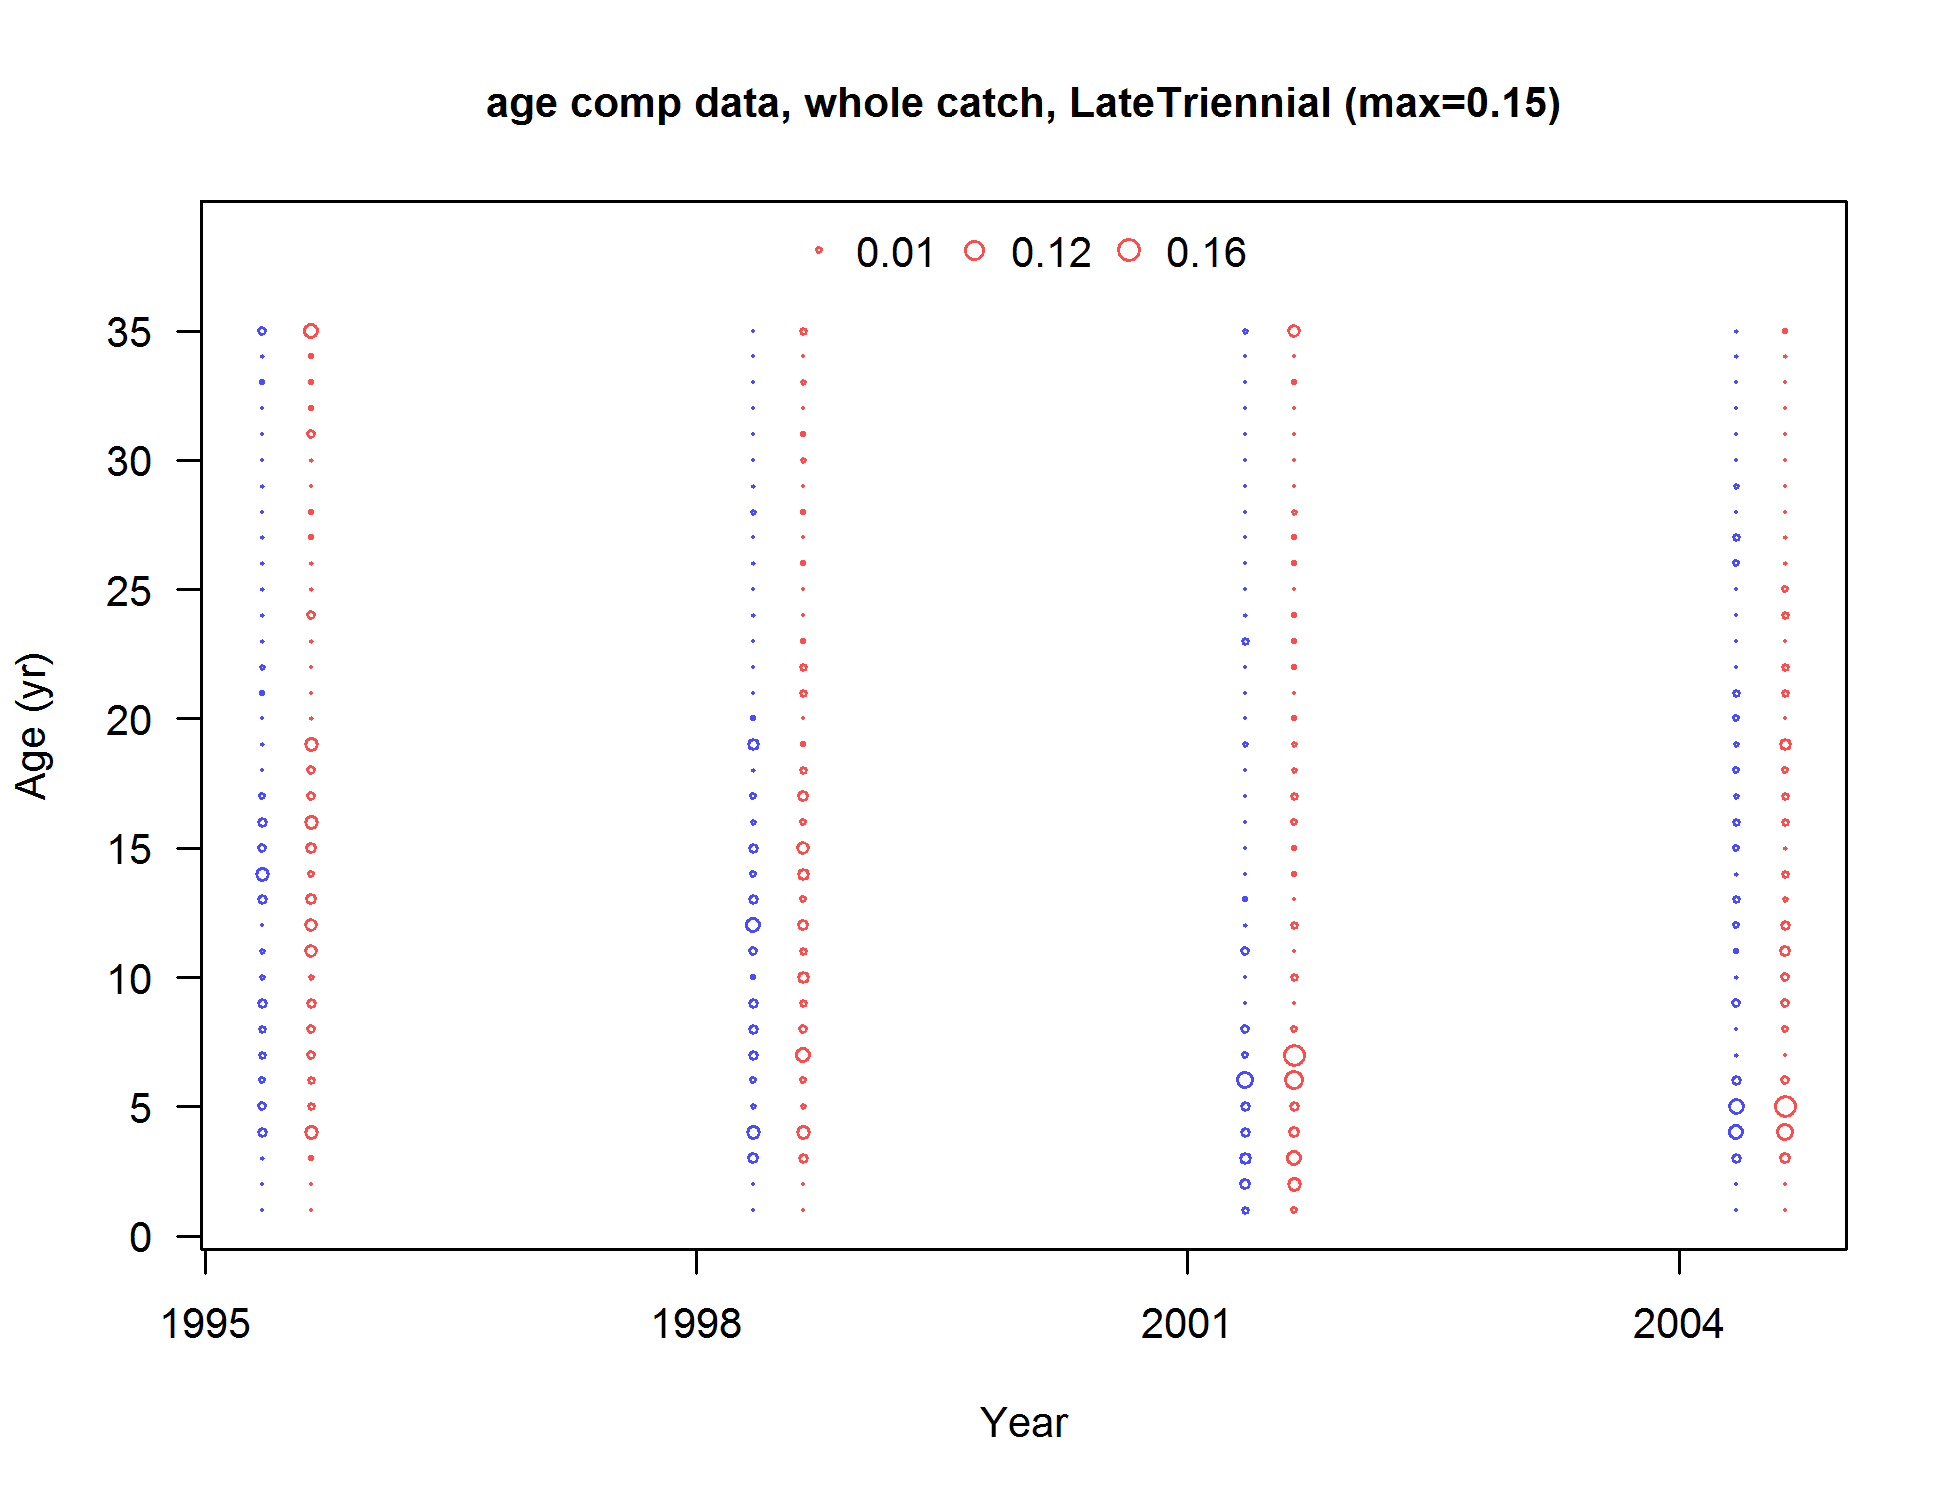
\includegraphics[scale = 0.37]{r4ss/comp_agedat_bubflt4mkt0.png}
\end{frame}

\begin{frame}{Triennial shelf survey }
  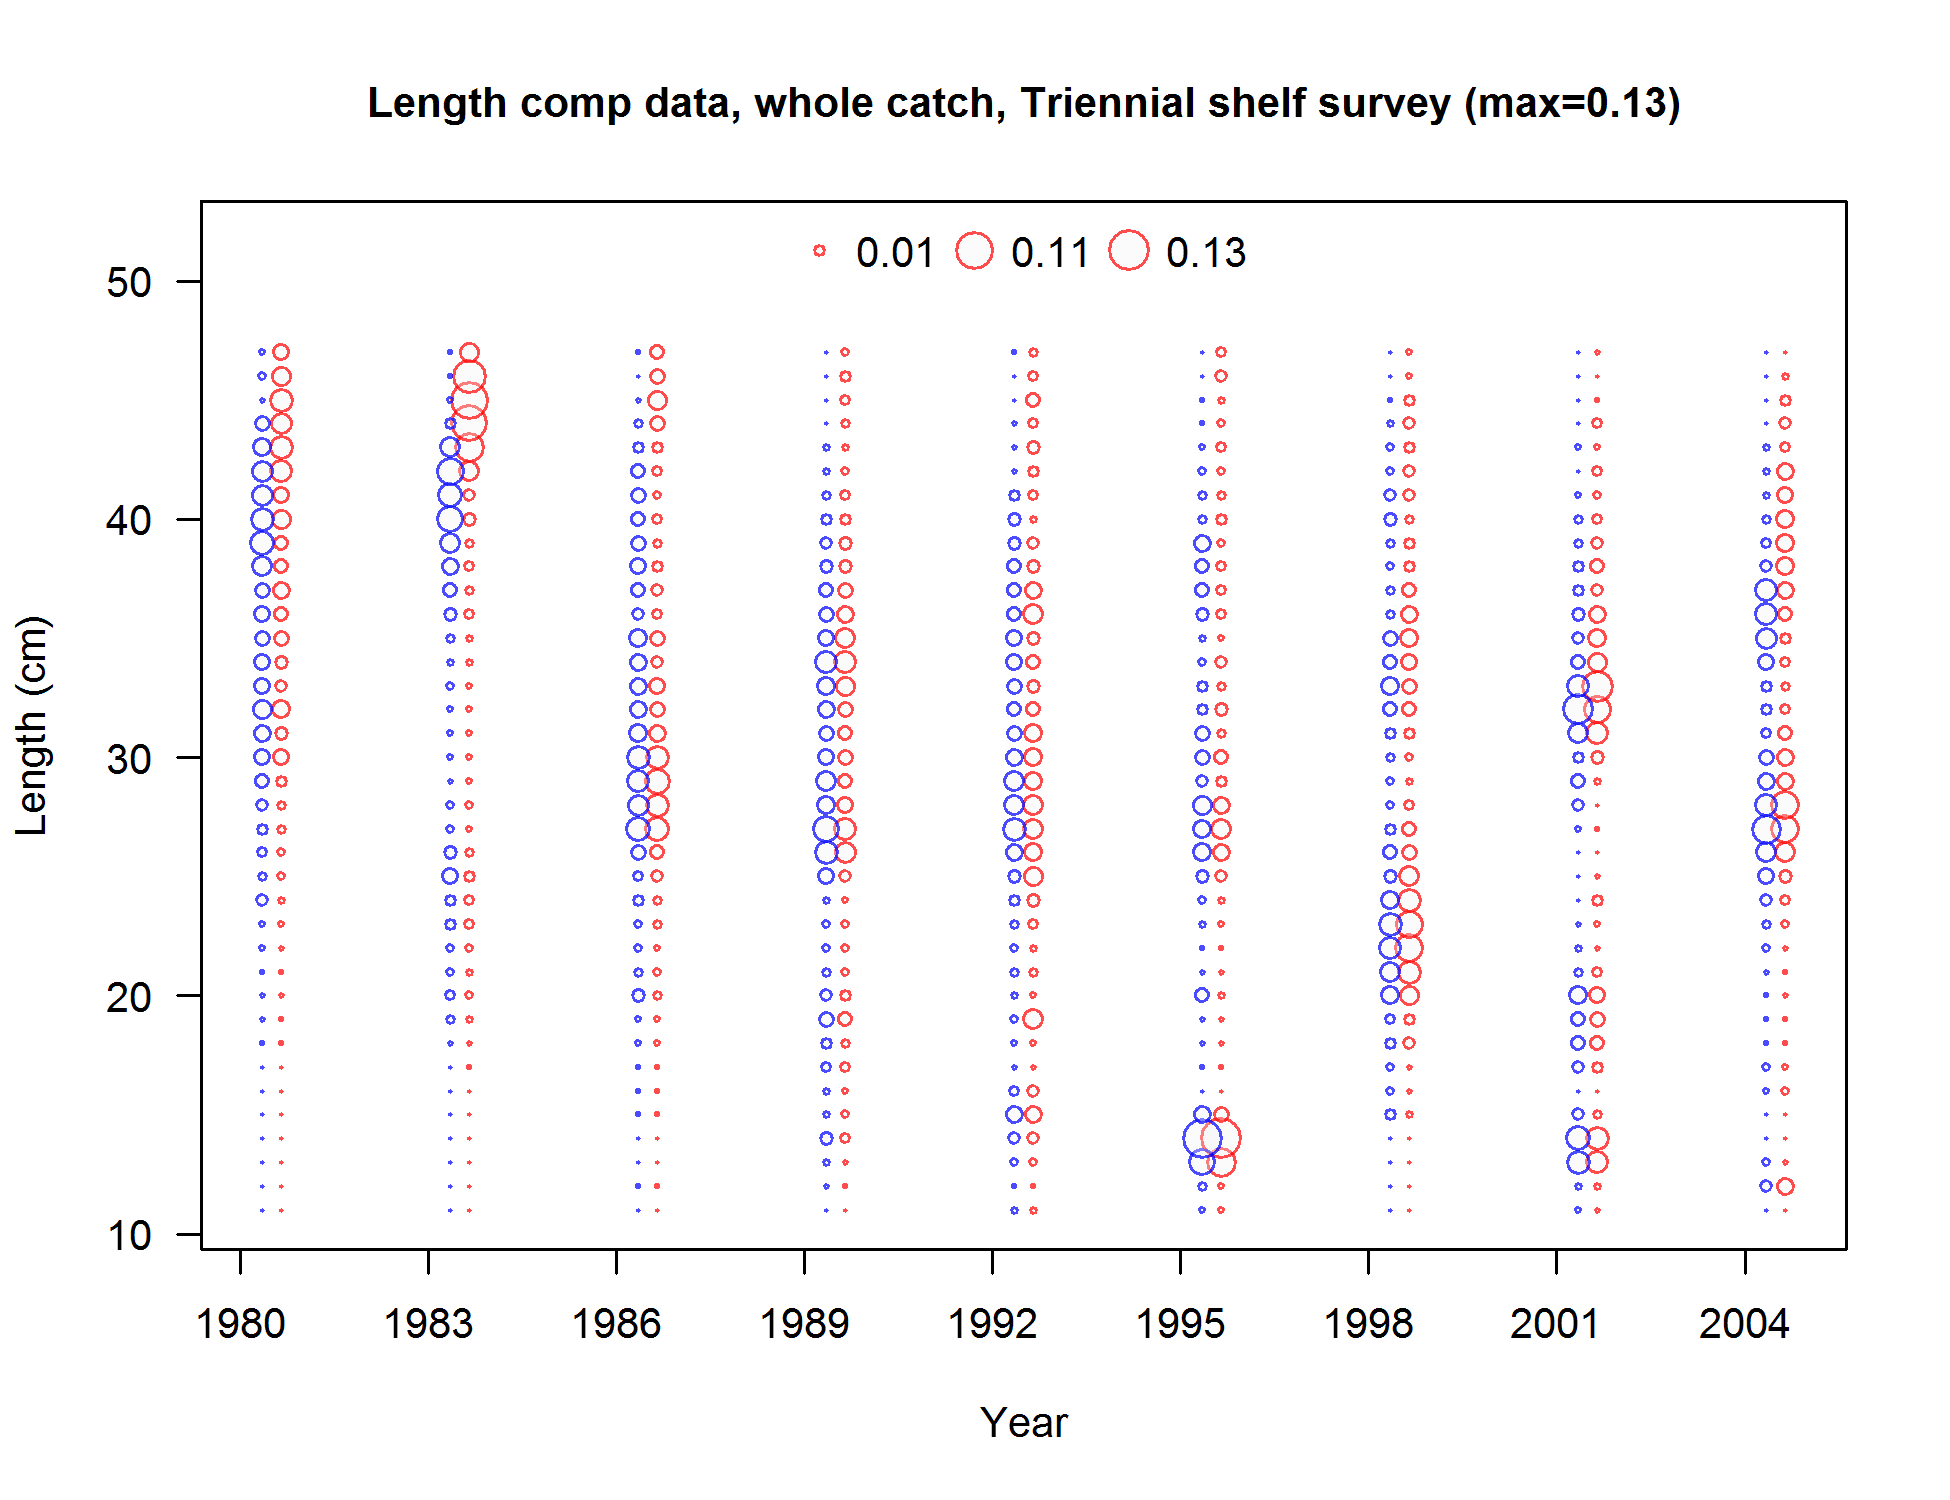
\includegraphics[scale = 0.37]{r4ss/comp_lendat_bubflt5mkt0.png}
  \includegraphics[scale = 0.37]{r4ss/comp_agedat_bubflt5mkt0.png}
\end{frame}

\begin{frame}{AFSC slope survey }
  \includegraphics[scale = 0.37]{r4ss/comp_lendat_bubflt6mkt0.png}
  
\end{frame}

\begin{frame}{NWFSC slope survey }
    \includegraphics[scale = 0.37]{r4ss/comp_lendat_bubflt7mkt0.png}
    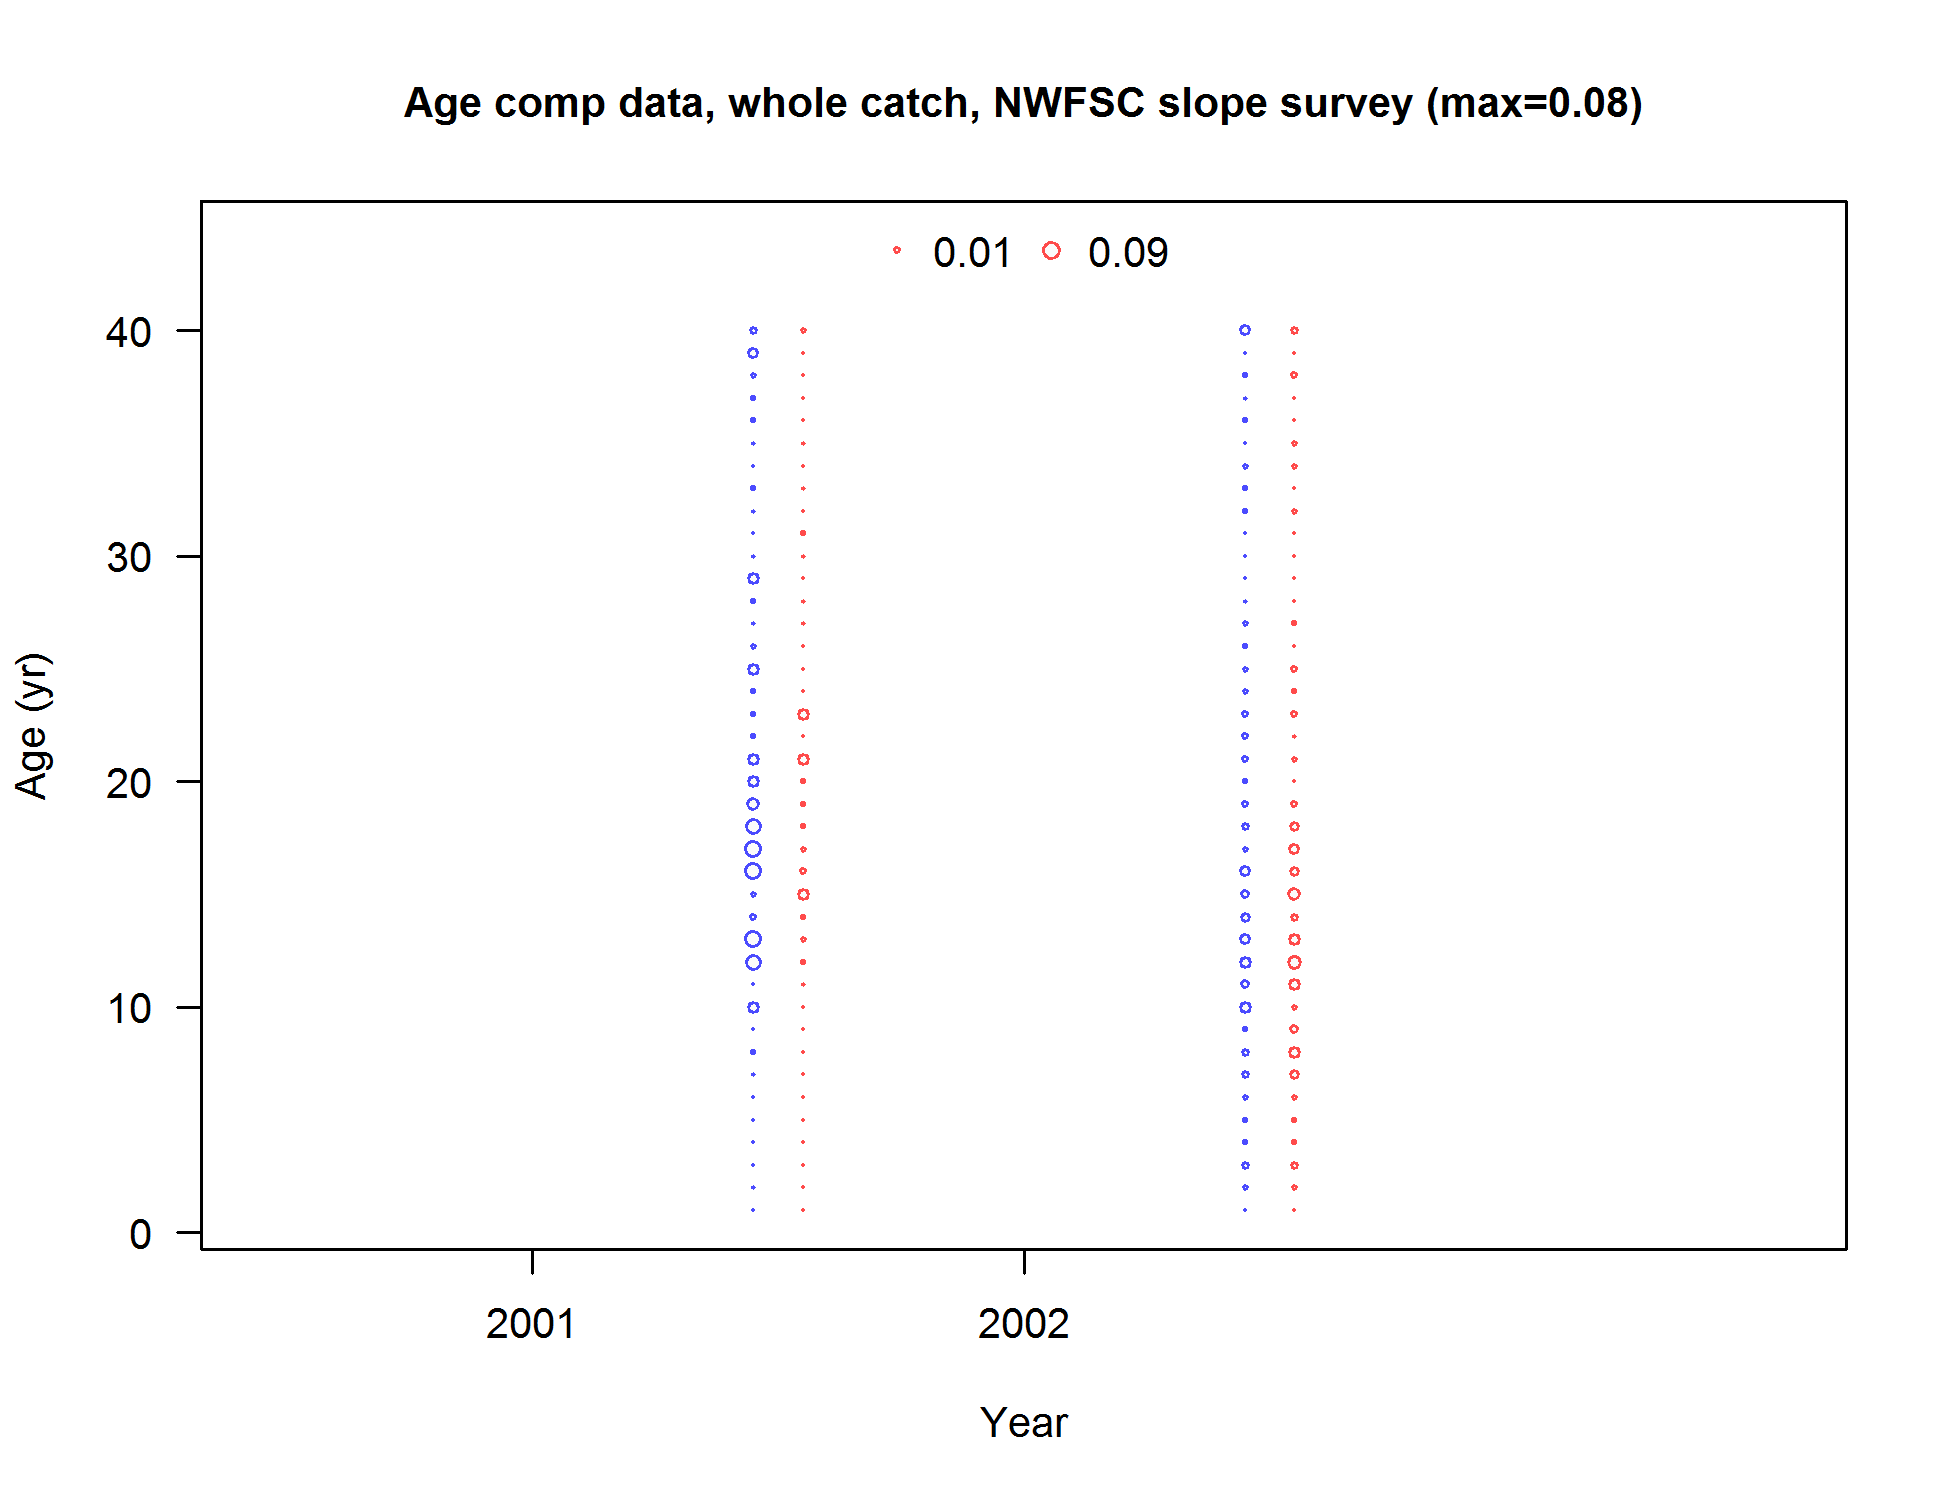
\includegraphics[scale = 0.37]{r4ss/comp_agedat_bubflt7mkt0.png}

\end{frame}

\begin{frame}{NWFSC shelf-slope survey }
  \includegraphics[scale = 0.37]{r4ss/comp_lendat_bubflt8mkt0.png}
  \includegraphics[scale = 0.37]{r4ss/comp_gstagedat_bubflt8mkt0.png}
\end{frame}


\begin{frame}{NWFSC shelf-slope conditional age-at-length}
    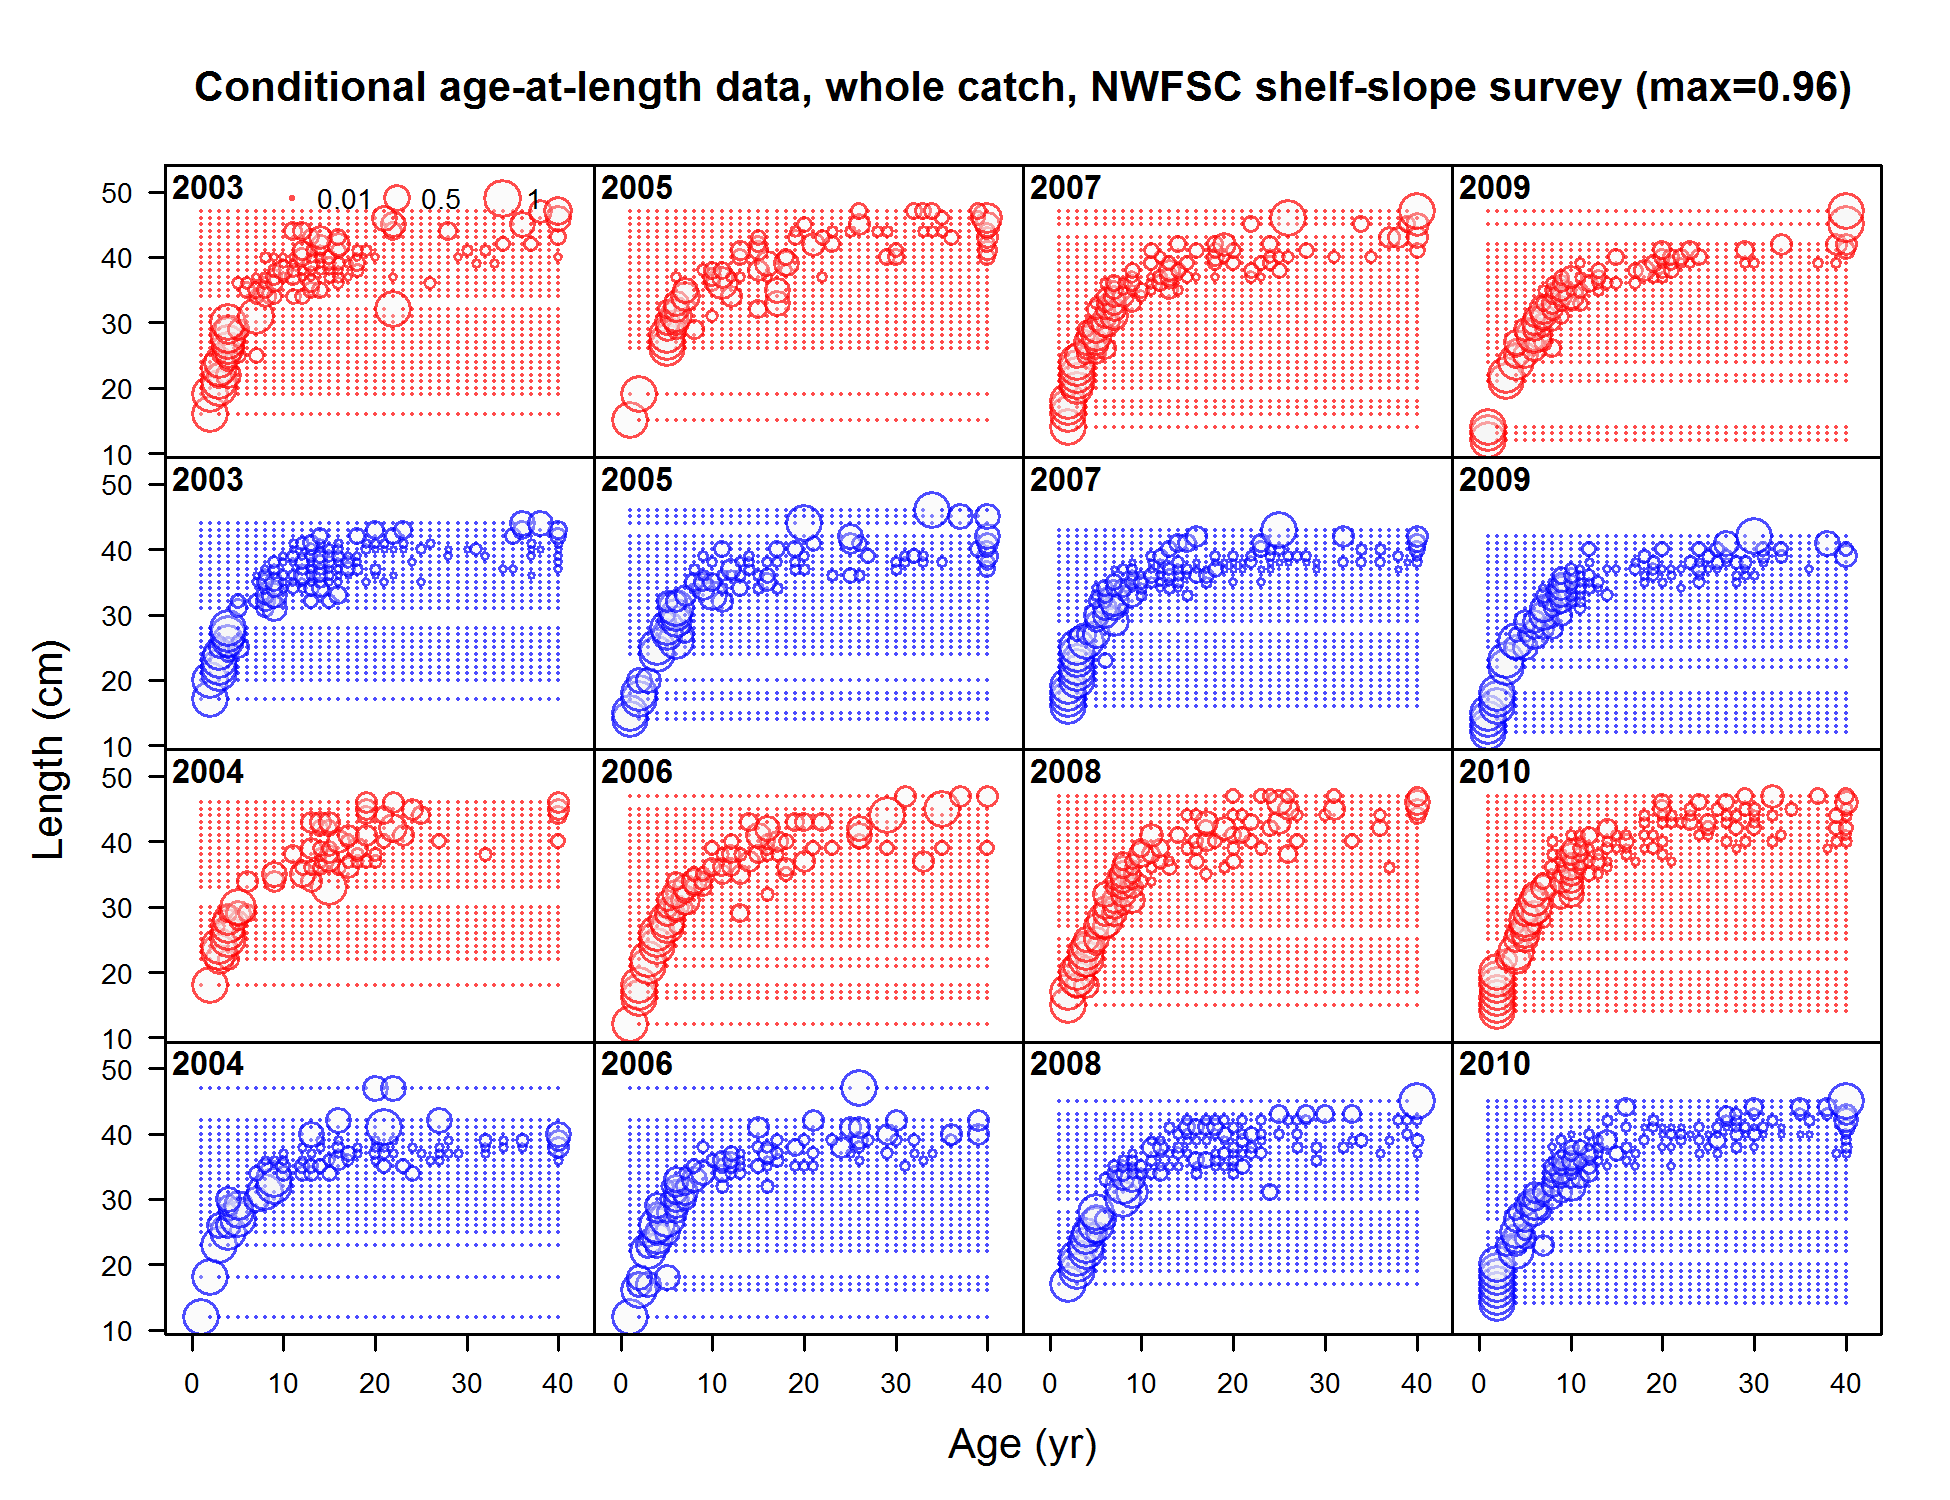
\includegraphics[scale = 0.37]{r4ss/comp_condAALdat_bubflt8mkt0_page1.png}
    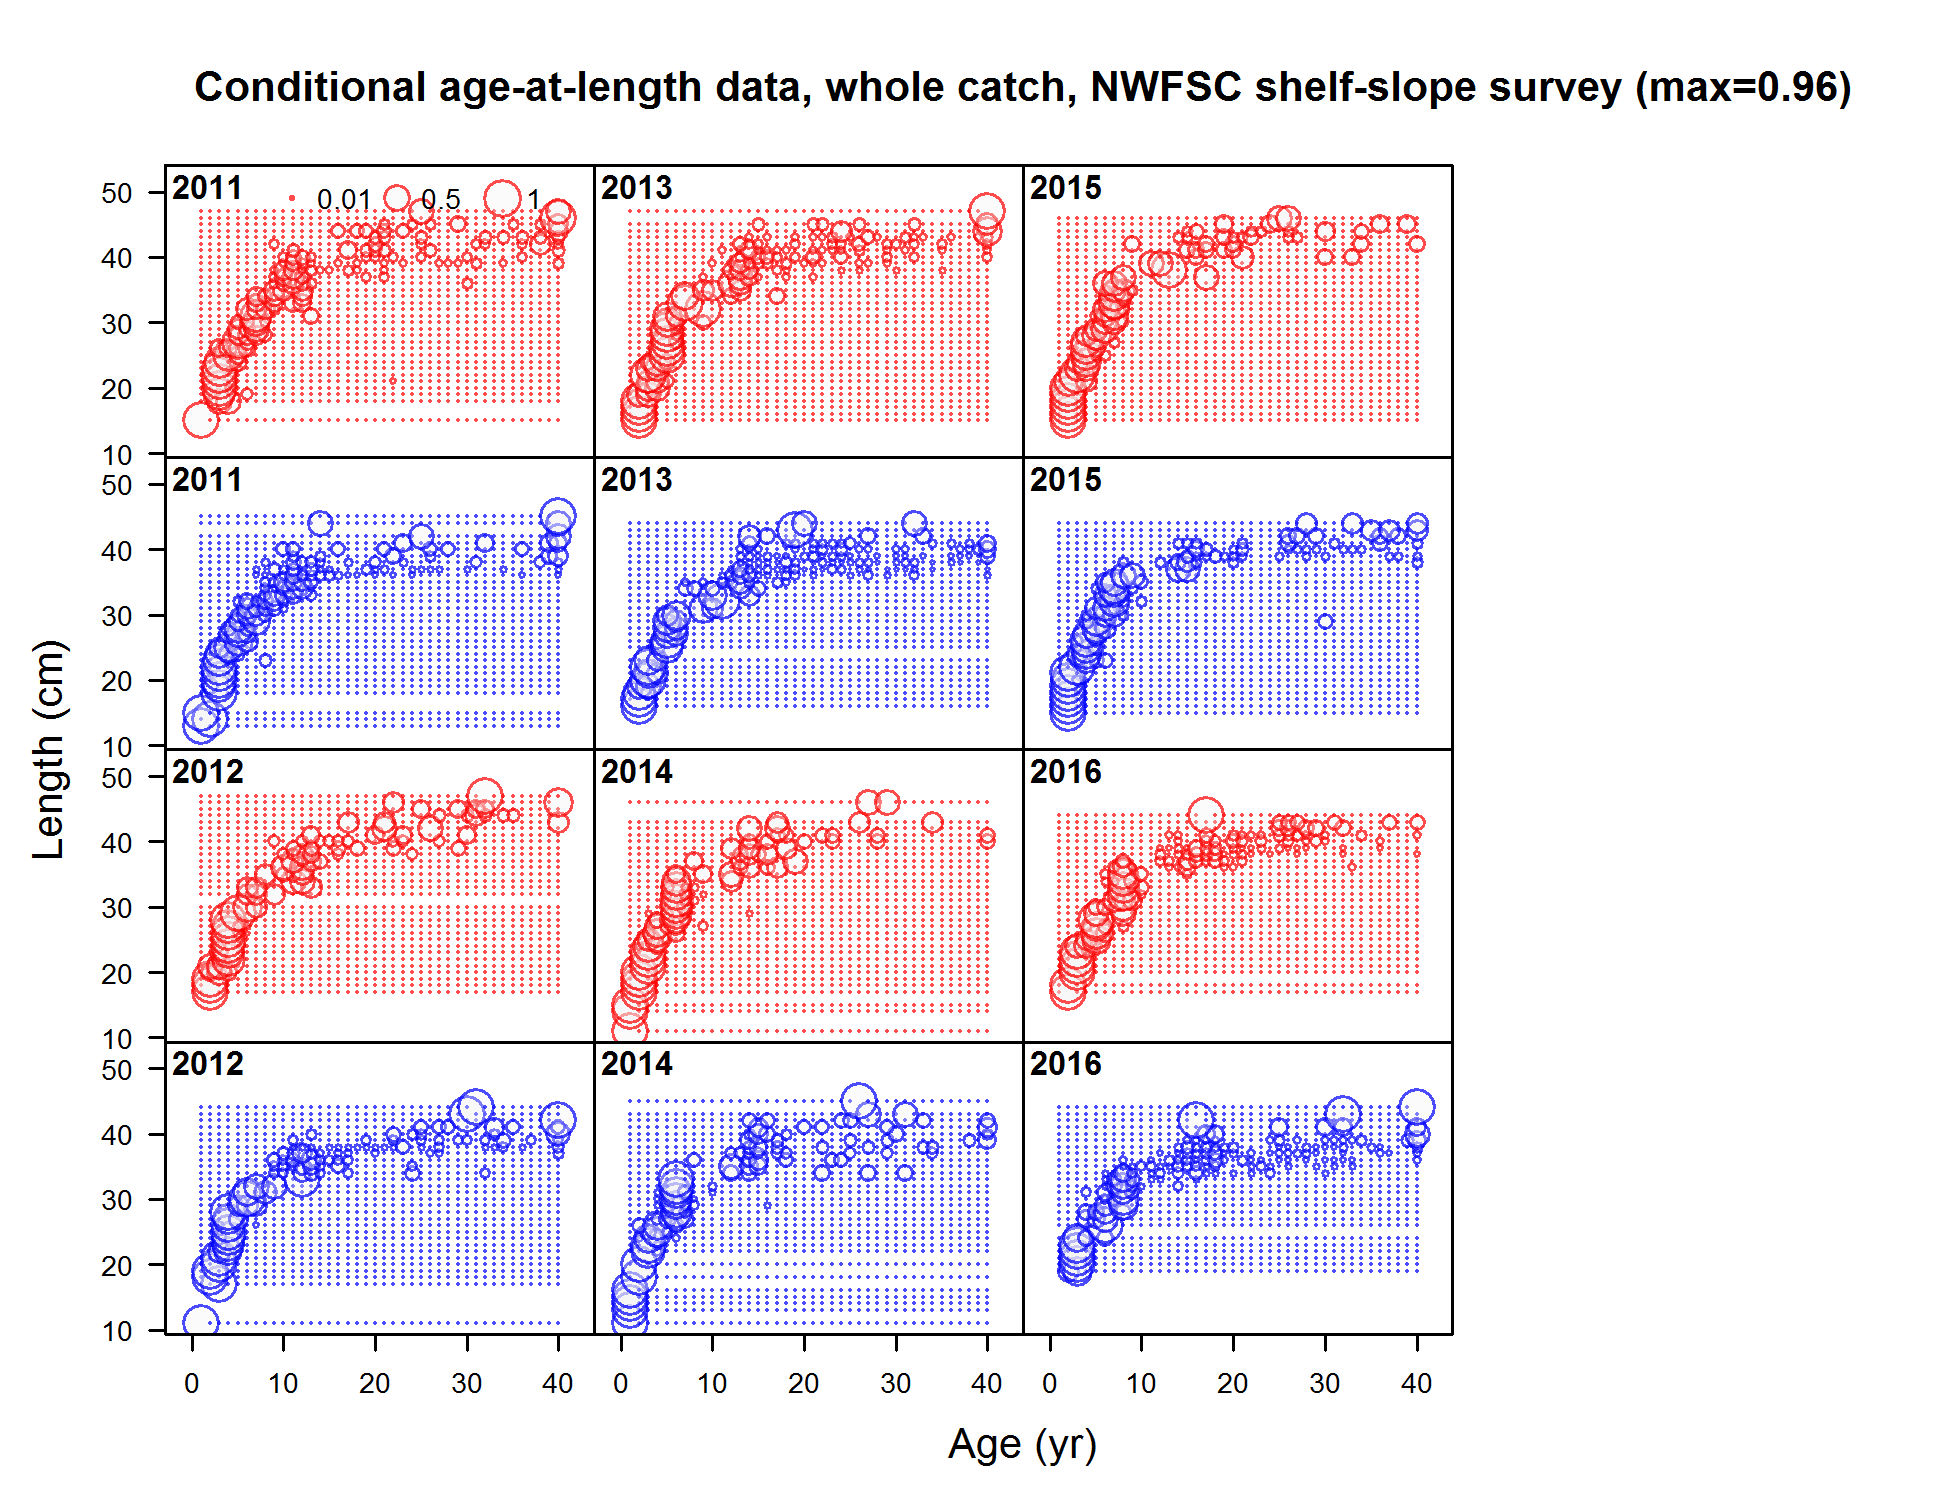
\includegraphics[scale = 0.37]{r4ss/comp_condAALdat_bubflt8mkt0_page2.png}
\end{frame}


\begin{frame}{Aggregated data by source}
    \includegraphics[scale = 0.37]{r4ss/comp_lendat__aggregated_across_time.png}
    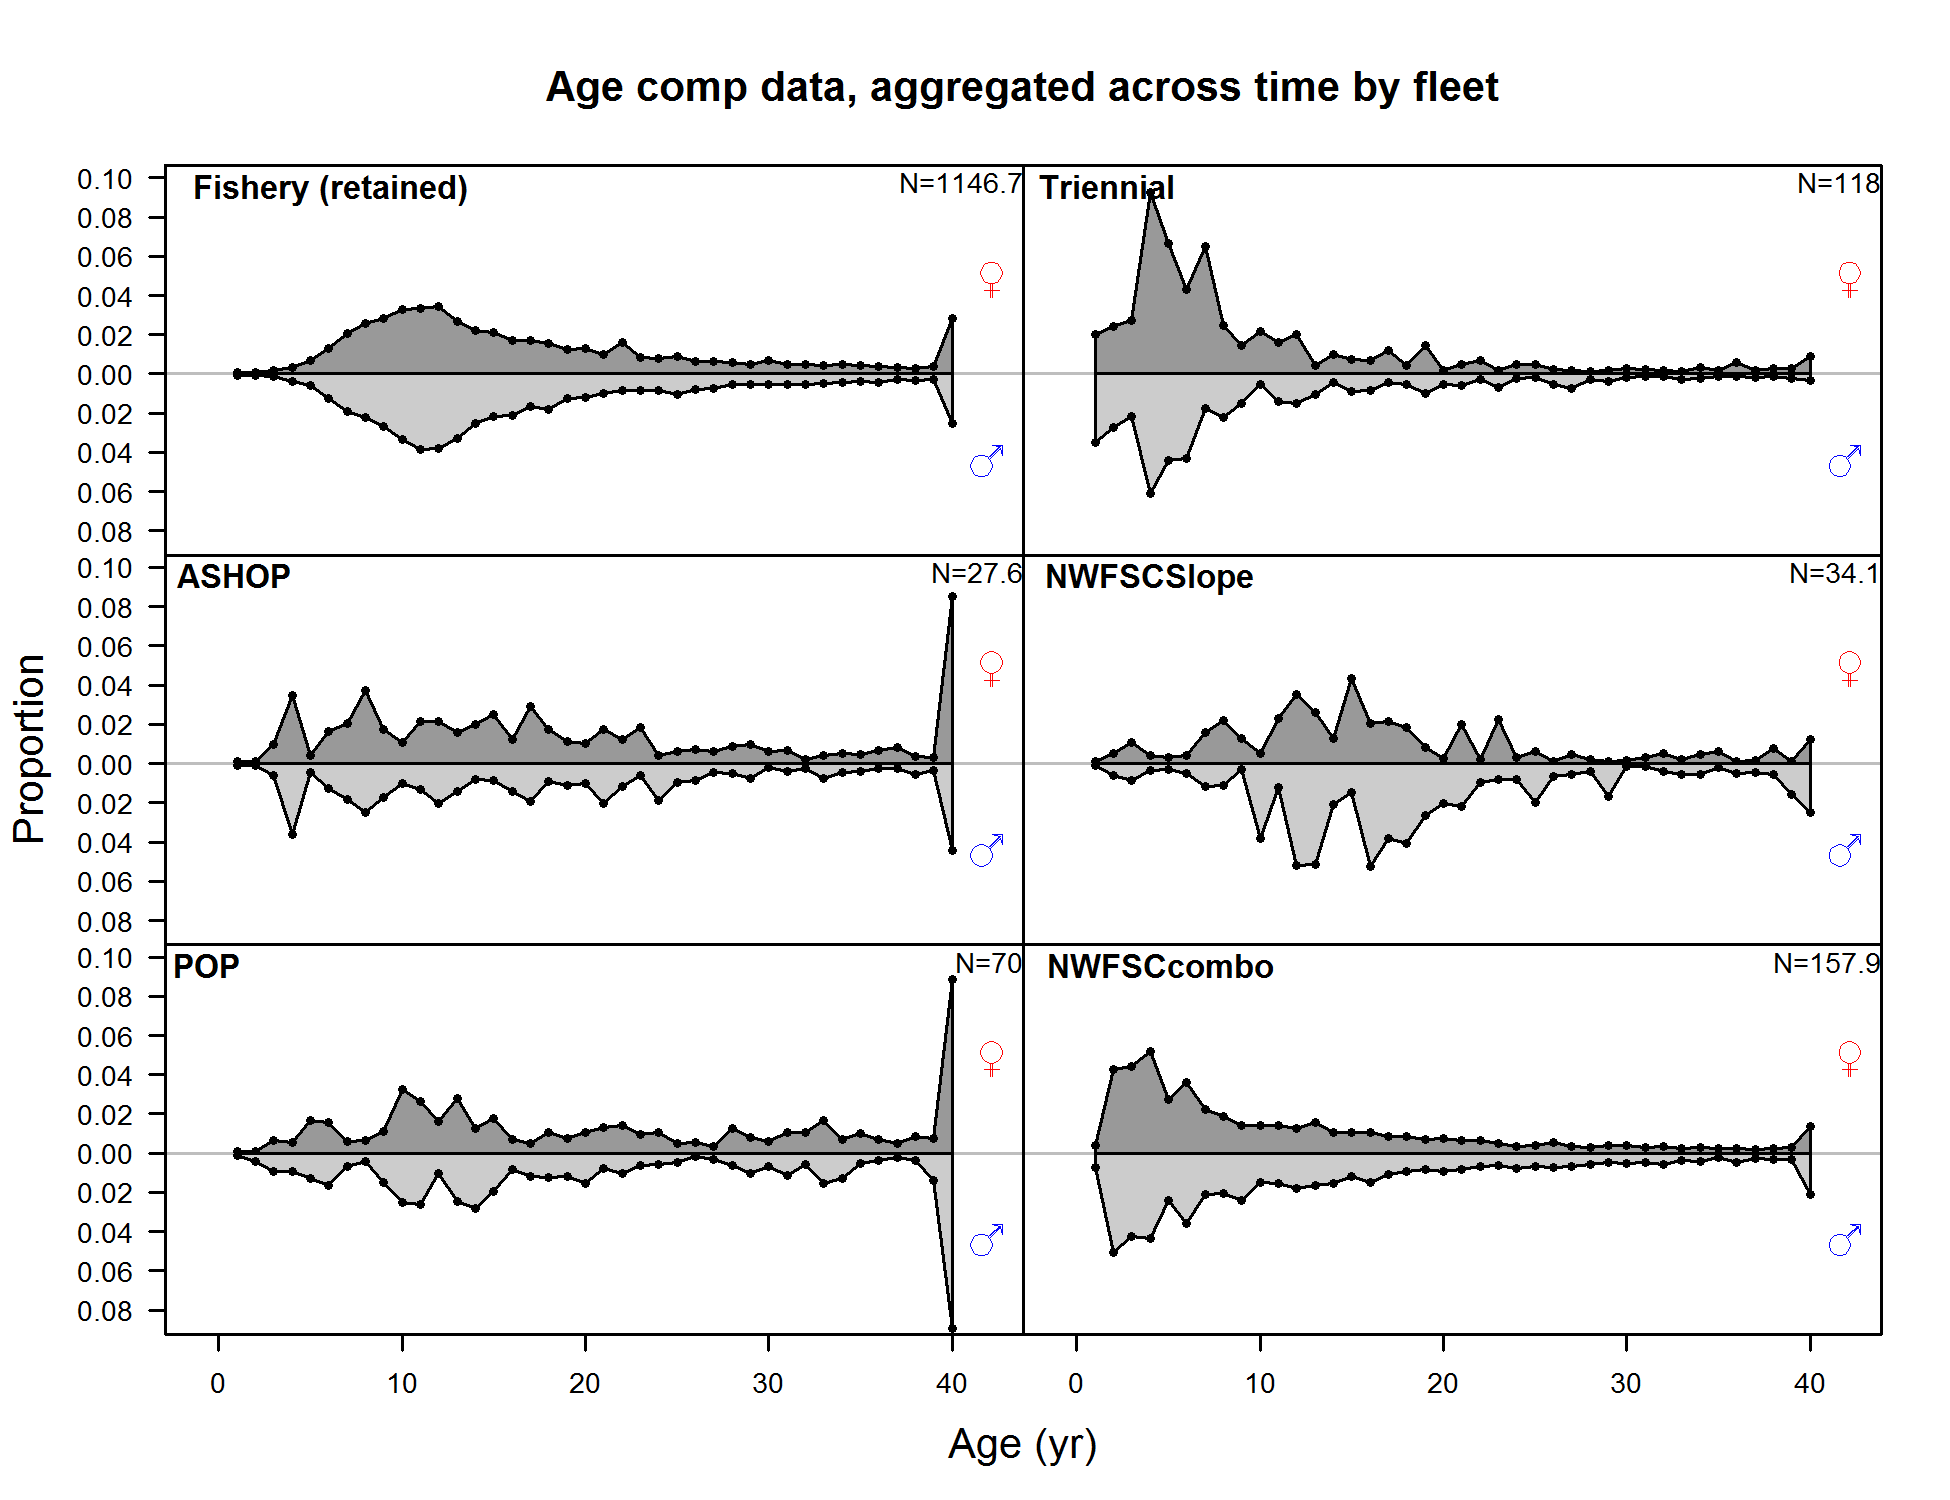
\includegraphics[scale = 0.37]{figures/comp_agedat__aggregated_across_time.png}
\end{frame}


\subsection{Ageing Error}
\begin{frame}{Estimated Ageing Error: Curvilinear without bias}
  \begin{center}
    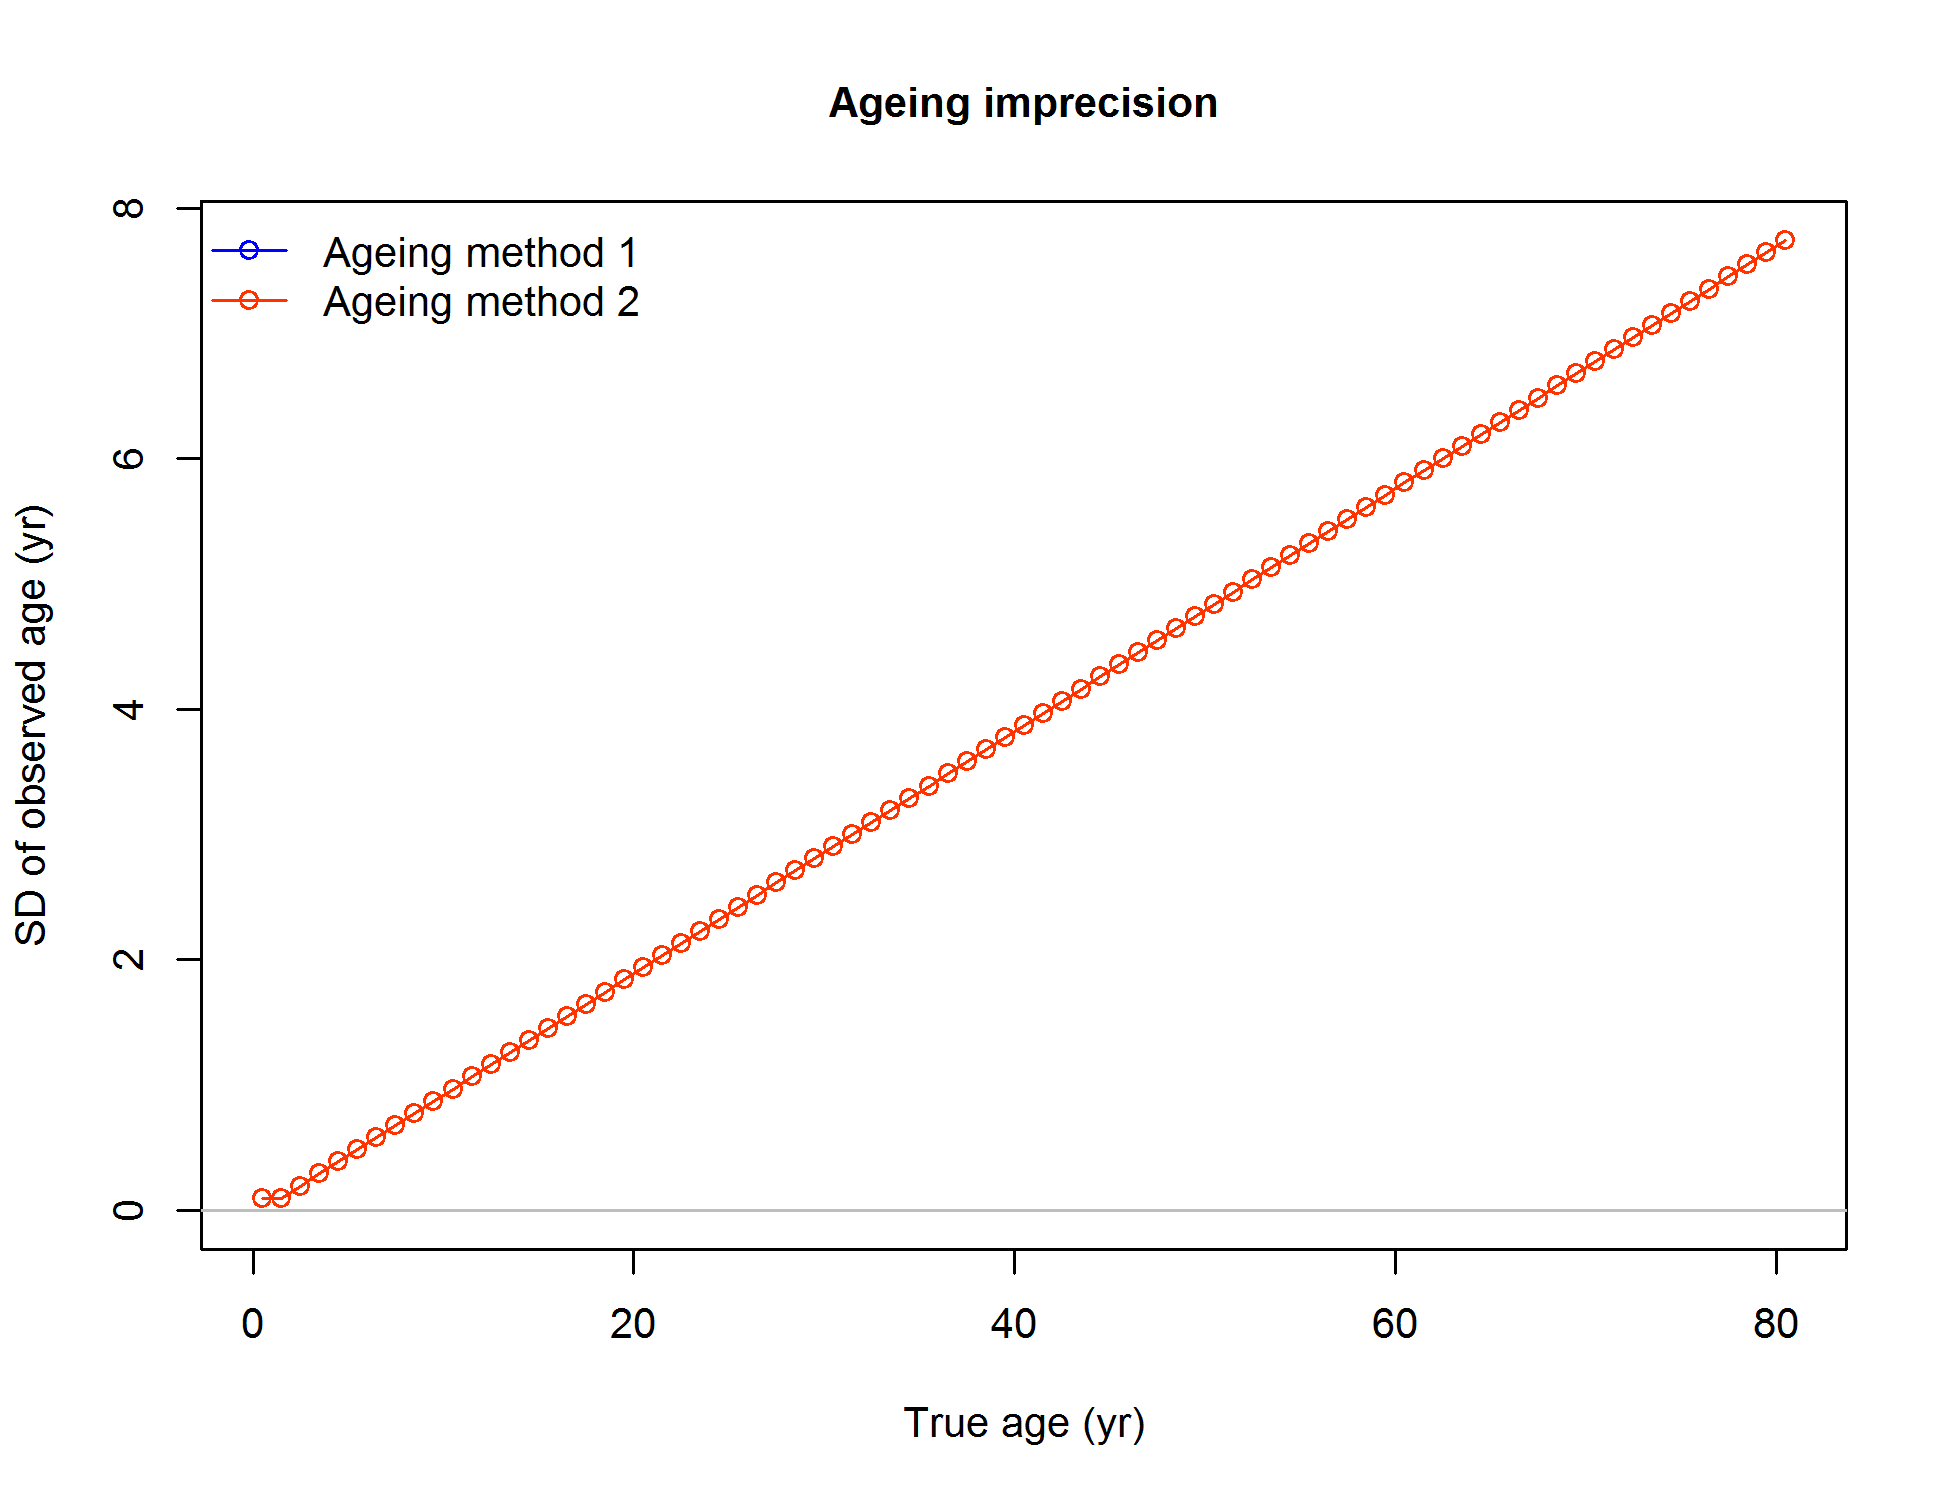
\includegraphics[scale = 0.50]{r4ss/numbers5_ageerrorSD.png}
  \end{center}
\end{frame}

\begin{frame}
  \Huge{\centerline{Conclusion of}}
  \Huge{\centerline{Biology \& Data}}
\end{frame}

%---------------------------------------------------------------------------
\section*{Appendix}
%-----------------------------------------------------------------------------
\begin{frame}{VAST vs. Bayesian Delta-GLMM Indices}
  \begin{center}
    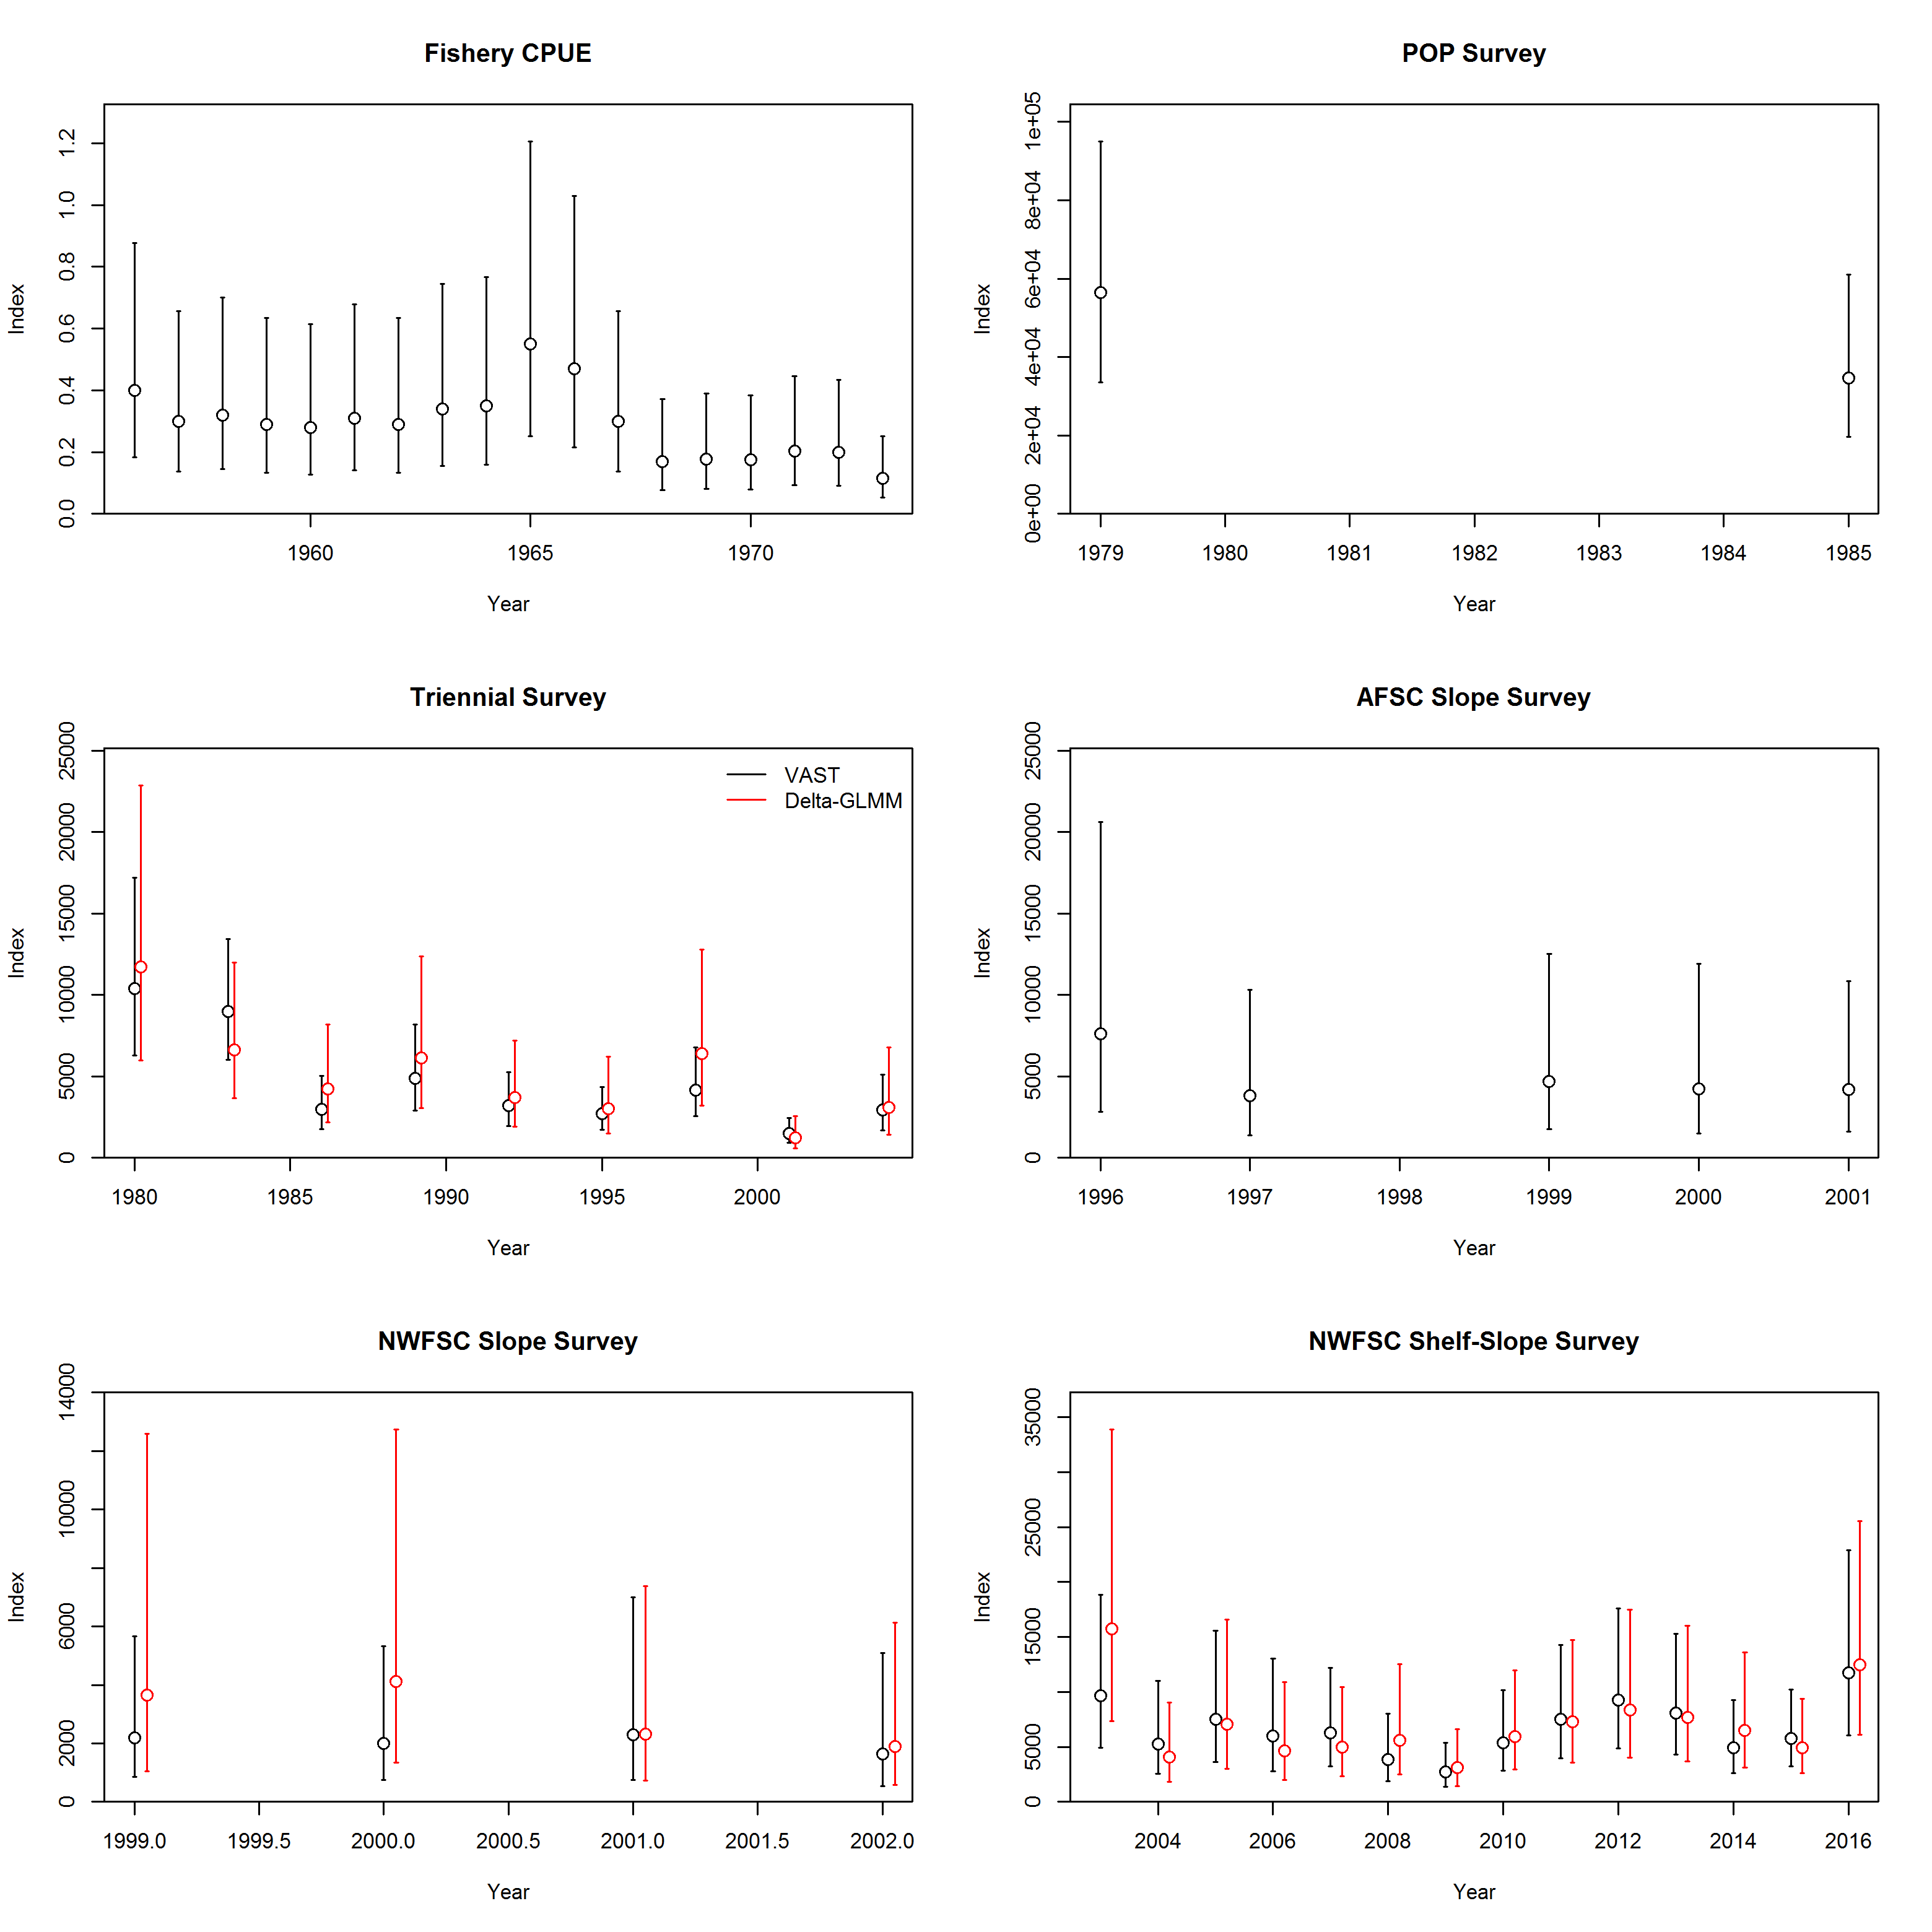
\includegraphics[scale = 0.30]{figures/Index_Comparison.png}
  \end{center}
\end{frame}  

\begin{frame}{Designed Based vs. VAST Indices}
  \begin{center}
    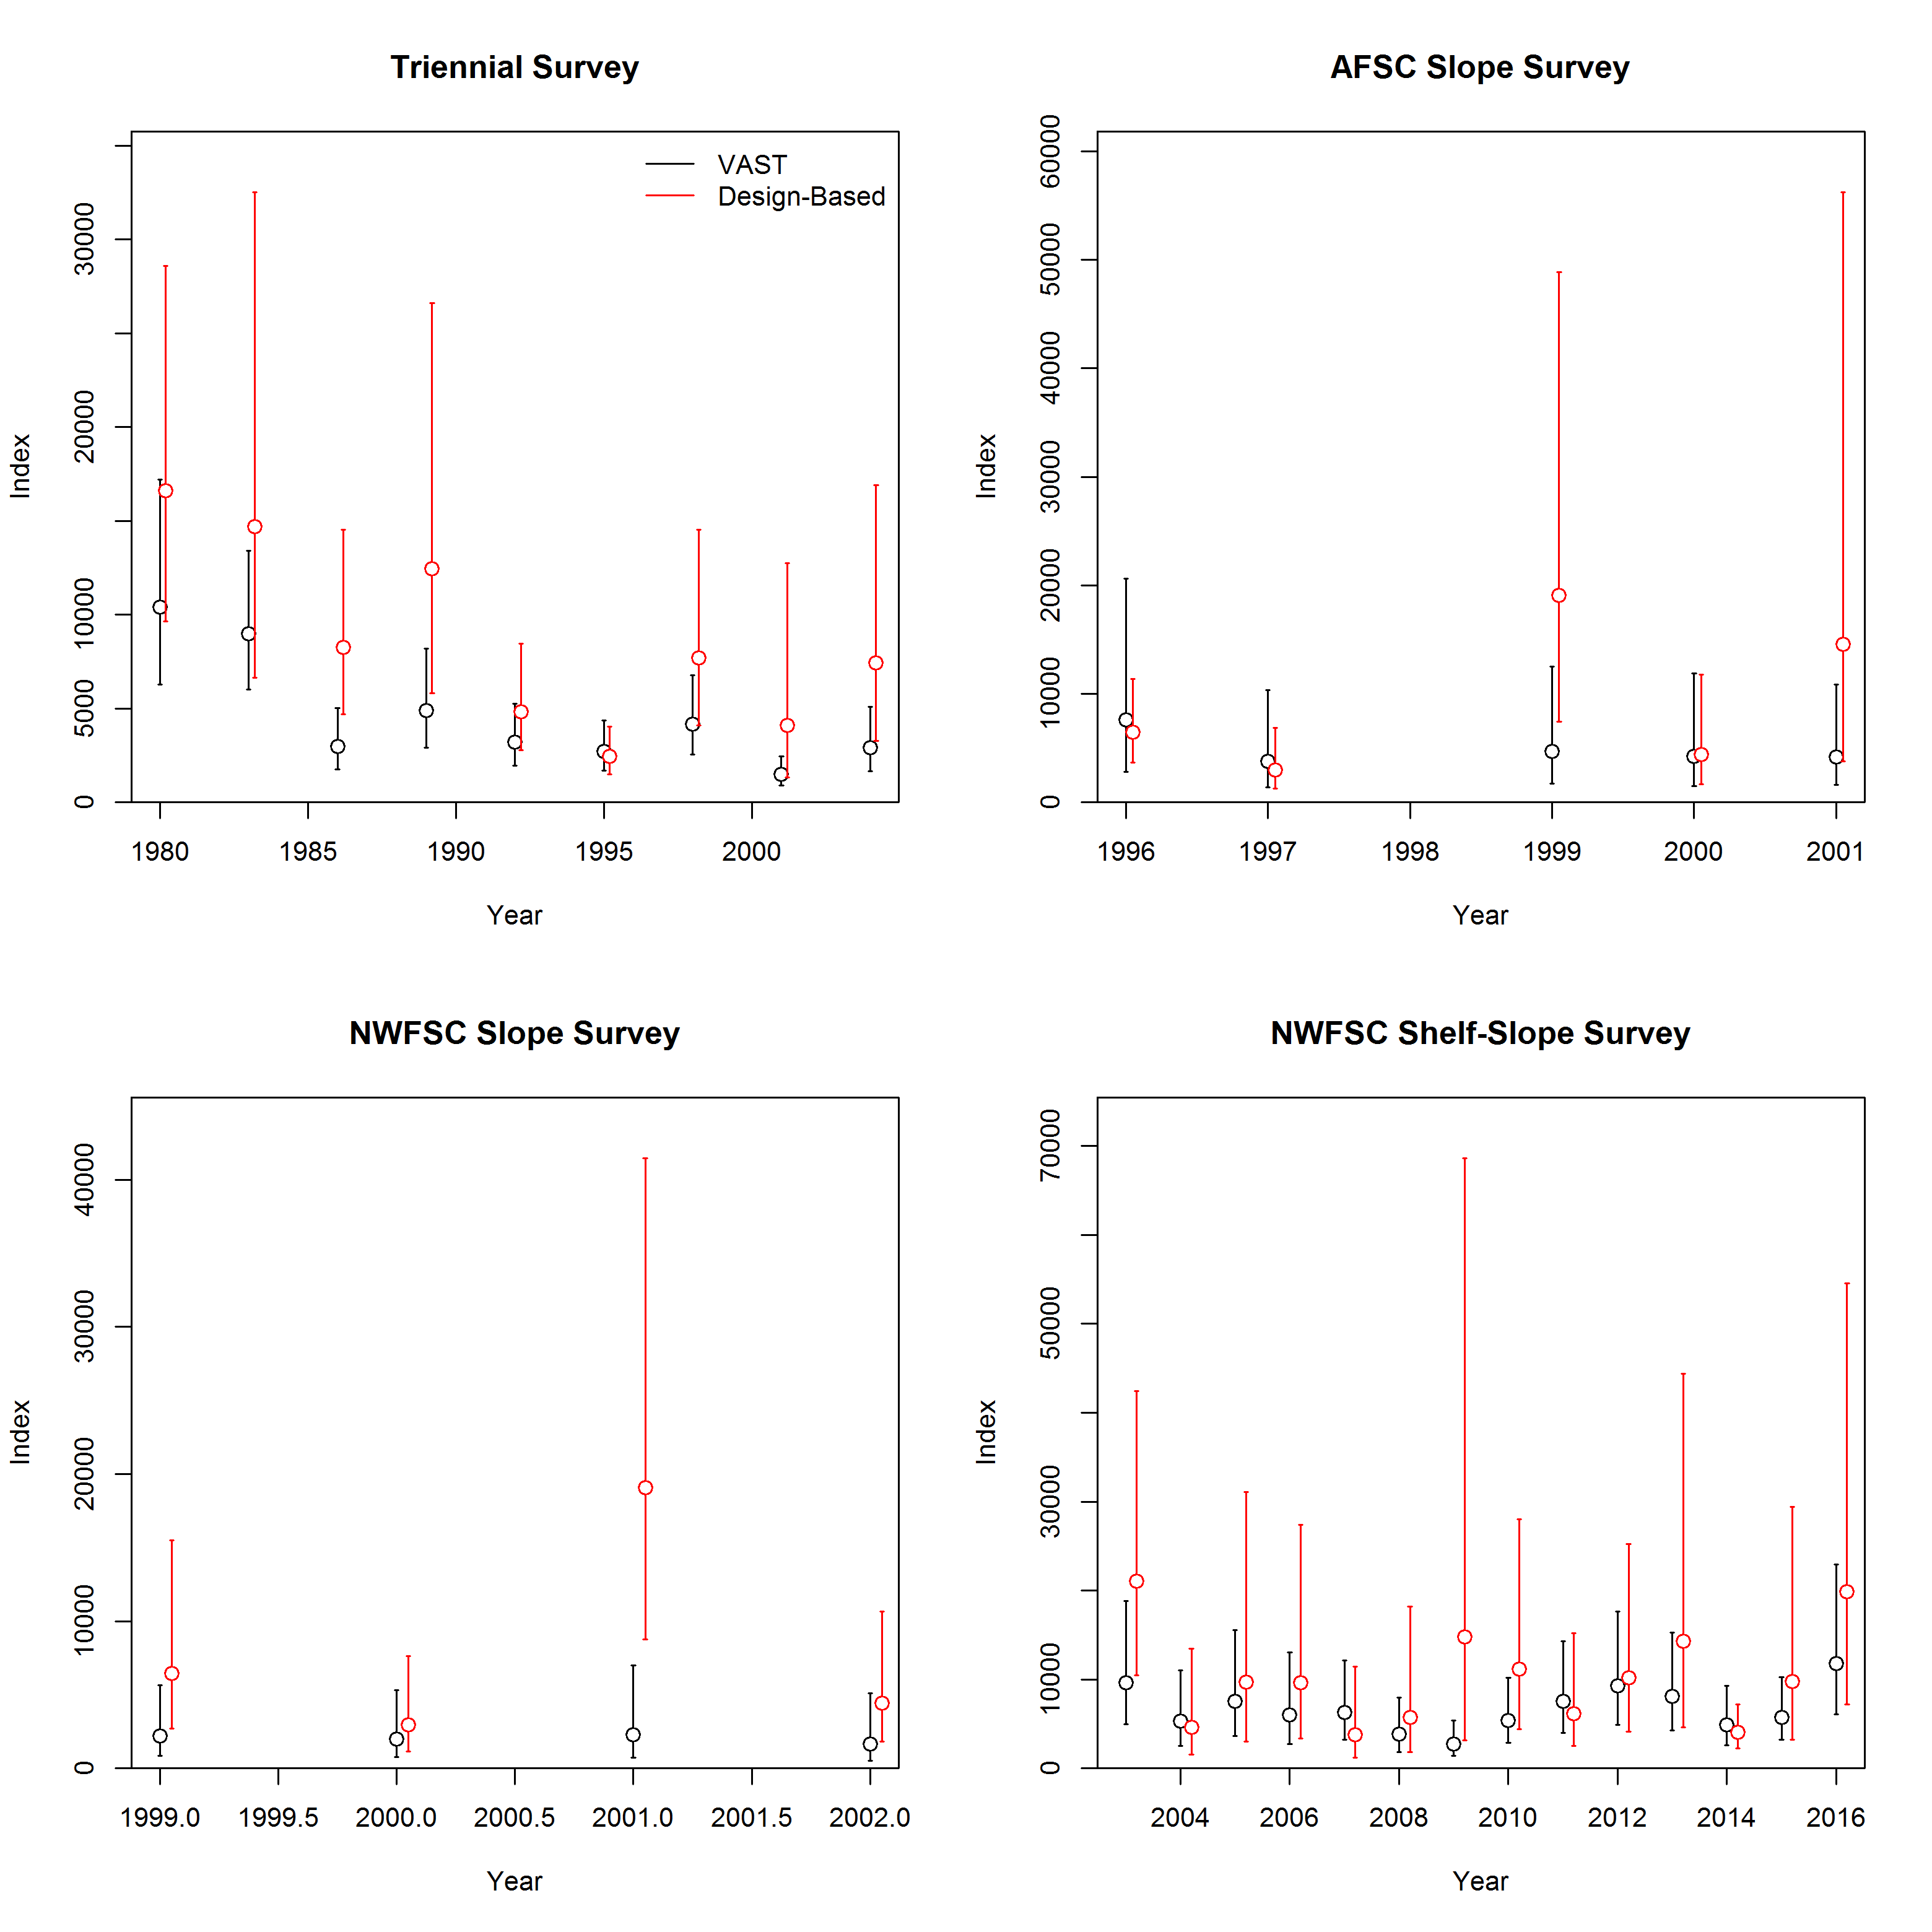
\includegraphics[scale = 0.30]{figures/Index_DesignBased_Comparison.png}
  \end{center}
\end{frame} 

\begin{frame}{Pre-Model 2011 Indices vs. 2017 Indices}
  \begin{center}
    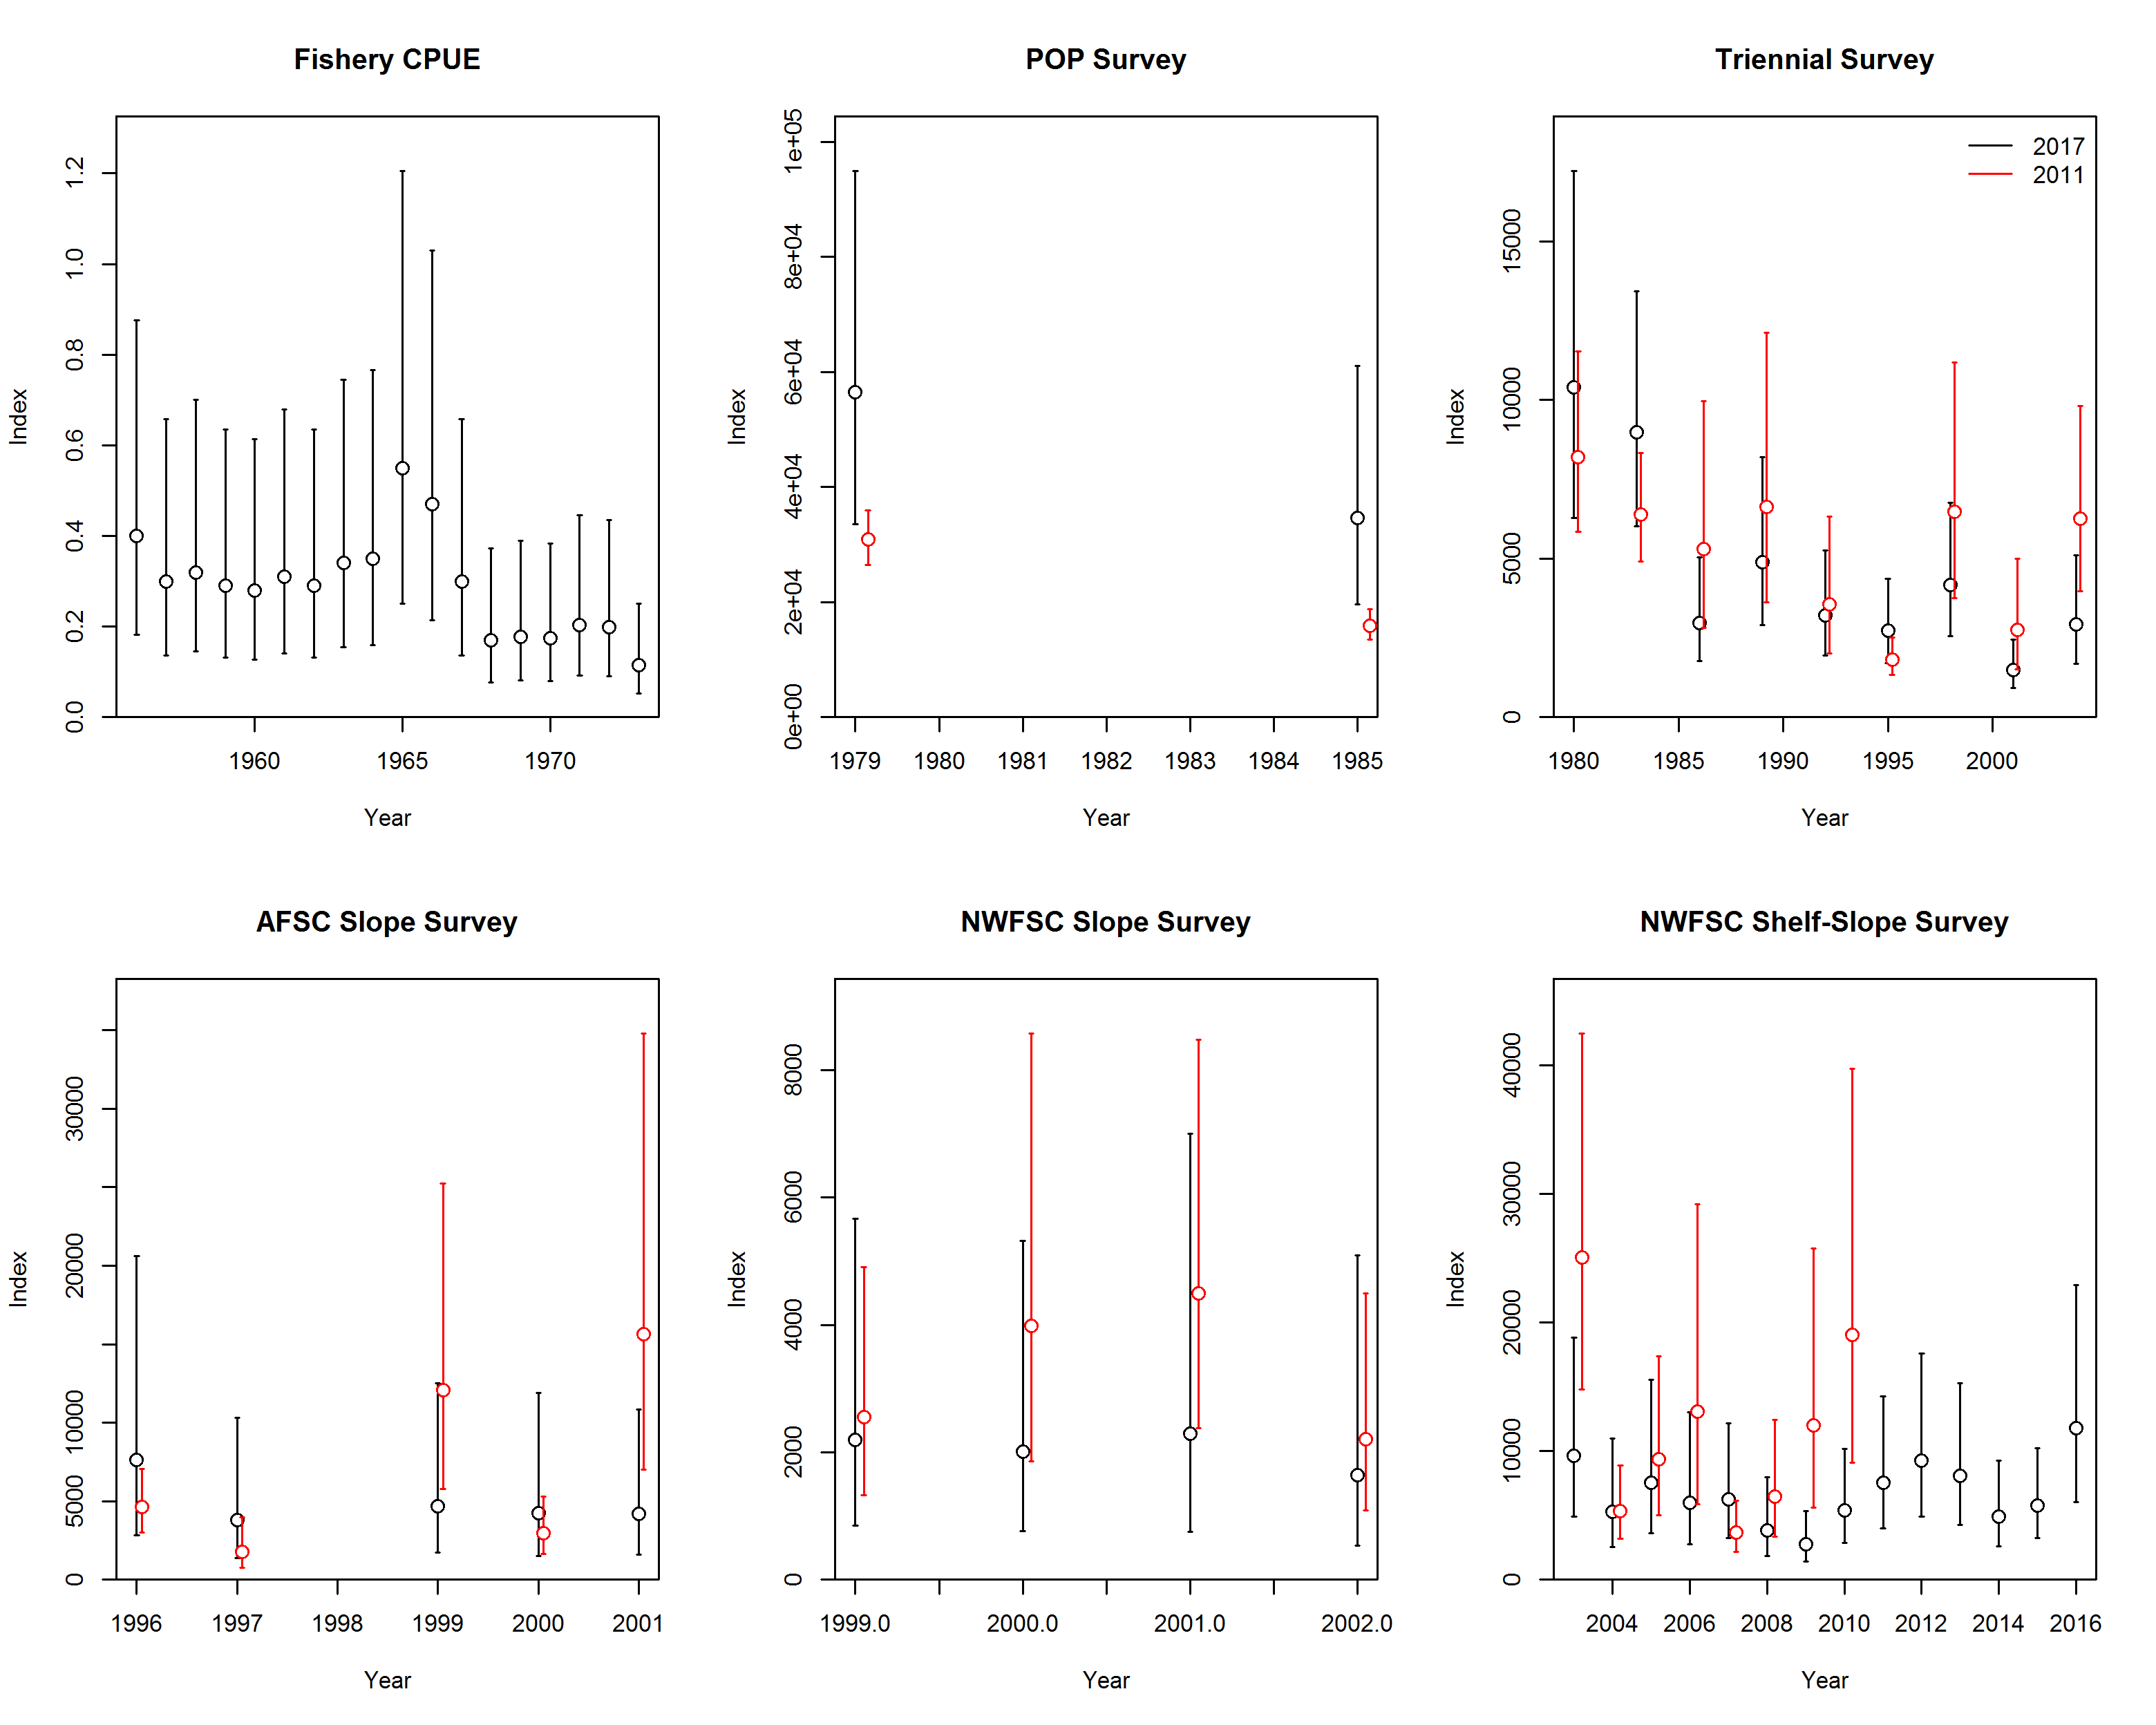
\includegraphics[scale = 0.35]{figures/Index_Compare_2011_2017.png}
  \end{center}
\end{frame} 

\begin{frame}{Post Model 2011 Indices vs. 2017 Indices}
  \begin{center}
    \includegraphics[scale = 0.35]{figures/Index_Compare_PostModel_2011_2017.png}
  \end{center}
\end{frame} 

\begin{frame}{Catchability Comparison}
  \begin{table}[ht]
  \centering
  \begin{tabular}{p{2in}p{0.7in}p{0.7in}}
  Index & 2011 & 2017 \\ 
  \hline
  Fishery CPUE & 5.25E-06 & 4.48E-06 \\ 
  Pacific ocean perch survey & 0.8126 & 0.8741 \\
  Triennial shelf survey (early)& 0.2423 & 0.161 \\ 
  Triennial shelf survey (late) & 0.1793 & - \\
  AFSC slope survey & 0.2708 & 0.0822 \\ 
  NWFSC slope survey & 0.1717 & 0.0571 \\
  NWFSC shelf-slope survey & 0.4797 & 0.0728 \\
  \hline
  \end{tabular}
  \end{table}
\end{frame}


\begin{frame}{2011 vs. 2017 NWFSC shelf-slope index}
  \begin{center}
    \includegraphics[scale = 0.20]{figures/NWFSC_shelf_slope_2011_2017.png}
  \end{center}
\end{frame} 
  
\end{document}
